%%%%%%%%%%%%%%%%%%%%%%%%%%% asme2ej.tex %%%%%%%%%%%%%%%%%%%%%%%%%%%%%%%
% Template for producing ASME-format journal articles using LaTeX    %
% Written by   Harry H. Cheng, Professor and Director                %
%              Integration Engineering Laboratory                    %
%              Department of Mechanical and Aerospace Engineering    %
%              University of California                              %
%              Davis, CA 95616                                       %
%              Tel: (530) 752-5020 (office)                          %
%                   (530) 752-1028 (lab)                             %
%              Fax: (530) 752-4158                                   %
%              Email: hhcheng@ucdavis.edu                            %
%              WWW:   http://iel.ucdavis.edu/people/cheng.html       %
%              May 7, 1994                                           %
% Modified: February 16, 2001 by Harry H. Cheng                      %
% Modified: January  01, 2003 by Geoffrey R. Shiflett                %
% Modified: July 19, 2009 as a template in a single column for       %
%           ASME Journals by Harry H. Cheng                          %
% Use at your own risk, send complaints to /dev/null                 %
%%%%%%%%%%%%%%%%%%%%%%%%%%%%%%%%%%%%%%%%%%%%%%%%%%%%%%%%%%%%%%%%%%%%%%

%%% use 10pt options with the asme2ej format
%\documentclass[10pt]{asme2ej}
\documentclass[11pt,cleanfoot]{asme2ej}

\usepackage{graphicx} %% for loading jpg figures
\usepackage{epsfig}
\usepackage{fancyhdr}
\usepackage{setspace}
\usepackage{helvet}
\usepackage{amsmath}
\usepackage{enumitem}
\usepackage[hyphens]{url}
%\usepackage{hyphens}
\renewcommand{\familydefault}{\sfdefault}
\pagestyle{fancy}
\lhead{{\it Journal of Vibration and Acoustics}}
\rhead{}
\renewcommand{\headrulewidth}{0pt}
\topmargin 80 pt
\headheight 14 pt
\headsep 30 pt
%\RequirePackage[hyphens]
\usepackage{hyperref}   % to set up hyperlinks
\hypersetup{
	colorlinks=true,
	linkcolor=blue,
	citecolor=blue,
	urlcolor=blue,
}
\usepackage[square,numbers]{natbib}

%% The class has several options
%  onecolumn/twocolumn - format for one or two columns per page
%  10pt/11pt/12pt - use 10, 11, or 12 point font
%  oneside/twoside - format for oneside/twosided printing
%  final/draft - format for final/draft copy
%  cleanfoot - take out copyright info in footer leave page number
%  cleanhead - take out the conference banner on the title page
%  titlepage/notitlepage - put in titlepage or leave out titlepage
%  
%% The default is oneside, onecolumn, 10pt, final

\usepackage{lineno}   % For line numbering
\usepackage{xcolor}

\title{Flow noise estimation models for axial flow past towed sonar arrays}

%%% first author
\author{Rakesh Sekharipuram Sekar
    \affiliation{
	Department of Mechanical Engineering,\\
Indian Institute of Technology Palakkad,\\
Palakkad, Kerala, 678003, India \\
Email: 132203001@smail.iitpkd.ac.in
    }	
}

%%% second author
%%% remove the following entry for single author papers
%%% add more entries for additional authors
\author{Senthil Rajan S \\
    \affiliation{ Naval Physical Oceanographic Laboratory, \\
Ernakulam, Kerala, 682021, India\\
        Email: senthilrajan.npol@gov.in
    }
}

%%% third author
%%% remove the following entry for single author papers
%%% add more entries for additional authors
\author{Anoop Akkoorath Mana\thanks{Address all correspondence for other issues to this author.}\\
	\affiliation{Department of Mechanical Engineering,\\
Indian Institute of Technology Palakkad,\\
Palakkad, Kerala, 678003, India\\
Email: akkoorath@iitpkd.ac.in
    }
}


\begin{document}

\maketitle    
\doublespacing
\linenumbers
\renewcommand{\linenumberfont}{\normalfont\bfseries\color{red}}
%%%%%%%%%%%%%%%%%%%%%%%%%%%%%%%%%%%%%%%%%%%%%%%%%%%%%%%%%%%%%%%%%%%%%%
\begin{abstract}
{\it 
Towed sonar arrays house a series of pressure sensors inside a fluid-filled elastic tube. Towing of the sonar array in water generates a turbulent boundary layer on the exterior surface of the elastic tube. The pressure fluctuations in the turbulent boundary layer along with other ambient pressure fluctuations, excites the elastic tube and further generates pressure disturbances in the interior fluid. In this work, a new semi-empirical model of the turbulent pressure spectrum is presented. The new model predictions show a closer agreement with the available experimental results at all tow speeds. A three-dimensional vibroacoustic model of the fluid-filled elastic tube is also presented in this work. The vibroacoustic model is fully coupled and considers both breathing mode and first order variations in the elastic tube and the acoustic field variables. Further, the turbulent pressure spectrum semi-empirical model and the three-dimensional vibroacoustic model are used to compute the on-axis sound pressure level due to the external turbulent pressure excitation at different elastic tube diameters and tow speeds. At low frequencies, increasing tube diameter has little effect on flow noise, while at higher frequencies, flow noise decreases with larger diameters. Increasing tow speed raises flow noise across all frequencies.
}
\end{abstract}

%%%%%%%%%%%%%%%%%%%%%%%%%%%%%%%%%%%%%%%%%%%%%%%%%%%%%%%%%%%%%%%%%%%%%%
%\begin{nomenclature}
%\entry{A}{You may include nomenclature here.}
%\entry{$\alpha$}{There are two arguments for each entry of the nomemclature %environment, the symbol and the definition.}
%\end{nomenclature}

%The primary text heading is  boldface and flushed left with the left margin.  %The spacing between the  text and the heading is two line spaces.

%%%%%%%%%%%%%%%%%%%%%%%%%%%%%%%%%%%%%%%%%%%%%%%%%%%%%%%%%%%%%%%%%%%%%%

\section*{Introduction}

Towed sonar arrays contain a series of pressure sensors enclosed within a fluid-filled elastic tube. As the sonar array is towed through the water, a thick layer of turbulent flow is generated over the exterior surface of the tube.~The pressure fluctuations in this turbulent boundary layer (TBL), along with other ambient sea pressure variations, excite the elastic tube and subsequently produce acoustic pressure disturbances within the interior fluid. The hydrophones placed in the interior fluid picks these acoustic signals. The signals associated with the turbulent pressure fluctuations are called flow noise. Currently, the flow noise is measured either by towing the sonar array in open water using a dinghy or by allowing the hydrophone to free fall in water \cite{Sarath2010}. In the first case, noise from the boat and vibrations of the towline connections pollute the measured acoustic signals \cite{Unni2011}; whereas in the second case, the useful measurements can be made only at the terminal velocity of the hydrophone. This work aims at developing a fully-coupled vibroacoustic model for predicting the flow noise in towed sonar arrays which is useful over wide range of towing speeds and tube diameters.

%\subsection{Flow over a flat plate}
A widely used model for predicting the turbulent pressure spectrum is that developed by Corcos \cite{corcos1963} for the flow over a flat plate. In this model, the turbulent pressure is varying exponentially with respect to both the axes of the flat plate. Although this model is widely used in engineering applications, it has a major shortcoming that it is overestimating the pressure level at low wavenumbers. Chase \cite{Chase1981} presented a simpler turbulent pressure spectrum model for the flow over a flat plate. The model is based on experimental observations and uses direct dependence on the flow and dimensional parameters. Frendi and Zhang~\cite{frendi2020} analysed the Corcos \cite{corcos1963} model and proposed a turbulent model for the flow over a flat plate based on large eddy simulation (LES) and direct numerical simulation (DNS) computational results. Frendi's model involves the use of an auto spectrum which was derived by Goody \cite{goody2004}. The Frendi model predictions are found to match well with an earlier experimental result on flow over a flat plate. Some of the observations of the Chase and Frendi models are relevant to the present work and are discussed in section \ref{sec:empmodels}. Francis \textit{et al}.~\cite{francis2023} used LES and Reynolds averaged Navier Stokes (RANS) computational method to study the wavenumber frequency spectrum of the turbulent pressure field over a flat plate. This work presents an exhaustive discussion on similar problems in the literature.

%\subsection{Axial flow past a cylinder}
Chase~\cite{Chase1981} developed a model for computing the turbulent pressure spectrum for an axial flow past a cylinder by modifying his earlier flat plate model. While modifying, Chase considered the radius of the cylinder as one of the parameters instead of the length of the flat plate. Chase derived azimuthal harmonic spectral density by integrating the turbulent pressure spectrum of the flat plate in the cross-flow direction. The details of this model are presented in section \ref{Chase model}. 


Carpenter and Kewley~\cite{carpenter1983} conducted experiments for finding the flow noise inside a fluid-filled elastic tube while towed behind a ship and compared the results with that predicted by  Chase~\cite{Chase1981}. The authors also proposed a tube transfer function for computing the flow noise inside the tube. Knight~\cite{knight1996} performed similar analytical simulations as in \cite{carpenter1983} but with different types of hydrophones and compared the flow noise with that for an ideal hydrophone. The ideal hydrophone was assumed to have unit acoustic response and zero convective response. Knight also used an approximate tube transfer function to find the noise inside the fluid-filled elastic tube.\par


Unnikrishnan \textit{et al}.~\cite{Unni2011} performed experiments to measure the turbulent pressure field outside the elastic tube by towing the sonar array in a quiet lake at different speeds. The work presents a comparison of the experimental results with the available semi-empirical model predictions. It was found that the semi-empirical model estimations match with the measurements only at high tow speeds. Karthik \textit{et al}.~\cite{karthik2021} studied the turbulent pressure spectrum over a cylinder with the help of an LES computational model. The model predictions match well with the experimental results of Unnikrishnan \textit{et al}.~\cite{Unni2011}. Karthik \textit{et al}. also presented a non-dimensional turbulent flow noise spectrum for easy estimation of the spectrum at different tow speeds and tube diameters.

Both Carpenter and Kewley~\cite{carpenter1983} and Knight~\cite{knight1996} estimated the flow noise inside a fluid-filled elastic tube with the help of the Chase model for the turbulent pressure spectrum and an approximate tube transfer function. Jineesh and Ebenezer~\cite{jineesh2013} developed a better axisymmetric model of the fluid-filled elastic tube and used it to estimate the flow noise inside the tube. It was found that the earlier approximate transfer function model overestimated the flow noise inside the tube.

This paper develops a new semi-empirical model of the turbulent pressure spectrum for axial flow past a solid cylinder. It also presents a fully coupled three-dimensional vibroacoustic model of a fluid-filled elastic tube. Furthermore, these two models are used to compute the on-axis sound pressure level resulting from an external turbulent pressure excitation on the elastic tube. This paper is organized as follows: Section~\ref{sec:empmodels} discusses two existing semi-empirical models for estimating turbulent pressure spectrum for axial flow past a solid cylinder. Section~\ref{sec:hybmodel} discusses the development of a new semi-empirical model for the turbulent pressure spectrum, which provides improved predictions compared to existing models. Section~\ref{sec:vamodel} discusses the development of a three-dimensional vibroacoustic model for estimating the on-axis flow noise inside a fluid-filled elastic tube. Further, Section~\ref{sec:results} presents the results on interior acoustic pressure spectrum and on-axis flow noise inside a fluid-filled elastic tube and are compared with the available results in the literature.
%%%%%%%%%%%%%%%%%%%%%%%%%%%%%%%%%%%%%%%%%%%%%%%%%%%%%%%%%%%%%%%%%%%%%%
\section{Review of semi-empirical models of turbulent pressure spectrum} \label{sec:empmodels}

One of the objective of this study is to predict the flow noise resulting from turbulent boundary layer excitation. To achieve this, a semi-empirical model that can estimate the turbulent pressure exerted by fluid flow on a cylindrical tube, is required. Two existing semi-empirical models for turbulent pressure fluctuation are discussed in this section. Further, flow noise at the outer surface of the tube is estimated using these models, showing its variation in comparison to available experimental results~\cite{Unni2011}. 
%\label{pressure spectrum}
%%%%%%%%%%%%%%%%%%%%%%%%%%%%%%%%%%%%%%%%%%%%%%%%%%%%%%%%%%%%%%%%%%%%%%%%%%%%%%%
\subsection{Chase model}\label{Chase model}
Chase~\cite{Chase1981} proposed a semi-empirical model for predicting the frequency-wavenumber spectrum of turbulent pressure field over a solid cylinder and is given by
\begin{equation}\label{Turbulent pressure spectrum equation Chase}
        \Hat{p}_{0}(k_{z},\omega) = C\rho^{2}\nu_{*}^{3}R^2\biggl[(k_{z}R)^{2}+\frac{1}{12}\biggr]\times \biggl[\frac{(\omega R-u_{c}k_{z}R)^{2}}{h^{2}\nu_{*}^{2}}+(k_{z}R)^{2}+b_1^{-2}\biggr]^{-2.5}.
\end{equation}
The important parameters in the above equation are axial wavenumber $k_{z}$, frequency $\omega$, density of the fluid $\rho$, convective speed $u_{c}$ ($=0.68u$, where $u$ is the tow speed), $C=0.063$, $h=3.7$, $\nu_{*}=0.04U$ and tube radius $R$~\cite{Chase1981, carpenter1983, knight1996, KUTTANCHANDRIKA2014, Huang2020}.
%% Use \subsection commands to start a subsection.
\subsection{Frendi model}
\label{Frendi model}
Frendi's model for the turbulent pressure spectrum for a flat plate is given by \cite{frendi2020}
\begin{equation}\label{Pressure spectrum equation from Frendi}
    \Hat{R}(k_{z},k_{2},\omega) = C_{1}R^{*}(\omega)e^{-\Hat{\alpha}r_{k}}.
\end{equation}
In the above equation, $C_{1}$ is given by
\begin{equation}\label{C1 equation}
C_{1} = \alpha^{2}m\delta^{2}\frac{1}{2\pi},   
\end{equation}
where $\alpha$ can be computed using
\begin{equation}\label{alpha equation}
   \alpha = \frac{a_1}{\pi}\frac{1}{\sqrt{1+a_2(\frac{\omega \delta}{u_{t}}-50)^{2}}}.
\end{equation}
In the above equation, $a_1=4.7$, $a_2=3\times10^{-5}$~\cite{frendi2020}, $u_{t}$ is the friction velocity (=0.04$u$, a small fraction of tow velocity $u$) and $\delta$ is the boundary layer thickness~\cite{Jordan2014} given by
\begin{equation}\label{boundary layer thickness}
    \delta = [48Re_a^{-1}Re_x^{(0.0226\log{Re_a}+0.2478)}]^{\frac{1}{0.91}}.
\end{equation}
In the above equation, $Re_a$ is the radius based Reynold's number ($\frac{\rho u R}{\mu}$) and $Re_x$ is length based Reynold's number ($\frac{\rho u x}{\mu}$), $x$ is distance of a point on the cylinder from the leading edge and $\mu$ is the dynamic viscosity of the fluid medium. The constant $m$ in Eq.~(\ref{C1 equation}) is a scaling factor which is approximately taken as 1/7.7~\cite{frendi2020}. 

$R^{*}(\omega)$ in Eq.~(\ref{Pressure spectrum equation from Frendi}) is the auto-spectrum given by~\cite{goody2004}
\begin{equation}\label{Auto spectrum equation from Goody}
    R^{*}(\omega) = \frac{3\tau_{w}^{2}\omega^{2}(\frac{\delta}{u})^{3}}{[(\frac{\omega \delta}{u})^{0.75} + 0.5]^{3.7} + [1.1R_{t}^{-0.57}(\frac{\omega \delta}{u})]^{7}}.
\end{equation}
In the above equation, $\tau_{w}$ is the shear stress at the wall, $R_{t}$ is the ratio of time scale~\cite{goody2004} given by
\begin{equation}\label{Time scale equation from Goody}
    R_{t} = \left (\frac{u_{t}}{u}\right)\left(\frac{u_{t}\delta}{\nu}\right),
\end{equation}
where $\nu$ is the kinematic viscosity. 

$\Hat{\alpha}$ in Eq.~(\ref{Pressure spectrum equation from Frendi}) is given by $\Hat{\alpha} = \alpha\delta$ and $r_{k}$ depends on the axial and crossflow wavenumbers and is given by 
\begin{equation}\label{rk equation}
    |{r_{k}}|^{2} = \bigg(k_{z} - \frac{\omega}{u_{c}}\bigg)^{2} + (mk_{2})^{2}.
\end{equation}
In the above equation, $k_{2}$ denotes the cross flow wavenumber and $u_{c}$ is the convective speed (= 0.68$u$, a large fraction of tow speed $u$). Eq.~(\ref{Pressure spectrum equation from Frendi}) can be modified for estimating turbulent pressure spectrum for an axial flow past a solid cylinder as
\begin{equation}\label{One D equation Frendi}
    \Hat{p}_0(k_{z},\omega) = \int_{-1/2R}^{1/2R}\Hat{R}(k_{z},k_{2},\omega)dk_{2}.
\end{equation}
% Brief how you're going to use the above models in this paper. Also, give a connect to the next section.
The estimation of flow noise using the models discussed in this section and its comparison with the findings of experiments are presented below.

\subsection{Flow noise} \label{sec:flownoise}
Here, the estimation of flow noise, as measured by a series of hydrophones placed at the outer surface of a solid cylinder, is discussed and compared with the experimental results~\cite{Unni2011}.
The flow noise associated with the turbulent pressure spectrum $p_{0}(k_{z},\omega)$ as registered by an array of hydrophones is~\cite{Unni2011} 
\begin{equation}\label{Flow noise equaton from Unni}
    Q(\omega) = \int_{-\infty}^{\infty} \Hat{p}_{0}(k_{z},\omega)H(k_{z})dk_{z}.
\end{equation}
In the above equation, $H(k_{z})$ is the hydrophone response function. The hydrophone array is a set of large number of similar elements with specific length arranged at a fixed distance apart. This array acts as noise filter and its response is given by \cite{Unni2011} 
\begin{equation}\label{Hydrophone response equation from Unni}
    H(k_{z}) = \frac{sin(k_{z}dN/2)}{Nsin(k_{z}d/2)}\frac{sin(lk_{z}/2)}{lk_{z}/2},
\end{equation}
where $N$ is the number of hydrophone elements in the array, $d$ is the distance between two hydrophones and $l$ is the length of individual hydrophones.

The sound pressure level (SPL) associated with the flow noise $Q(\omega)$ is given by
\begin{equation}\label{SPL outside noise}
SPL = 10~log_{10}\bigg(\frac{Q(\omega)}{p_{ref}^2}\bigg),
\end{equation}
where $p_{ref} = 1\times10^{-6}$~Pa is the reference acoustic pressure in water. 

%%%%%%%%%%%%% begin figure %%%%%%%%%%%%%%%%%%%%%%%%%%%%%%%%%%%%%%%%%%%%%%%%%%%%

%% captions go below figures
\begin{figure}
    \centerline{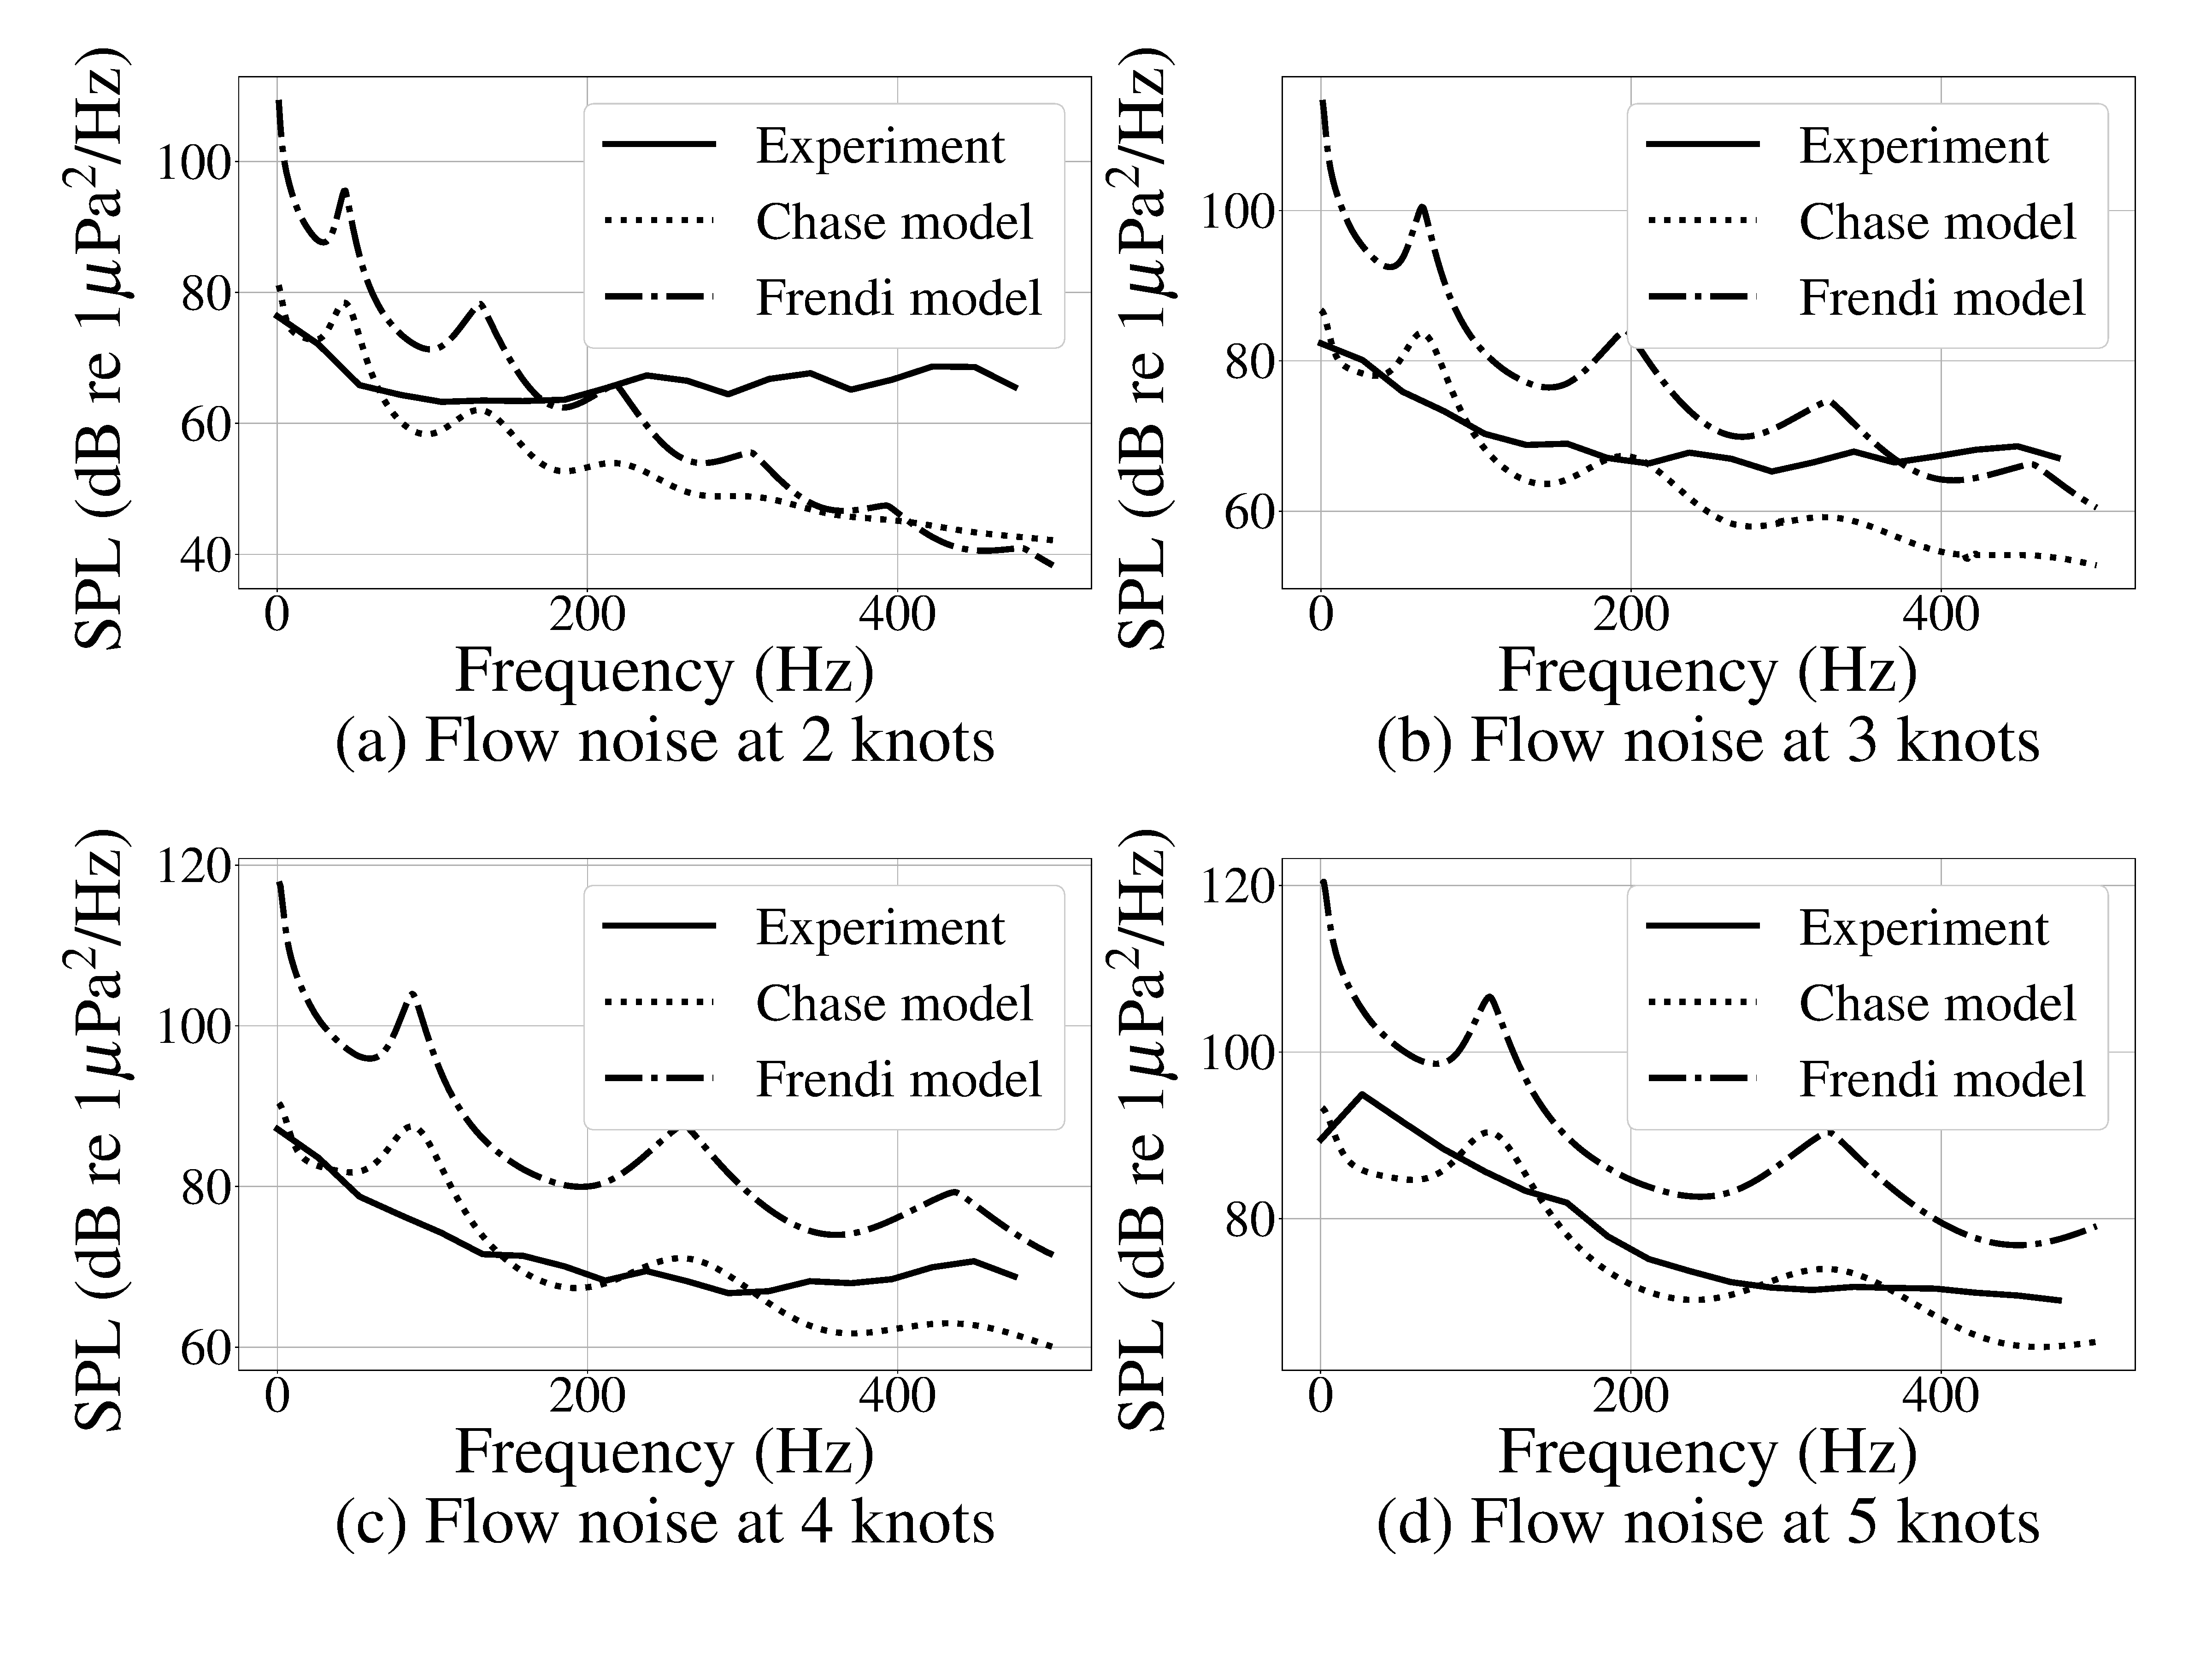
\includegraphics[width=4.5in]{Chase,frendi_vs_Unni_comparison.eps}}
    \caption{Comparison of flow noise predicted by Chase~\cite{Chase1981} and Frendi~\cite{frendi2020} models with the experimental results~\cite{Unni2011} at different tow speeds.}
    \label{Chase,frendi,expt}
\end{figure}
 
%%%%%%%%%%%%% end figure %%%%%%%%%%%%%%%%%%%%%%%%%%%%%%%%%%%%%%%%%%%%%%%%%%%%%%
Figure~\ref{Chase,frendi,expt} compares the flow noise estimated by the Chase~\cite{Chase1981} and Frendi~\cite{frendi2020} models with the experimental results~\cite{Unni2011} at various tow speeds for a solid cylinder having a diameter of 0.01~m. The sonar array consists of 66 hydrophones, each of length 8~mm, placed at the outer surface of the cylinder with an interval of 16~mm. It is evident from Fig.~\ref{Chase,frendi,expt} that the Frendi model consistently overestimates the flow noise at almost all frequencies and tow speeds, whereas the Chase model aligns well with experiments at high tow speeds. However, at low speeds, there is a significant difference between the Chase model and the experiment, especially at high frequencies. Regardless of tow speed, both models predict a significant reduction in flow noise with frequency compared to the experimental results. To address these differences, a new model of the turbulent pressure spectrum is proposed in this work to better match the experimental data, particularly at low tow speeds. The development of this new model is discussed in the following section.
%%%%%%%%%%%%%%%%%%%%%%%%%%%%%%%%%%%%%%%%%%%%%%%%%%%%%%%%%%%%%%%%%%%%%%%%%%%%%%%
\section{A new semi-empirical model of the turbulent pressure spectrum}\label{sec:hybmodel}
It is shown in the previous sections that the Chase and Frendi models show a significant deviation from the experimental results~\cite{Unni2011} at low tow speeds and at high frequencies. In this section, a new semi-empirical model of the turbulent pressure spectrum is developed that closely aligns with the experimental results~\cite{Unni2011}. This new model is derived using the insights from both the Chase and Frendi models and is referred to as the \textit{hybrid model}.

\subsection{The hybrid model}
In the \textit{hybrid model}, the pressure spectrum of the Chase model~\cite{Chase1981}~(Section~\ref{Chase model}) is used in conjunction with the exponential decay function present in the Frendi model~\cite{frendi2020}~(Section~\ref{Frendi model}). Accordingly, the turbulent pressure spectrum is given by
\begin{equation}\label{hybrid model equation}
    \Hat{p}(k_{z},k_{2},\omega) = C_{3}\Bar{P}(\omega)e^{-\Hat{\alpha}r_{k}}.
\end{equation}
In the above equation, the autospectrum $\Bar{P}(\omega)$ is given by
\begin{equation}\label{autospectrum equation}
    \Bar{P}(\omega) = \int^{\infty}_{-\infty}\Hat{p}_{0}(\omega,k_{z})dk_{z},
\end{equation}
where $\Hat{p}_{0}(\omega,k_{z})$ is the same as that used in the Chase model~(Eq.~(\ref{Turbulent pressure spectrum equation Chase})). In this new model, the wavenumber dependency is included in the form of an exponential function $e^{-\Hat{\alpha}r_{k}}$, where $\Hat{\alpha} = \alpha\delta$ with
\begin{equation}\label{alpha hybrid model}
   \alpha = \frac{a_1}{\pi}\frac{1}{\sqrt{1+a_2(\frac{\omega \delta}{u_{t}}-50)^{2}}},
\end{equation}
\begin{equation}
    \delta = [48Re_a^{-1}Re_x^{(0.0226\log{Re_a}+0.2478)}]^{\frac{1}{0.91}}
\end{equation}
and
\begin{equation}
    |{r_{k}}|^{2} = \bigg(k_{z} - \frac{\omega}{u_{c}}\bigg)^{2} + (mk_{2})^{2}.
\end{equation}
In Eq.~(\ref{alpha hybrid model}), $a_1$ and $a_2$ determine the behavior of the spectrum at low and high frequencies, respectively. It has been observed in Fig.~\ref{Chase,frendi,expt} that the predictions of the Frendi model deviate more at higher frequency ranges. Therefore, the value of $a_2$ is decreased from $3\times10^{-5}$ to $3\times10^{-6}$. Different values of $a_1$ and $C_3$ were tested to match the experimental results given in Fig.~\ref{Chase,frendi,expt}. A better match is found with the experimental data when $a_1 = 1$ and $C_3=1\times10^{-4}$. Furthermore, the turbulent pressure spectrum given in Eq.~(\ref{hybrid model equation}) is integrated over the cross-flow wavenumber $k_2$ from $-1/2R$ to $1/2R$ to obtain the pressure spectrum $\Hat{p}_0(k_z,\omega)$ for the axial flow past a solid cylinder~\cite{Chase1981}. 
Thus,
\begin{equation}\label{hybrid model turbulent pressure}
    \Hat{p}_0(k_{z},\omega) = \int_{-1/2R}^{1/2R}\Hat{p}(k_{z},k_{2},\omega)dk_{2}.
\end{equation}

The hybrid model is used to compute the flow noise for axial flow past a solid cylinder. The results of the new model and their comparison with the existing models and Unnikrishnan's experimental results~\cite{Unni2011} are presented in the next subsection.

\subsection{Flow noise}
The flow noise can be computed using Eq.~(\ref{Flow noise equaton from Unni}). Here, the turbulent pressure spectrum $\Hat{p}_0(k_z,\omega)$ for the new hybrid model is given by Eq.~(\ref{hybrid model turbulent pressure}) and the hydrophone response function $H(k_z)$ is given by Eq.~(\ref{Hydrophone response equation from Unni}).
%%%%%%%%%%%%%%%%%%%%%%%%%%%%%%%%%%%%%%%%
\begin{figure}[ht]
    \centerline{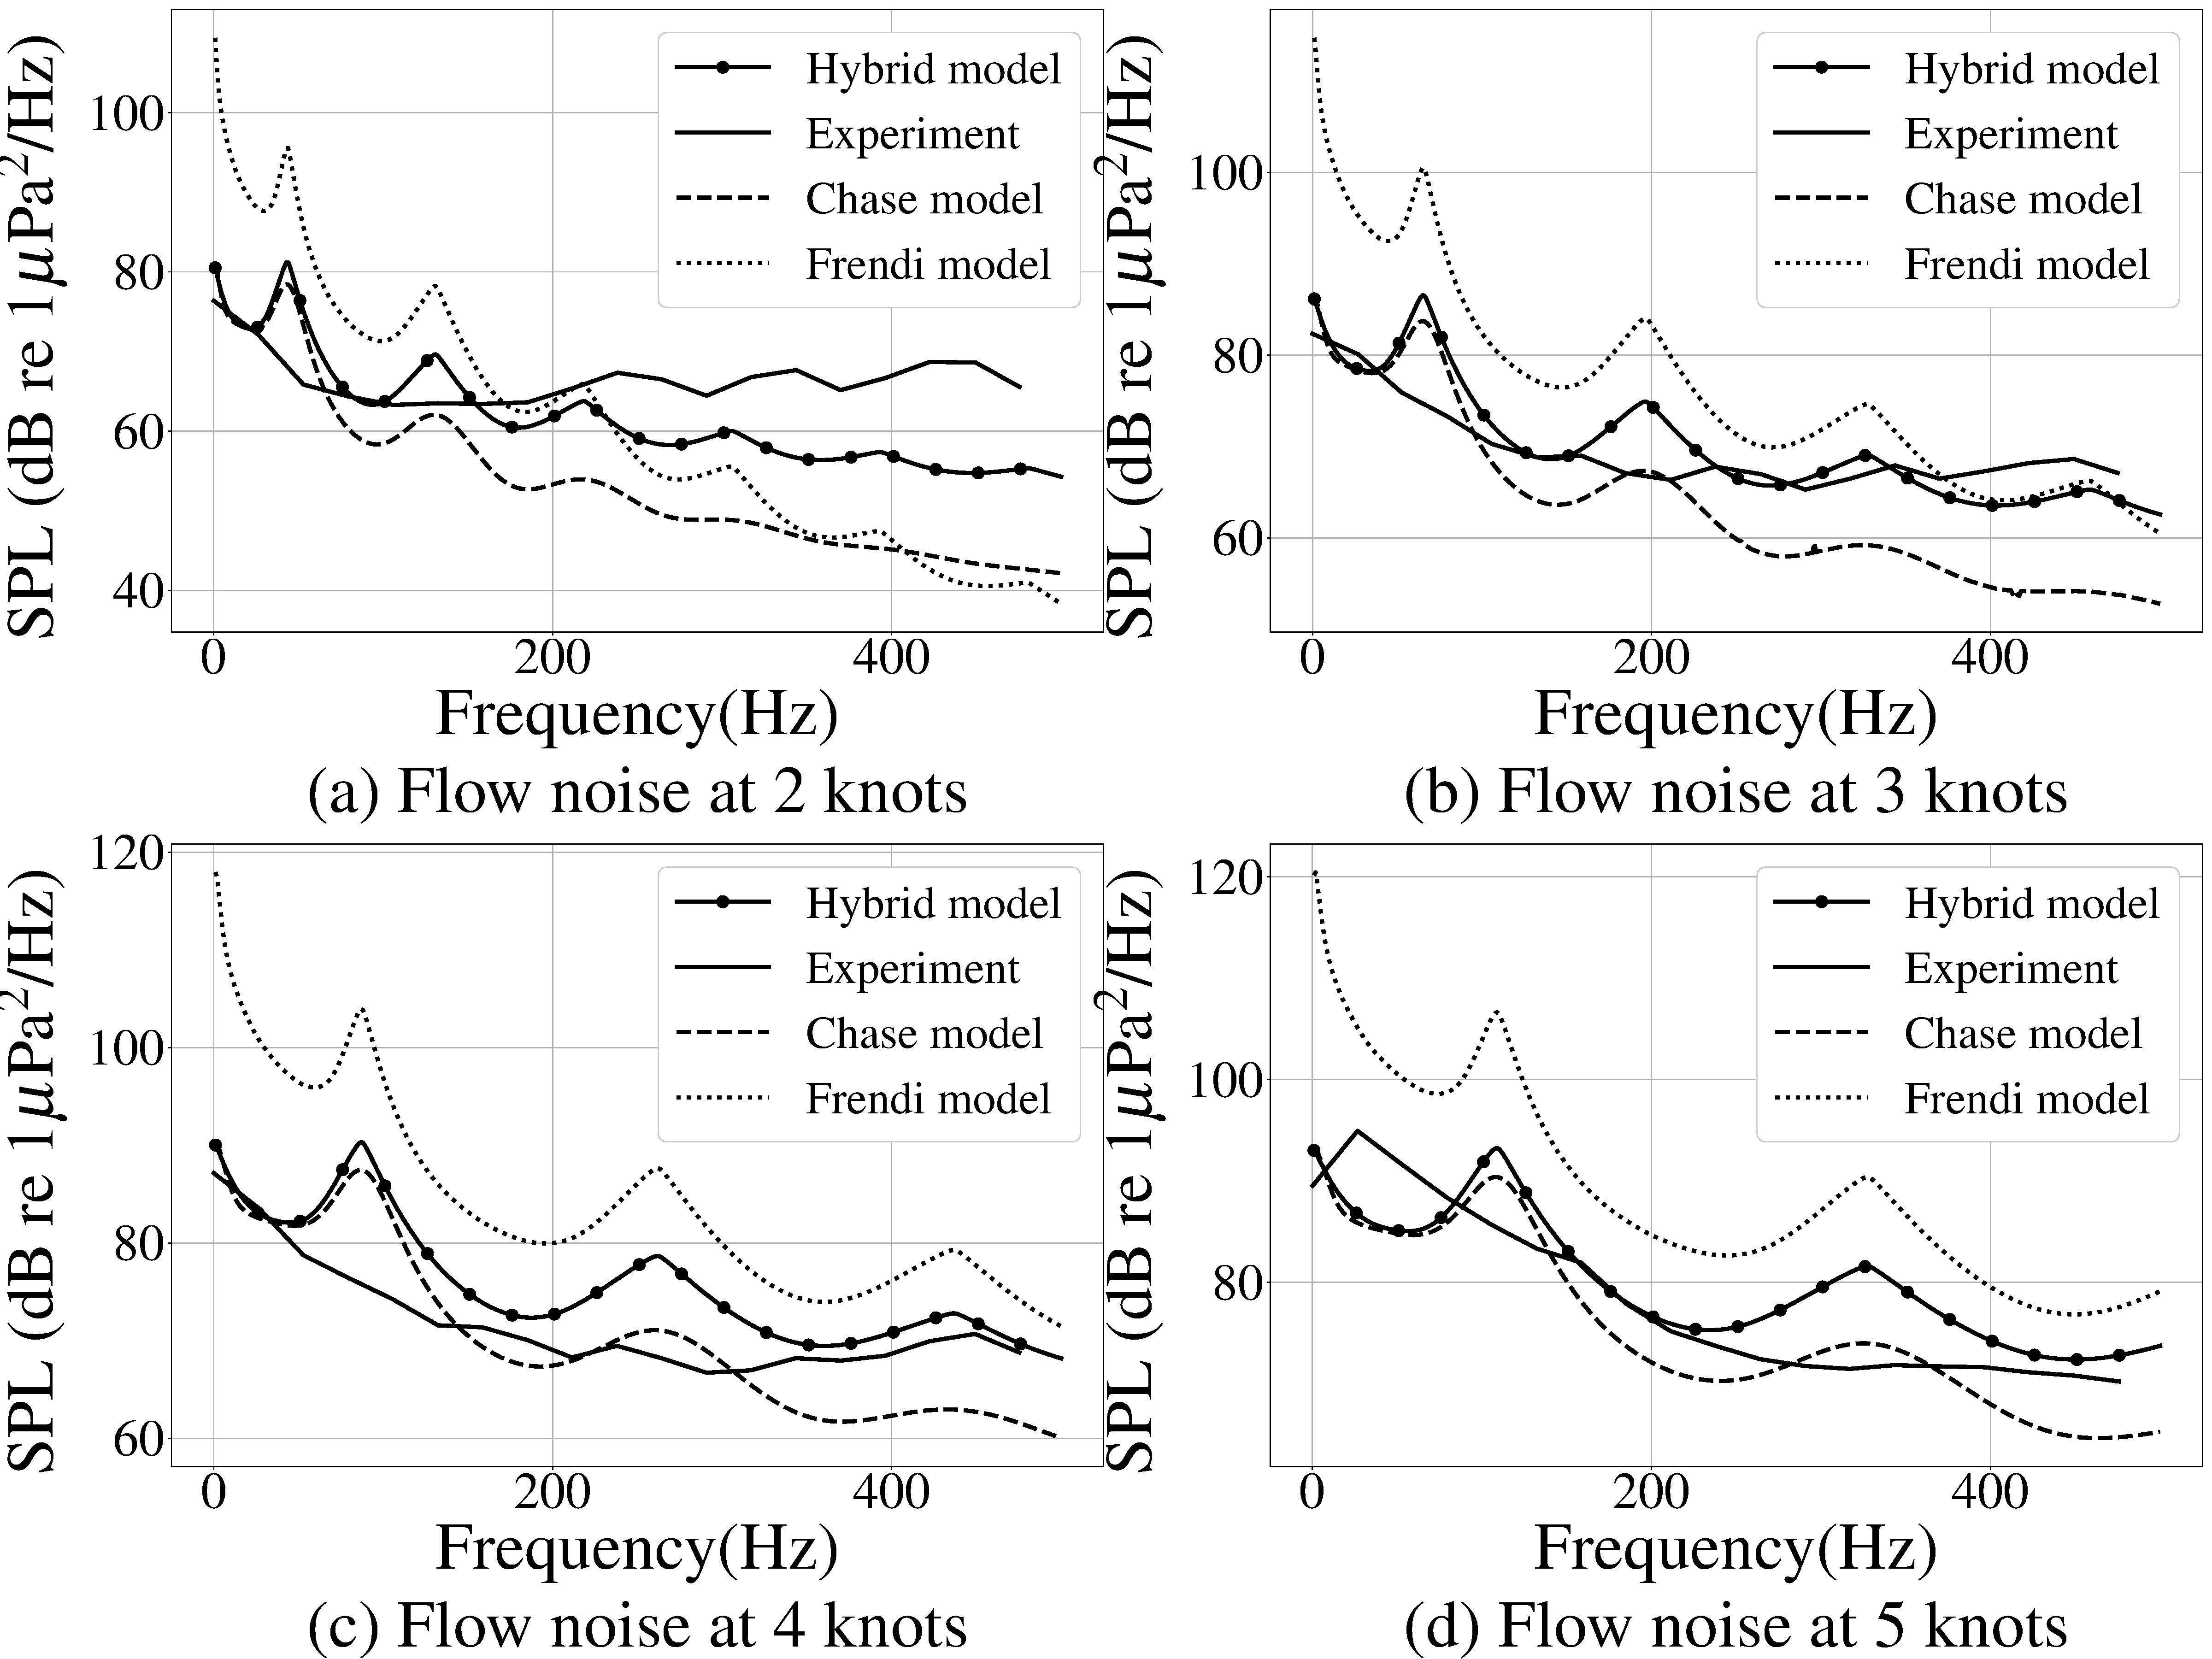
\includegraphics[width=4.5in]{Hybrid_model_Chase_frendi_vs_Unni_comparison.eps}}
    \caption{A comparison of flow noise predicted by the hybrid model, the Chase model~\cite{Chase1981} and Frendi model~\cite{frendi2020} with that measured from experiments~\cite{Unni2011} at different tow speeds.}
\label{fig:Flow_noise_of_Hybrid_model_with_chase_frendi_and_Unnikrishnan}
\end{figure}
%%%%%%%%%%%%%%%%%%%%%%%%%%%%%%%%%%%%%%%%
A comparison of flow noise measured in SPL (see Eq.~(\ref{SPL outside noise})) computed using the new hybrid model, Chase model~\cite{Chase1981} and Unnikrishnan's experiment~\cite{Unni2011} are shown in Fig.~\ref{fig:Flow_noise_of_Hybrid_model_with_chase_frendi_and_Unnikrishnan}. It can be seen that the predictions of the new hybrid model are consistent with the measured values~\cite{Unni2011} at all frequencies and towing speeds. Although the hybrid model underpredicts noise at high frequencies for the 2 knots case, the predictions are better than that by the existing Chase and Frendi models.


A comparison of the turbulent pressure spectrum $\Hat{p}_0(k_z,\omega)$ predicted by the hybrid model (Eqs.~(\ref{hybrid model equation})-(\ref{hybrid model turbulent pressure})), the Chase model~(Eq.~(\ref{Turbulent pressure spectrum equation Chase})) and the Frendi model~(Eq.~(\ref{One D equation Frendi})) for different frequencies at 2 knots is shown in Fig.~\ref{pressure comparison of hybrid model with chase and Frendi}. Here, the diameter of the cylinder is chosen as 10~mm, density of the fluid is 1000~kg/m$^3$ and the SPL is calculated at 11~m from the leading edge of the solid cylinder. 
%%%%%%%%%%%%%%%%%%%%%%%%%%%%%%%%%%%%%%%%%%%%%%%%%%%%%%%%%%%%%%%%%%%%%%%%%%%%%%%
\begin{figure}
    \centerline{
    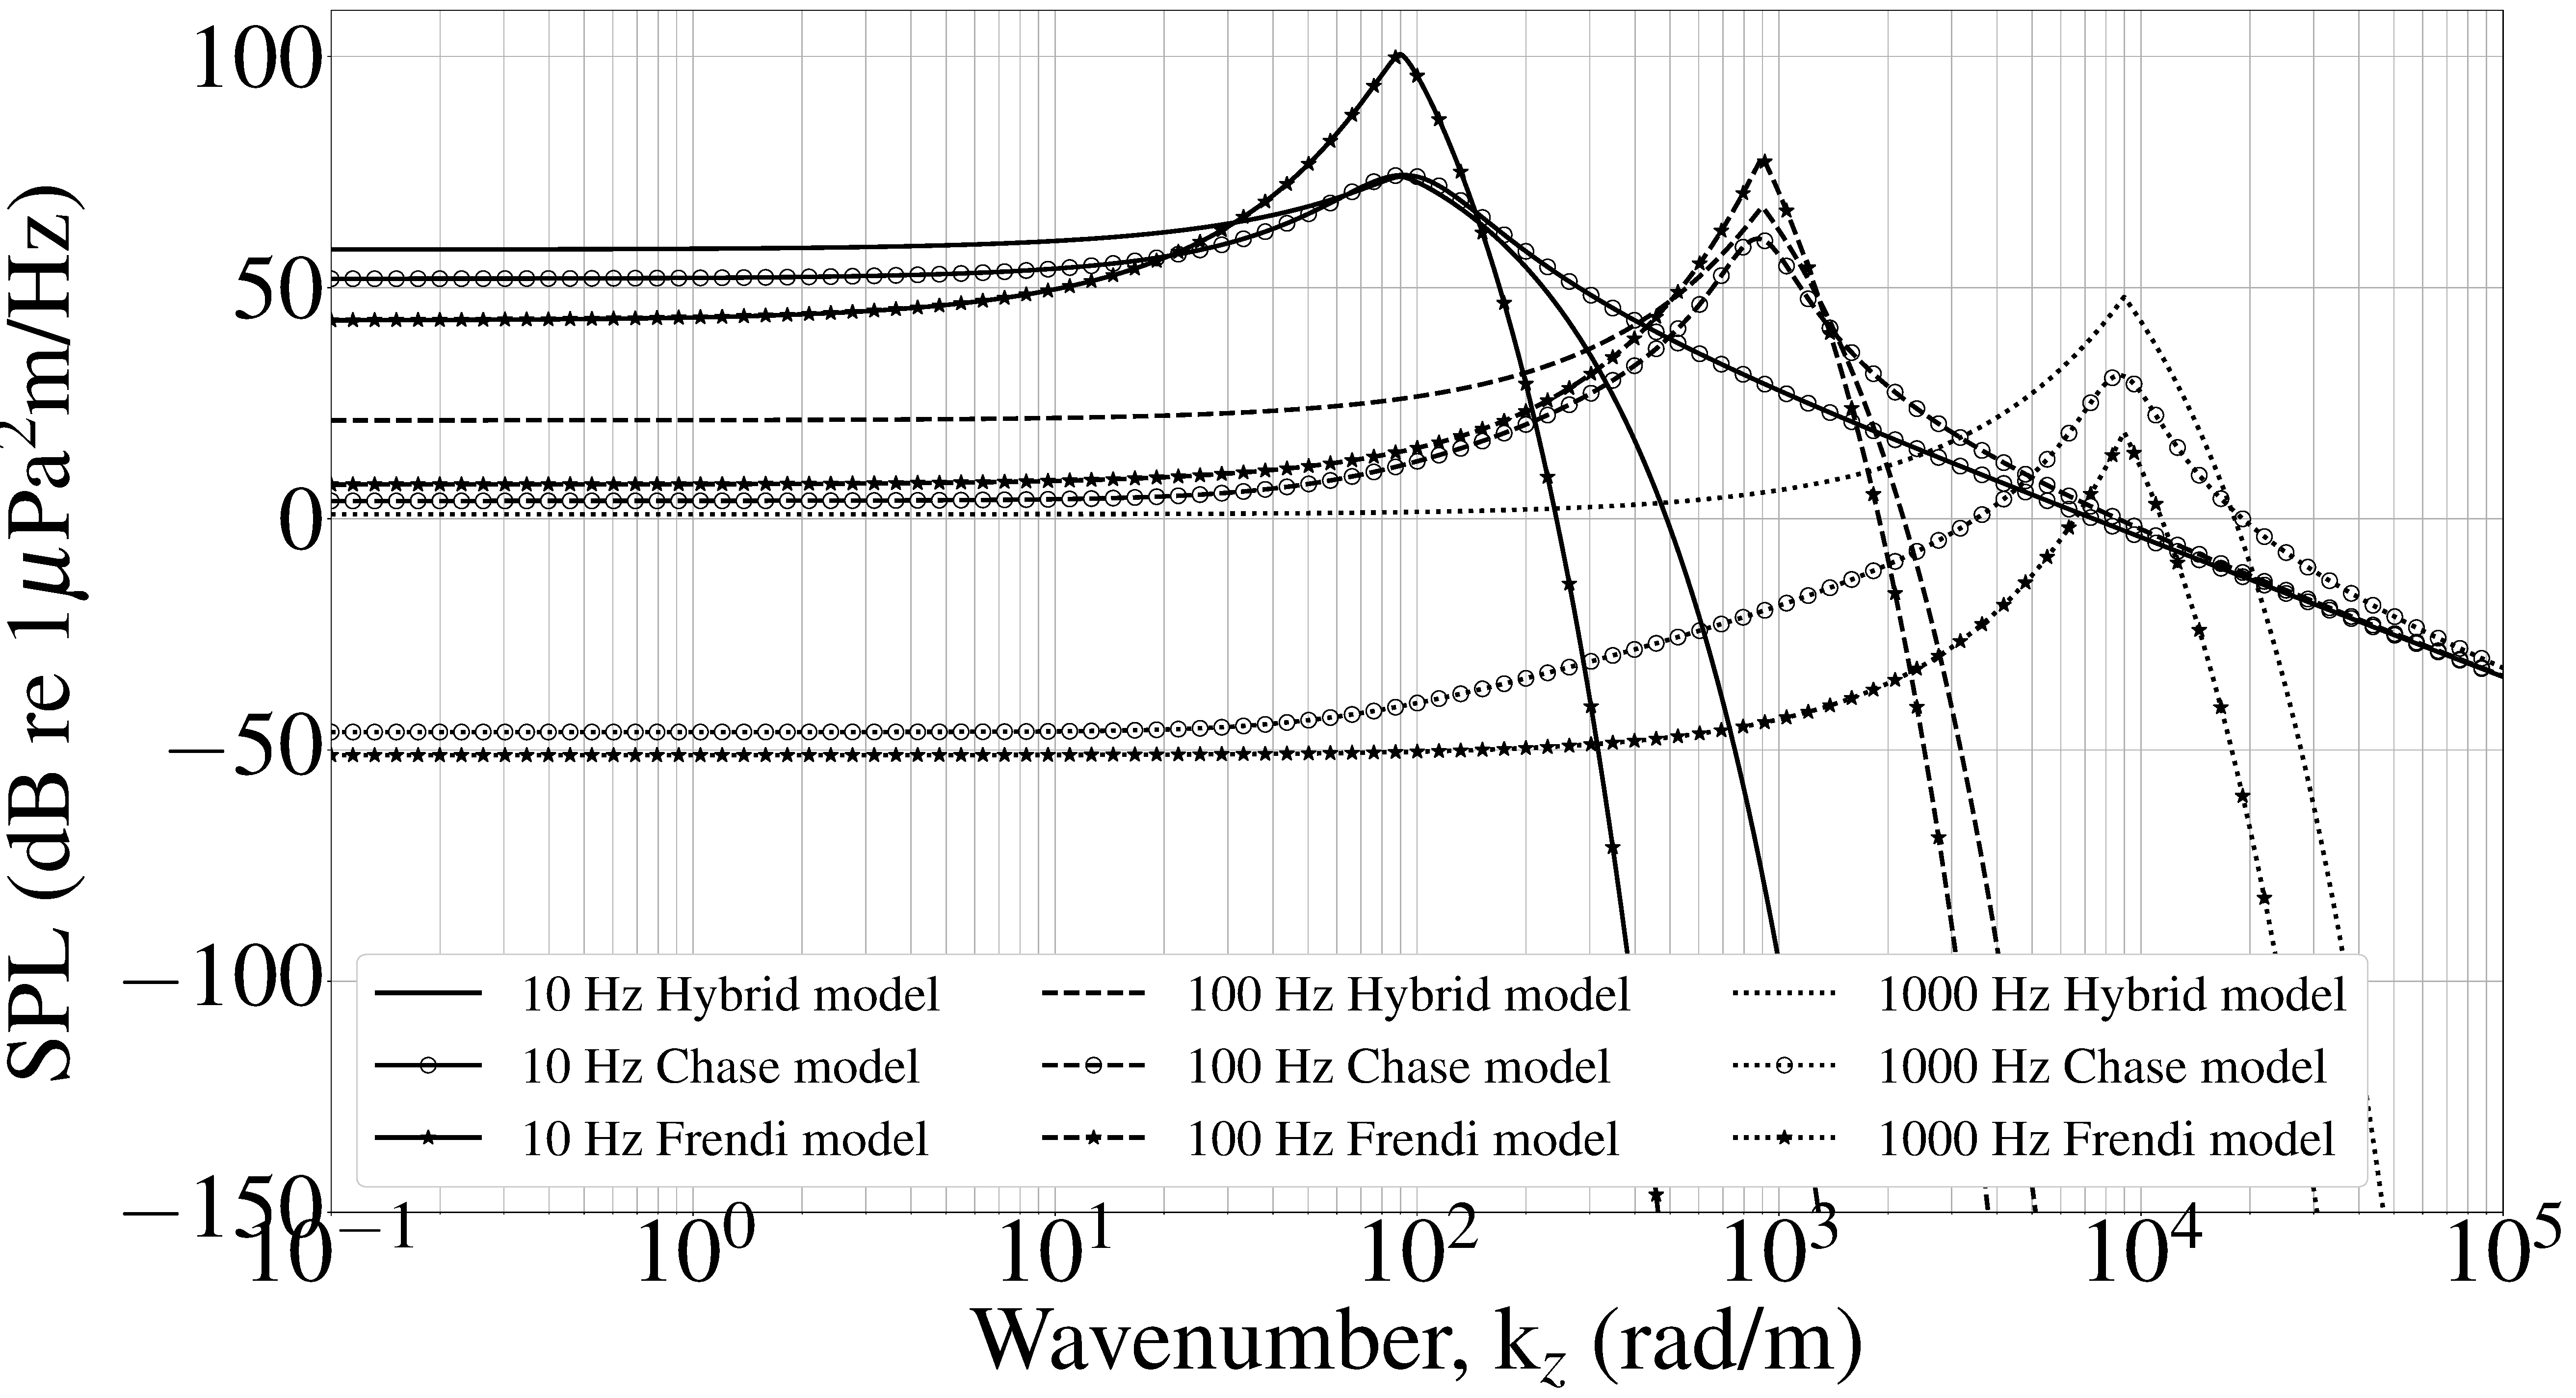
\includegraphics[width=4.3in]{Chase_hybrid_Frendi_outside_pressure_Spectrum.eps}}
    \caption{A comparison of the turbulent pressure spectrum $\Hat{p}_0(k_z,\omega)$ given by the hybrid model~(Eq.~(\ref{hybrid model turbulent pressure})), Chase~(Eq.~(\ref{Turbulent pressure spectrum equation Chase})) and Frendi~(Eq.~(\ref{One D equation Frendi})) model at 2~knots.}
    \label{pressure comparison of hybrid model with chase and Frendi}
\end{figure}
%%%%%%%%%%%%%%%%%%%%%%%%%%%%%%%%%%%%%%%%%%%%%%%%%%%%%%%%%%%%%%%%%
It can be seen from Fig.~\ref{pressure comparison of hybrid model with chase and Frendi} that for a given frequency, at low wavenumbers, the turbulent pressure spectrum increases at a slow rate. It peaks at convective wavenumber $k_c$~($=\omega/u_c$) forming a convective ridge. It can be seen that while all the models predict a `flat' spectrum at lower wavenumbers and a ridge at convective wavenumber, their predictions differ significantly at large wavenumbers. The presence of an exponential function results in an exponential decrease in the spectrum at large wavenumbers for the hybrid and Frendi models. Chase model predicts a higher spectrum with a smaller slope at large wavenumbers. It can be seen from Fig.~\ref{pressure comparison of hybrid model with chase and Frendi} that the predictions by the three models are closer at lower frequencies. However, at high frequencies, the hybrid model predicts a spectrum that is higher than the rest. This difference in the spectrum predicted by the hybrid model helps to achieve closer agreement with the measured flow noise, as shown in Fig.~\ref{fig:Flow_noise_of_Hybrid_model_with_chase_frendi_and_Unnikrishnan}
%%%%%%%%%%%%%%%%%%%%%%%%%%%%%%%%%%%%%%%%%%%%%%%
\subsection{Non-dimensional power spectral density}
The non-dimensional power spectral density, $Q_{ND}$, of the flow noise is defined as
\begin{equation}
    Q_{ND} = \frac{Q(\omega)}{\rho^2 D U^3},
\end{equation}
where $Q(\omega)$ is the flow noise given by Eq.~(\ref{Flow noise equaton from Unni}) and $D$ is the cylinder diameter. The non-dimensional power spectral density calculated using the hybrid model (Eqs.~(\ref{hybrid model equation})-(\ref{hybrid model turbulent pressure})) at different tow speeds are shown in Fig.~\ref{non dimensional plot of hybrid model}.

It can be seen that, the non-dimensional power spectral density for different tow speeds collapse to a single curve against the non-dimensional frequency $\omega D/u$. One can therefore obtain the power spectral density at different tow speeds and cylinder diameters using this ``single'' non-dimensional curve.


While developing a new model of turbulent pressure field for axial flow past a solid cylinder, it is assumed that the cylinder is rigid and therefore the pressure field is not altered by the cylinder displacement field. However, the cylindrical tube in towed sonar arrays is not rigid and can be assumed to be elastic. The turbulent pressure fluctuation outside the elastic tube, creates vibration inside the tube and in turn generates acoustic waves in the fluid inside the tube. The following section presents a three-dimensional vibroacoustic model of a fluid-filled elastic tube, which is further used with the new hybrid model of the external turbulent pressure excitation to estimate on-axis flow noise.

\begin{figure}
    \centerline{
    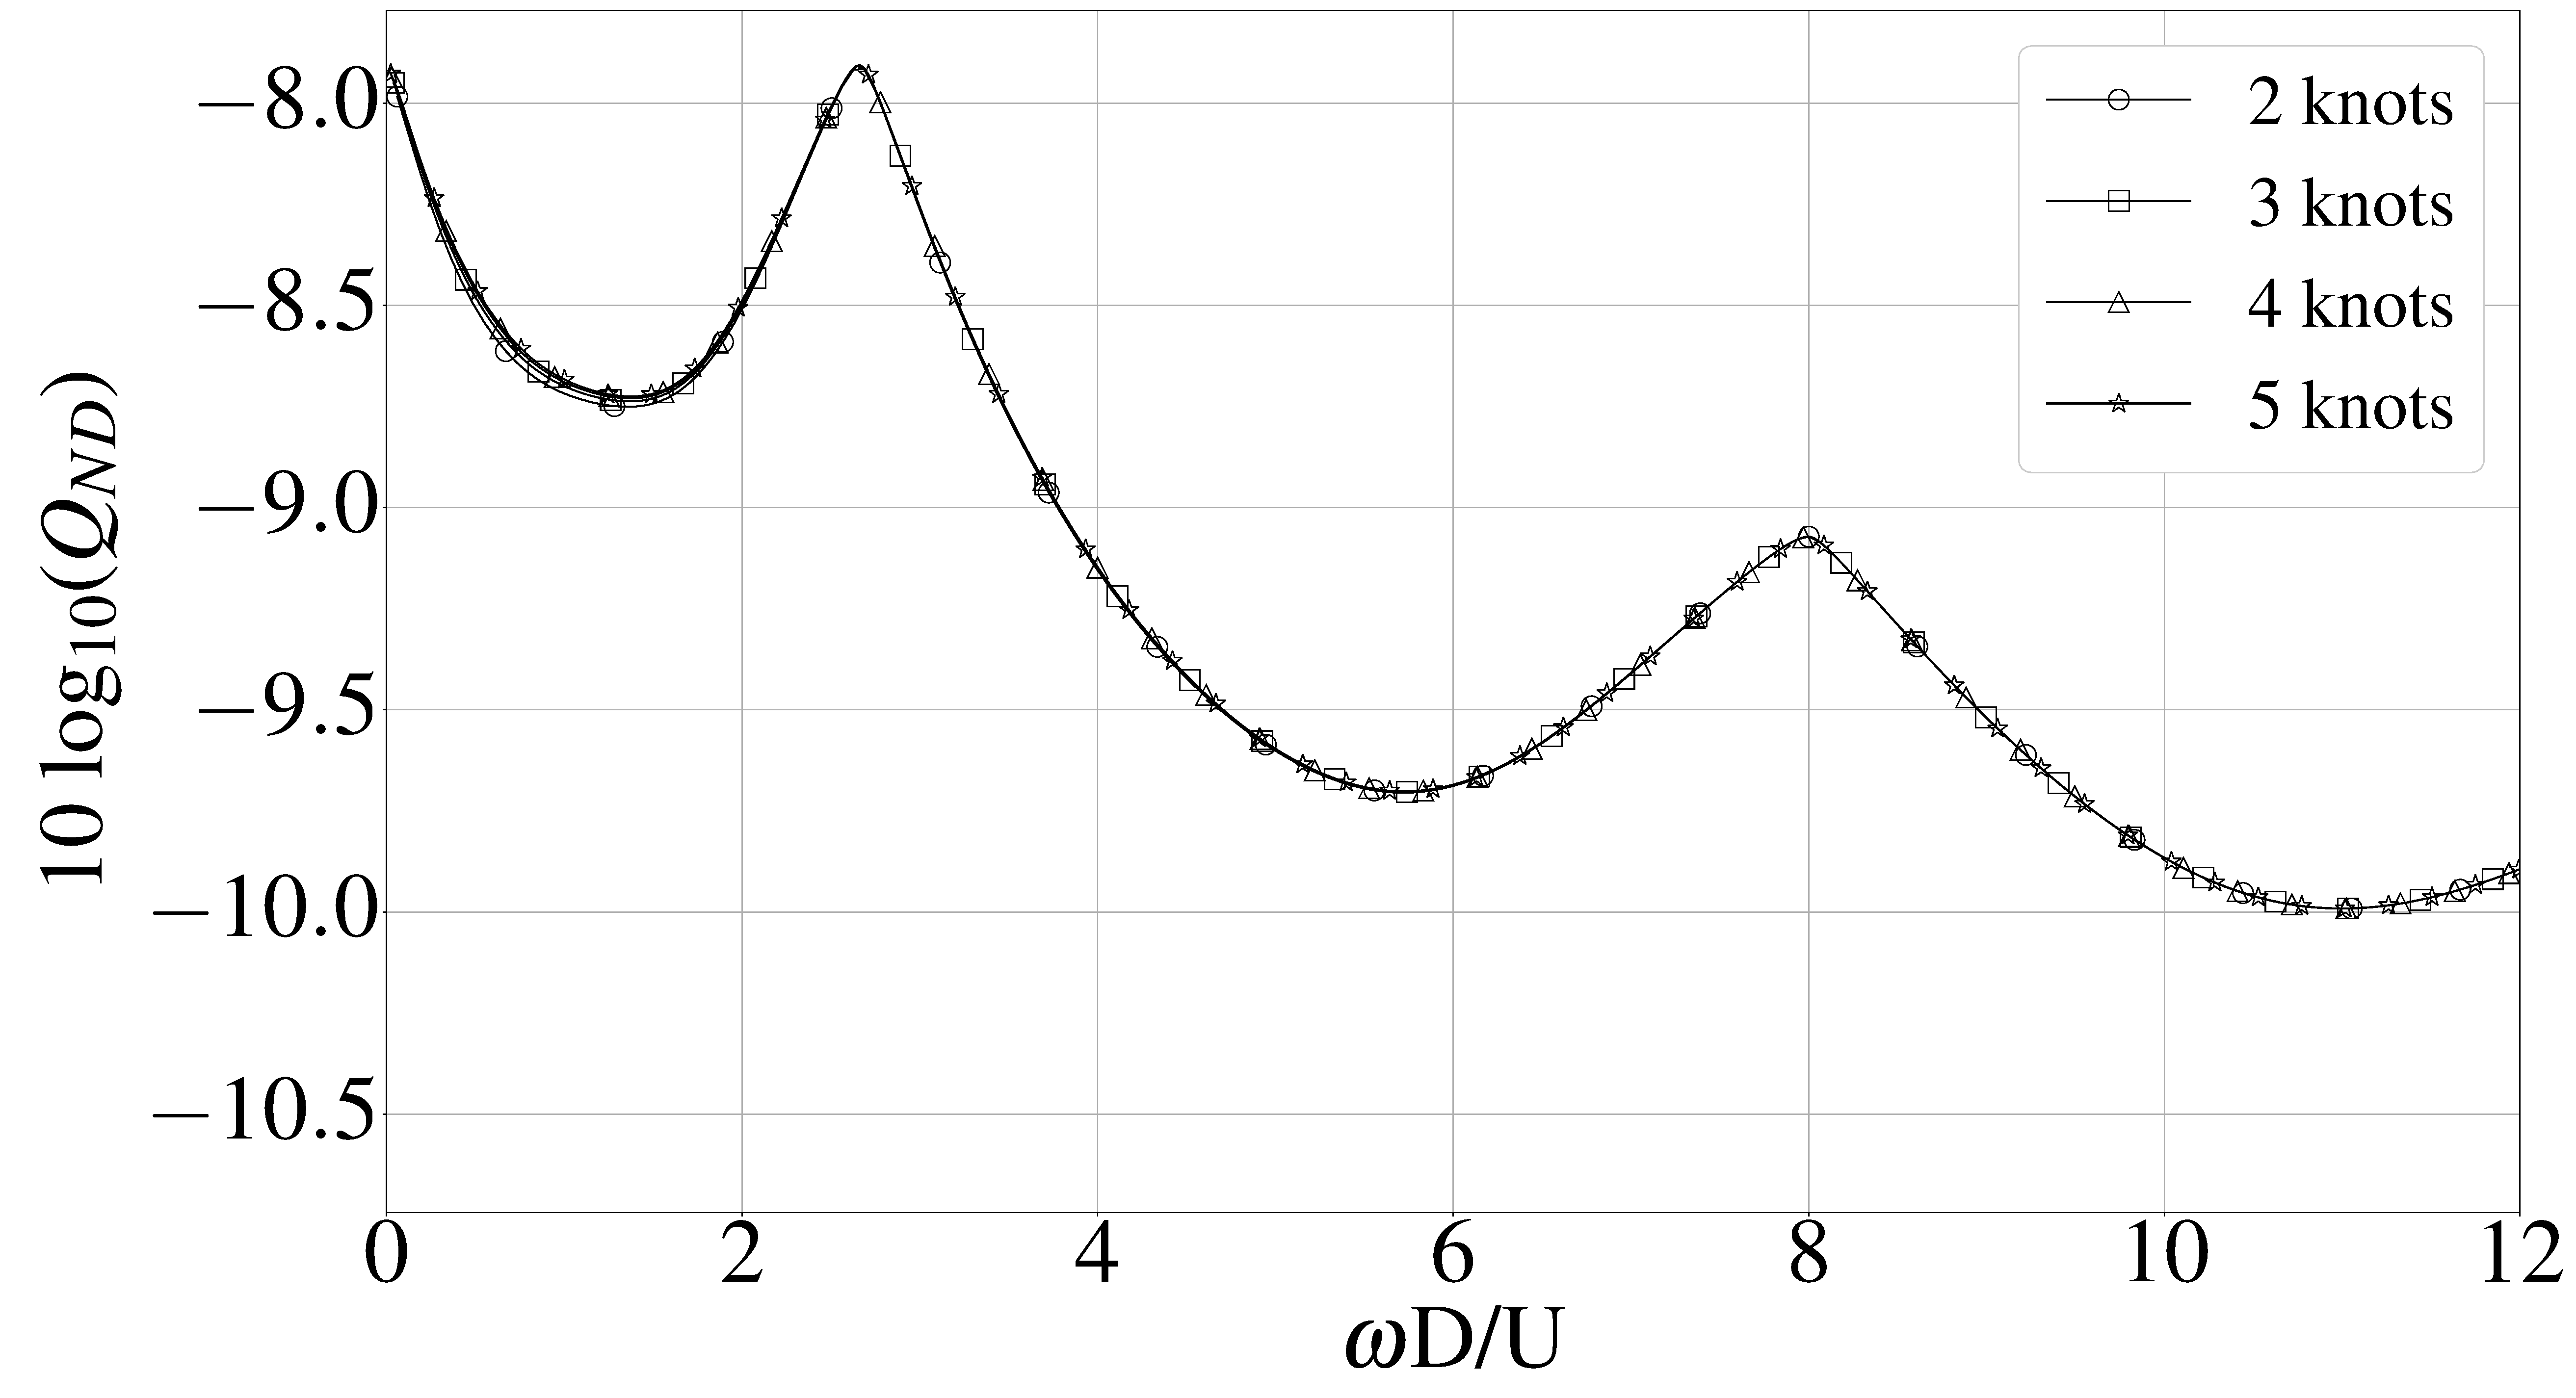
\includegraphics[width=4.3in]{Non_dimensional_plot_of_hybrid_model.eps}}
    \caption{Non-dimensional power spectral density for different tow speeds using the new hybrid model.}
    \label{non dimensional plot of hybrid model}
\end{figure}

%%%%%%%%%%%%%%%%%%%%%%%%%%%%%%%%%%%%%%%%%%%%%%%%%%%%%%%%%%%%%%%%%%%%%%

\section{Three-dimensional vibroacoustic (3D-VA) model of a fluid-filled elastic tube} \label{sec:vamodel}
This section develops a fully-coupled three-dimensional vibroacoustic (3D-VA) model of the fluid-filled elastic tube. A schematic of the fluid-filled tube is shown in Fig.~\ref{fig:fluid filled elastic tube}. First, the displacement field of the elastic tube is derived from the Navier-Lame equilibrium equation (see Section~\ref{governing equation for 3d cylinder}) and then the acoustic pressure field inside the tube is derived from the acoustic wave equation (see Section~\ref{inside fluid modelling}). The structure (elastic tube) and the fluid (interior fluid) are then coupled with the help of stress and displacement boundary conditions at the interface (see Section~\ref{BCS}). External pressure excitation is also taken into account in the form of a stress boundary condition on the outer surface of the tube. The boundary conditions, when expressed in terms of the unknown displacement and pressure fields, form a system of linear algebraic equations. The unknown displacement and pressure fields are then calculated by solving this system of equations (see Section~\ref{solution methods}).

\begin{figure}
    \centerline{
    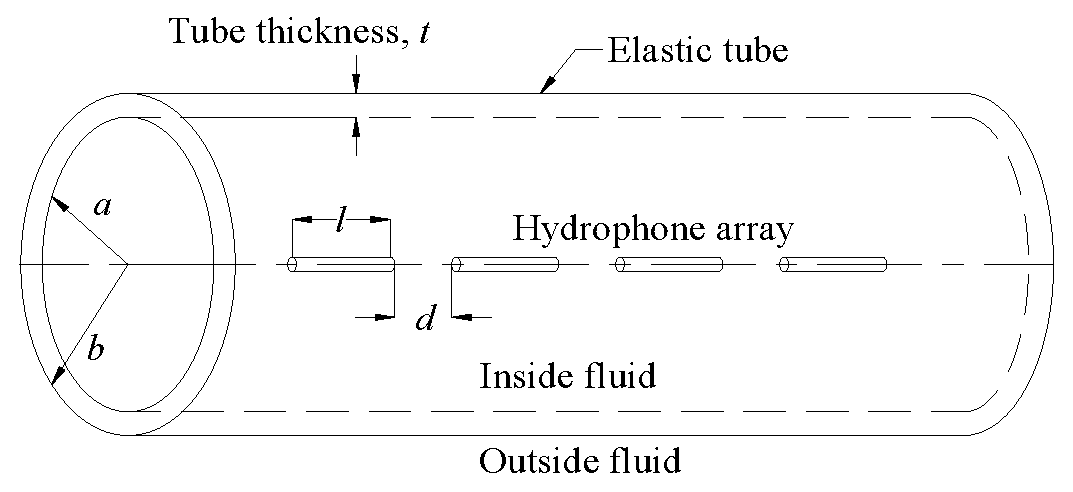
\includegraphics[width=4.3in]{Sonar_array_element.eps}}
     \caption{Fluid filled elastic tube.}
    \label{fig:fluid filled elastic tube}
\end{figure}

%%%%%%%%%%%%%%%%%%%%%%%%%%%%%%%%%%%%%%%%%%%%

\subsection{The elastic tube displacement and stress fields}\label{governing equation for 3d cylinder}
This section involves modeling of an elastic tube using the Navier-Lame equilibrium equation in three-dimensional cylindrical coordinates. The Navier-Lame equilibrium equation is given by~\cite{Martin2014}
\begin{equation}\label{Navier equation of motion 3d}
    \mu\nabla^{2}\mathbf{U}(r,\theta,z,t)+(\lambda+\mu)\pmb{\nabla}\pmb{\nabla}.\mathbf{U}(r,\theta,z,t) = \rho_s\mathbf{\ddot{U}}(r,\theta,z,t),
\end{equation}
where $\mathbf{U}$ is the displacement vector ($= \{W_e, \Theta_e, U_e\}^T$, $W_e$ represents the radial, $\Theta_e$ represents the azimuthal and $U_e$, the axial displacement fields), $\lambda$ and $\mu$ are the Lame's coefficients, $\rho_s$ is the density of the tube and $\pmb{\nabla}$ is the gradient operator in three dimension given by
\begin{equation}\label{del operator}
    \pmb{\nabla} = \frac{\partial}{\partial r}{\mathbf{e_r}} + \frac{1}{r}\frac{\partial}{\partial \theta}\mathbf{e}_{\pmb{\theta}} + \frac{\partial}{\partial z}\mathbf{e_z}.
\end{equation}
The displacement vector $\mathbf{U}$ may be represented using the Helmholtz decomposition method as
 \begin{equation}\label{Helmholtz equation 3d}
    \mathbf{U} = \pmb{\nabla}\phi+\pmb{\nabla}\times\pmb{\psi},
\end{equation}
where $\phi$ is a scalar potential and $\pmb{\psi}$ is a vector potential. 
The scalar and vector potential functions satisfy the Navier-Lame equation for $n=0$ and for all positive integer values of $n$. A complete solution to Navier-Lame equation can be obtained as
\begin{equation}\label{Scalar potential equation}
    \phi(r,\theta,z,t) = \sum_{n=0}^{\infty}\left[A_{1}J_{n}(\beta_1 r) + A_{2}Y_{n}(\beta_1 r)\right]\\ \left[A_{3}\cos(n\theta) + A_{4}\sin(n\theta)\right]\mathbf{e}^{i(k_{z}z-\omega t)},
\end{equation}
\begin{equation}\label{Vector potential equation r}
    \psi_{r}(r,\theta,z,t) = \sum_{n=0}^{\infty}\left[C_{1}J_{n+1}(\beta_2r) + C_{2}Y_{n+1}(\beta_2 r)\right]\\\sin(n\theta)\mathbf{e}^{i(k_{z}z-\omega t)},
\end{equation}
\begin{equation}\label{Vector potential equation theta}
    \psi_{\theta}(r,\theta,z,t) = \sum_{n=0}^{\infty}-\left[C_{1}J_{n+1}(\beta_2 r) + C_{2}Y_{n+1}(\beta_2 r)\right]\\\cos(n\theta)\mathbf{e}^{i(k_{z}z-\omega t)}
\end{equation}
and
\begin{equation}\label{Vector potential equation z}
    \psi_{z}(r,\theta,z,t) = \sum_{n=0}^{\infty}\left[B_{1}J_{n}(\beta_2 r) + B_{2}Y_{n}(\beta_2 r)\right]\\ \left[B_{3}\cos(n\theta) + B_{4}\sin(n\theta)\right]\mathbf{e}^{i(k_{z}z-\omega t)}
\end{equation}
In this work, the above expressions are truncated to only $n=0$ and $n=1$ terms and further used to compute the elastic tube displacement and stress fields. A detailed derivation of the potential functions are given in Section~S1 of the Supplimental material.
\allowdisplaybreaks
%%%%%%%%%%%%%%%%%%%%%%%%%%%%%%%%%%%%%%%%%%%%%%%%%%%%%%%%%%%%%%%%%%%%%%
\subsubsection{Elastic tube displacement components}
In this subsection, the displacement components of the elastic tube in radial ($W_e$), azimuthal ($\Theta_e$) and axial ($U_e$) directions, are derived. The displacement components are given by Eq.~(\ref{Helmholtz equation 3d}).
\begin{equation}
    W_{e}(r,\theta,z,t) = \frac{\partial\phi}{\partial r} + \frac{1}{r}\frac{\partial\psi_{z}}{\partial\theta} - \frac{\partial\psi_{\theta}}{\partial z},
\end{equation}
\begin{equation}
    \Theta_e(r,\theta,z,t) = \frac{1}{r}\frac{\partial\phi}{\partial\theta} + \frac{\partial\psi_r}{\partial z} - \frac{\partial\psi_z}{\partial r}
\end{equation}
and
\begin{equation}
    U_{e}(r,\theta,z,t) = \frac{\partial\phi}{\partial r} + \frac{1}{r}\frac{\partial\psi_{z}}{\partial\theta} - \frac{\partial\psi_{\theta}}{\partial z}
\end{equation}
Substituting for the scalar (Eq.~(\ref{Scalar potential equation})) and the vector potential (Eqs.~(\ref{Vector potential equation r}) - (\ref{Vector potential equation z})) functions, the radial displacement field is
\begin{multline}
    W_e(r,\theta,z,t) =\\ \mathbf{e}^{i(k_{z}z-\omega t)}\bigg\{\frac{1}{r}[r\beta_1 J_0(r\beta_1)\cos(\theta) - J_1(r\beta_1)(\cos(\theta) + r\beta_1)]E_1 + \frac{1}{r}\sin(\theta)[r\beta_1 J_0(r\beta_1)\\ - J_1(r\beta_1)]E_2 + \frac{1}{r}[r\beta_1 Y_0(r\beta_1)\cos(\theta) - Y_1(r\beta_1)(\cos(\theta) + r\beta_1)]F_1 + \frac{1}{r}\sin(\theta)[r\beta_1 Y_0(r\beta_1)\\ - Y_1(r\beta_1)]F_2 + ik_z[J_1(r\beta_2) + J_2(r\beta_2)\cos(\theta)]G_1 + ik_z[J_1(r\beta_2) + J_2(r\beta_2)\cos(\theta)]G_2\\ + [\frac{1}{r}J_1(r\beta_2)\cos(\theta)]H_1 + [\frac{1}{r}Y_1(r\beta_2)\cos(\theta)]H_2 - [\frac{1}{r}J_1(r\beta_2)\sin(\theta)]I_1 - [\frac{1}{r}Y_1(r\beta_2)\sin(\theta)]I_2 \bigg\},
\end{multline}
where, $E_1$, $E_2$, $F_1$, $F_2$, $G_1$, $G_2$, $H_1$, $H_2$, $I_1$ and $I_2$ are unknown constants with $E_1 = A_1A_3$, $E_2 = A_1A_4$, $F_1 = A_2A_3$, $F_2 = A_2A_4$, $G_1 = C_1$, $G_2 = C_2$, $H_1 = B_1B_4$, $H_2 = B_2B_4$, $I_1 = B_1B_3$ and $I_2 = B_2B_3$. The azimuthal displacement field is
\begin{multline}
    \Theta_e(r,\theta,z,t) =\\ \mathbf{e}^{i(k_{z}z-\omega t)}\bigg\{\frac{-1}{r}[J_1(r\beta_1)\sin(\theta)]E_1 + \frac{1}{r}[J_1(r\beta_1)\cos(\theta)]E_2 + \frac{-1}{r}[Y_1(r\beta_1)\sin(\theta)]F_1\\ + \frac{1}{r}[Y_1(r\beta_1)\cos(\theta)]F_2 + [ik_zJ_2(r\beta_2)\sin(\theta)]G_1 + [ik_zY_2(r\beta_2)\sin(\theta)]G_2\\ - \frac{\beta_2\sin(\theta)}{2}[J_0(r\beta_2)-J_2(r\beta_2)]H_1 - \frac{\beta_2\sin(\theta)}{2}[Y_0(r\beta_2)-Y_2(r\beta_2)]H_2\\ + \frac{1}{r}\{-r\beta_2J_0(r\beta_2)\cos(\theta) + J_1(r\beta_2)[r\beta_2+\cos(\theta)]\}I_1 + \frac{1}{r}\{-r\beta_2Y_0(r\beta_2)\cos(\theta)\\ + Y_1(r\beta_2)[r\beta_2+\cos(\theta)]\}I_2\bigg\}.
\end{multline}
The axial displacement field is
\begin{multline}
    U_e(r,\theta,z,t) =\\ \mathbf{e}^{i(k_{z}z-\omega t)}\bigg\{ik_z[J_{0}(r\beta_1) + J_{1}(r\beta_1)\cos(\theta)]E_1 + [ik_zJ_{1}(r\beta_1)\sin(\theta)]E_2\\ +  ik_z[Y_{0}(r\beta_1) + Y_{1}(r\beta_1)\cos(\theta)]F_1 +[ik_zY_{1}(r\beta_1)\sin(\theta)]F_2 \\
    - \beta_2[J_{0}(r\beta_2) + J_{1}(r\beta_2)\cos(\theta)]G_1 - \beta_2[Y_{0}(r\beta_2) + Y_{1}(r\beta_2)\cos(\theta)]G_2\bigg\}.
\end{multline}
The spatio-temporal ($r, \theta, z, t$) displacement field is then transformed to the wavenumber-frequency ($r, \theta, k_z, \omega$) domain using the Fourier transform pairs,
\begin{align}\label{Forward fourier transform}
    &\Hat{G}(r,\theta,k_{z},\omega) = \frac{1}{4\pi^{2}}\int^{\infty}_{-\infty}\int^{\infty}_{-\infty}g(r,\theta,z,t)e^{-i(k_{z}z-\omega t)}dzdt,\\
	\text{and}\nonumber \\
    &g(r,\theta,z,t) = \int^{\infty}_{-\infty}\int^{\infty}_{-\infty}\Hat{G}(r,\theta,k_{z},\omega)\mathbf{e}^{i(k_{z}z-\omega t)}dk_{z}d\omega\label{Backward fourier transform}.
\end{align} 
The transformed displacement components are given below.
\begin{enumerate}[label=(\alph*)]
    \item Radial displacement:
    \begin{multline}\label{Radial displacement 3d}
    \Hat{W}_{e}(r,\theta,k_z,\omega) = \Bigg\{\frac{-\chi_1}{2}\{2J_1(r\beta_1) + [J_2(r\beta_1) - J_0(r\beta_1)]\cos(\theta)\}\Bigg\}\Hat{P}_1(k_z,\omega)\\ + \Bigg\{\frac{\chi_1}{2}[J_0(r\beta_1) - J_2(r\beta1)]\sin(\theta)\Bigg\}\Hat{P}_2(k_z,\omega) + \Bigg\{\frac{-\chi_1}{2}\{2Y_1(r\beta_1)\\ + [Y_2(r\beta_1)-Y_0(r\beta_1)]\cos(\theta)\}\Bigg\}\Hat{Q}_1(k_z,\omega) + \Bigg\{\frac{\chi_1}{2}[Y_0(r\beta_1)-Y_2(r\beta1)]\sin(\theta)\Bigg\}\Hat{Q}_2(k_z,\omega)\\ - \Bigg\{\chi_2[J_1(r\beta_2)+J_2(r\beta_2)\cos(\theta)]\Bigg\}\Hat{R}_1(k_z,\omega) - \Bigg\{\chi_2[Y_1(r\beta_2) + Y_2(r\beta_2)\cos(\theta)]\Bigg\}\Hat{R}_2(k_z,\omega)\\ + \Bigg\{\frac{1}{r}[J_1(r\beta_2)\cos(\theta)]\Bigg\}\Hat{S}_1(k_z,\omega) + \Bigg\{\frac{1}{r}[Y_1(r\beta_2)\cos(\theta)]\Bigg\}\Hat{S}_2(k_z,\omega)\\ + \Bigg\{\frac{1}{r}[J_1(r\beta_2)\sin(\theta)]\Bigg\}\Hat{T}_1(k_z,\omega) + \Bigg\{\frac{1}{r}[Y_1(r\beta_2)\sin(\theta)]\Bigg\}\Hat{T}_2(k_z,\omega),
    \end{multline}
    where $\Hat{P}_1(k_z,\omega)$, $\Hat{P}_2(k_z,\omega)$, $\Hat{Q}_1(k_z,\omega)$, $\Hat{Q}_2(k_z,\omega)$, $\Hat{R}_1(k_z,\omega)$, $\Hat{R}_2(k_z,\omega)$, $\Hat{S}_1(k_z,\omega)$, $\Hat{S}_2(k_z,\omega)$, $\Hat{T}_1(k_z,\omega)$ and $\Hat{T}_2(k_z,\omega)$ are the unknown variables and $\chi_{1} = \frac{\beta_1}{jk_z}$ and $\chi_{2} =\frac{jk_z}{\beta_2}$.
    \item Azimuthal displacement:
    \begin{multline}\label{Azimuthal displacement 3d}
    \Hat{\Theta}_e(r,\theta,k_z,\omega) = \Bigg\{\frac{-\chi_1}{r\beta_1}[J_1(r\beta_1)\sin(\theta)]\Bigg\}\Hat{P}_1(k_z,\omega) + \Bigg\{\frac{\chi_1}{r\beta_1}[J_1(r\beta_1)\cos(\theta)]\Bigg\}\Hat{P}_2(k_z,\omega)\\ + \Bigg\{\frac{-\chi_1}{r\beta_1}[Y_1(r\beta_1)\sin(\theta)]\Bigg\}\Hat{Q}_1(k_z,\omega) + \Bigg\{\frac{\chi_1}{r\beta_1}[Y_1(r\beta_1)\cos(\theta)]\Bigg\}\Hat{Q}_2(k_z,\omega)\\ - \Bigg\{\chi_2J_2(r\beta_2)\sin(\theta)\Bigg\}\Hat{R}_1(k_z,\omega) - \Bigg\{\chi_2Y_2(r\beta_2)\sin(\theta)\Bigg\}\Hat{R}_2(k_z,\omega)\\ + \Bigg\{\frac{\sin(\theta)}{r}[J_1(r\beta_2)-r\beta_2J_0(r\beta_2)]\Bigg\}\Hat{S}_1(k_z,\omega) + \Bigg\{\frac{\sin(\theta)}{r}[Y_1(r\beta_2)-r\beta_2Y_0(r\beta_2)]\Bigg\}\Hat{S}_2(k_z,\omega)\\ + \Bigg\{\beta_2J_0(r\beta_2)\cos(\theta)-\frac{1}{r}\{J_1(r\beta_2)*[r\beta_2+\cos(\theta)]\}\Bigg\}\Hat{T}_1(k_z,\omega)\\ + \Bigg\{\beta_2Y_0(r\beta_2)\cos(\theta)-\frac{1}{r}\{Y_1(r\beta_2)*[r\beta_2+\cos(\theta)]\}\Bigg\}\Hat{T}_2(k_z,\omega)
    \end{multline}
    \item Axial displacement:
    \begin{multline}\label{Axial displacement 3d}    
    \Hat{U}_{e}(r,\theta,k_z,\omega) = \bigg\{J_{0}(r\beta_1) + J_{1}(r\beta_1)\cos(\theta)\bigg\}\Hat{P}_1(k_z,\omega) + \bigg\{J_{1}(r\beta_1)\sin(\theta)\bigg\}\Hat{P}_2(k_z,\omega)\\
    + \bigg\{Y_{0}(r\beta_1) + Y_{1}(r\beta_1)\cos(\theta)\bigg\}\Hat{Q}_1(k_z,\omega) + \bigg\{Y_{1}(r\beta_1)\sin(\theta)\bigg\}\Hat{Q}_2(k_z,\omega)\\
    + \bigg\{J_{0}(r\beta_2) + J_{1}(r\beta_2)\cos(\theta)\bigg\}\Hat{R}_1(k_z,\omega) + \bigg\{Y_{0}(r\beta_2) + Y_{1}(r\beta_2)\cos(\theta)\bigg\}\Hat{R}_2(k_z,\omega).
    \end{multline}    
\end{enumerate}
The unknown variables in the displacement components, are related to the unknown constants $A_1$, $A_2$, $A_3$, $A_4$, $B_1$, $B_2$, $B_3$, $B_4$, $C_1$ and $C_2$ in the potential functions as,
\begin{align}
    \Hat{P}_1(k_z,\omega) = 2\pi i A_1 A_3 k_z\delta(k+k_z)\delta(\omega-\omega_0)\label{P unknown with A},\\\Hat{P}_2(k_z,\omega) = 2\pi i A_2 A_3 k_z\delta(k+k_z)\delta(\omega-\omega_0),\\
%\end{align}
%\begin{align}\label{Q unknown with A}
    \Hat{Q}_1(k_z,\omega) = 2\pi i A_1 A_4 k_z\delta(k+k_z)\delta(\omega-\omega_0),\\\Hat{Q}_2(k_z,\omega) = 2\pi i A_2 A_4 k_z\delta(k+k_z)\delta(\omega-\omega_0),\\
%\end{align}
%\begin{align}\label{R unknown with C}
    \Hat{R}_1(k_z,\omega) = -2\pi C_1\beta_1\delta(k+k_z)\delta(\omega-\omega_0),\\\Hat{R}_2(k_z,\omega) = -2\pi C_2\beta_1\delta(k+k_z)\delta(\omega-\omega_0),\\
%\end{align}
%\begin{align}\label{S unknown with B}
    \Hat{S}_1(k_z,\omega) = 2\pi B_1 B_4\delta(k+k_z)\delta(\omega-\omega_0),\\ \Hat{S}_2(k_z,\omega) = 2\pi B_2 B_4\delta(k+k_z)\delta(\omega-\omega_0),\\
    \Hat{T}_1(k_z,\omega) = -2\pi B_1 B_3\delta(k+k_z)\delta(\omega-\omega_0),
\end{align}
and
\begin{align}\label{T unknown with B2}
    \Hat{T}_2(k_z,\omega) = -2\pi B_2 B_3\delta(k+k_z)\delta(\omega-\omega_0),
\end{align}
where $\delta()$ is the dirac delta function.~In the above equations (Eqs.~(\ref{P unknown with A})-(\ref{T unknown with B2})), two unknown variables can be expressed in terms of other variables as,
\begin{equation}\label{relation between constants}
    \Hat{Q}_2(k_z,\omega) = \frac{\Hat{P}_2(k_z,\omega) \Hat{Q}_1(k_z,\omega)}{\Hat{P}_1(k_z,\omega)}\\ \text{and}\quad\Hat{T}_2(k_z,\omega) = \frac{\Hat{S}_2(k_z,\omega) \Hat{T}_1(k_z,\omega)}{\Hat{S}_1(k_z,\omega)}.
\end{equation}
Thus, of the ten unknown variables (Eqs.~(\ref{P unknown with A})-(\ref{T unknown with B2})), present in the displacement fields (Eqs.~(\ref{Radial displacement 3d}) - (\ref{Axial displacement 3d})), only eight are independent.
%%%%%%%%%%%%%%%%%%%%%%%%%%%%%%%%%%%%%%%%%%%%%%%%%%%%%%%%%%%%%%%%%%%%%%%%%%

\subsubsection{Elastic stress components}\label{stress components 3d}
The elastic tube and the acoustic fluid inside the tube are coupled through displacement and stress boundary conditions. Of all the stress components, only $\tau_{rr}$, $\tau_{r\theta}$, $\tau_{rz}$, and $\tau_{z\theta}$ are of interest to us. These components may be computed using the constitutive relations~\cite{Martin2014}. They are,
\begin{equation}\label{sigma rr 3d}
    \tau_{rr}(r,\theta,z,t) = \left(\lambda+2\mu\right)\frac{\partial W_{e}}{\partial r} + \frac{\lambda}{r}\left(W_{e} + \frac{\partial \Theta_e}{\partial \theta} \right) + \lambda\frac{\partial U_{e}}{\partial z},
\end{equation}
\begin{equation}\label{tau rz 3d}
    \tau_{rz}(r,\theta,z,t) = \mu\left(\frac{\partial W_{e}}{\partial z} + \frac{\partial U_{e}}{\partial r}\right),
\end{equation}
\begin{equation}\label{tau rtheta 3d}
    \tau_{r\theta}(r,\theta,z,t) = \mu\left(\frac{1}{r}\frac{\partial W_{e}}{\partial \theta} + \frac{\partial \Theta_{e}}{\partial r}-\frac{\Theta_e}{r}\right),
\end{equation}
and
\begin{equation}\label{tau ztheta 3d}
    \tau_{z\theta}(r,\theta,z,t) = \mu\left(\frac{\partial \Theta_{e}}{\partial z} + \frac{1}{r}\frac{\partial U_{e}}{\partial \theta}\right).
\end{equation}
The constitutive relations above are transformed into the frequency - wavenumber ($\omega-k_z$) domain using the Fourier transform pair~(Eqs.~(\ref{Forward fourier transform}) and (\ref{Backward fourier transform})). Furthermore, displacement components derived in the previous subsection are substituted to obtain closed form expressions for these stress components (see Eqs.~(S.40), (S.44), (S.45) and (S.46) in the supplimental material). A detailed derivation of the stress components using the constitutive relations are given in Section~S2 in supplimental material.

\subsection{The interior fluid acoustic pressure and displacement fields}\label{inside fluid modelling}
The interior fluid is assumed to be confined inside an infinitely long elastic tube. The acoustic wave propagation in the fluid is governed by
\begin{equation}\label{Acoustic wave equation 3d}
    \nabla^{2}p_f(r,\theta,z,t) = \frac{1}{c_a^{2}}\frac{\partial^{2} p_f(r,\theta,z,t)}{\partial t^{2}},
\end{equation}
where $p_{f}$ is the acoustic pressure, $c_a$ is the speed of sound in the fluid inside the tube and $\nabla^2$ is the Laplacian. In cylindrical coordinates,
\begin{equation}
    \nabla^2 = \frac{\partial^2}{\partial r^2} + \frac{1}{r}\frac{\partial}{\partial r} + \frac{1}{r^2}\frac{\partial^2}{\partial \theta^2} + \frac{\partial^2}{\partial z^2}.
\end{equation}
Assuming a plane wave propagation in the $z$ direction and using a variable separable form for $p_f$,
\begin{equation}\label{P in variable separable form 3d}
    p_{f}(r,\theta,z,t) = R(r)\Theta(\theta) e^{j(k_{z}z-\omega t)}.
\end{equation}
Substituting Eq.~(\ref{P in variable separable form 3d}) in Eq.~(\ref{Acoustic wave equation 3d}), and rearranging gives 
\begin{equation}
    \frac{r^2}{R}\frac{\partial^{2}R(r)}{\partial r^{2}} + \frac{r}{R}\frac{\partial R(r)}{\partial r} + \alpha^2 r^2 = -\frac{1}{\Theta}\frac{\partial^2 \Theta}{\partial \theta^2},
\end{equation}
where $\alpha^2 = \frac{\omega^{2}}{c_{a}^{2}} - k_{z}^{2}$. For the above equation, only those solutions are valid for which the left hand side and the right hand sides are equal to a positive constant ($n^2$). Therefore,
\begin{equation}\label{LHS RHS}
    \frac{r^2}{R}\frac{\partial^{2}R(r)}{\partial r^{2}} + \frac{r}{R}\frac{\partial R(r)}{\partial r} + \alpha^2 r^2 = -\frac{1}{\Theta}\frac{\partial^2 \Theta}{\partial \theta^2} = n^2.
\end{equation}
From the above equation, $\Theta(\theta)$ can be obtained by solving
\begin{equation}\label{theta governing eqn inside fluid}
    \frac{\partial^2 \Theta}{\partial \theta^2} + n^2\Theta = 0.
\end{equation}
A general solution to Eq.~(\ref{theta governing eqn inside fluid}) is
\begin{equation}\label{theta equation 3d}
    \Theta(\theta) = P_{f01} \cos(n \theta) + P_{f02} \sin(n \theta),
\end{equation}
where $P_{f01}$ and $P_{f02}$ are unknowns. Similarly from Eq.~(\ref{LHS RHS}), $R(r)$ is governed by,
\begin{equation}\label{r governing eqn inside fluid}
    \frac{\partial^{2}R}{\partial r^{2}} + \frac{1}{r}\frac{\partial R}{\partial r} + \bigg(\alpha^2 - \frac{n^2}{r^2}\bigg)R = 0.
\end{equation}
A general solution to Eq.~(\ref{r governing eqn inside fluid}) is
\begin{equation}\label{r equation 3d}
    R(r) = P_{f03} J_n(\alpha r) + P_{f04} Y_n(\alpha r),
\end{equation}
where $P_{f03}$ and $P_{f04}$ are unknowns. As $r \rightarrow 0$, $Y_n(\alpha r) \rightarrow -\infty$, the second term on the right hand side must vanish for all valid pressure fields inside a cylindrical tube.~Therefore, $P_{f04} = 0$. Thus, using Eqs.~(\ref{P in variable separable form 3d}), (\ref{theta equation 3d}) and (\ref{r equation 3d}),
\begin{equation}\label{P inside 3d untransformed in z,t}
    p_f(r,\theta,z,t) =\\  P_{f03} J_n(\alpha r)[P_{f01} \cos(n \theta) + P_{f02} \sin(n \theta)]e^{j(k_{z}z-\omega t)}
\end{equation}
The above equation is valid for $n=0$,$1$,$2$,..etc. A complete solution to the acoustic pressure field may be written as,
\begin{equation}\label{p inside n summation}
    p_f(r,\theta,z,t) =\\  \sum_{n=0}^{\infty}P_{f03} J_n(\alpha r)[P_{f01} \cos(n \theta) + P_{f02} \sin(n \theta)]e^{j(k_{z}z-\omega t)}
\end{equation}
Only $n=0$ and $n=1$ terms in Eq.~(\ref{p inside n summation}) are considered in this work. Further, Eq.~(\ref{p inside n summation}) is transformed to the frequency-wavenumber ($\omega-k_z$) domain using Eq.~(\ref{Forward fourier transform}) and is given by
\begin{equation}\label{P inside 3d}
    \Hat{p}_f(r,\theta,k_z,\omega) =\\ \Hat{P}_{f1}(k_z,\omega)[J_0(\alpha r) + J_1(\alpha r)\cos(\theta)] + \Hat{P}_{f2}(k_z,\omega)J_1(\alpha r)\sin(\theta),
\end{equation}
where $\Hat{P}_{f1}(k_z,\omega)$ and $\Hat{P}_{f2}(k_z,\omega)$ are two unknowns, which are function of the constants $P_{f01}$, $P_{f02}$ and $P_{f03}$. They are related as,
\begin{equation}
    \Hat{P}_{f1}(k_z,\omega) = 2\pi P_{f03}P_{f01}\delta(k+k_z)\delta(\omega-\omega_0)
\end{equation}
and
\begin{equation}
    \Hat{P}_{f2}(k_z,\omega) = 2\pi P_{f03}P_{f02}\delta(k+k_z)\delta(\omega-\omega_0).
\end{equation}
The acoustic particle velocity in the radial, azimuthal and axial directions can be obtained with the help of Euler equation,
\begin{equation}\label{Euler's equation}
    \pmb{\nabla} p_{f}(r,\theta,z,t) = -\rho \frac{\partial \mathbf{u}_f(r,\theta,z,t)}{\partial t},
\end{equation}
where $\nabla$ is the gradient operator and $\mathbf{u}_f$ is the acoustic particle velocity. The acoustic fluid particle velocity $\mathbf{u}_f$ may be represented as,
\begin{equation}\label{vel vector 3d}
    \mathbf{u}_f(r,\theta,z,t) = u_{fr}(r,\theta,z,t)\mathbf{e_r} + u_{f\theta}(r,\theta,z,t)\mathbf{e}_{\pmb{\theta}} + u_{fz}(r,\theta,z,t)\mathbf{e_z},
\end{equation}
where $u_{fr}$, $u_{f\theta}$ and $u_{fz}$ are the radial, azimuthal and axial components of the fluid particle velocity, respectively. In the above equation, as for the acoustic pressure, a harmonic variation in the form of $\mathbf{e}^{j(k_{z}z-\omega t)}$ is assumed for the particle velocity. Substituting for $\mathbf{u}_f$ (Eq.~(\ref{vel vector 3d})) and transforming to the frequency-wavenumber domain, Eq.~(\ref{Euler's equation}) results
\begin{multline}\label{equating continuity equation}
    \frac{\partial \Hat{p}_f(r,\theta,k_z,\omega)}{\partial r}\mathbf{e_r} + \frac{1}{r}\frac{\partial \Hat{p}_f(r,\theta,k_z,\omega)}{\partial \theta}\mathbf{e}_{\pmb{\theta}} + \frac{\partial \Hat{p}_f(r,\theta,k_z,\omega)}{\partial z}\mathbf{e_z}\\ = j\rho\omega \Hat{u}_{fr}(r,\theta,k_z,\omega)\mathbf{e_r} + j\rho\omega \Hat{u}_{f\theta}(r,\theta,k_z,\omega) \mathbf{e}_{\pmb{\theta}} + j\rho\omega \Hat{u}_{fz}(r,\theta,k_z,\omega)\mathbf{e_z}.
\end{multline}

\subsubsection{Radial component of the fluid particle displacement}
Comparing and equating the radial components on the left and right hand sides of Eq.~(\ref{equating continuity equation}) result in
\begin{equation}\label{pin i direction}
    \frac{\partial \Hat{p}_f(r,\theta,k_z,\omega)}{\partial r} = j\rho\omega \Hat{u}_{fr}(r,\theta,k_z,\omega)
\end{equation}
Substituting for the acoustic pressure $\Hat{p}_f(r,\theta,k_z,\omega)$ from Eq.~(\ref{P inside 3d}) and simplifying yields
\begin{multline}\label{pin substitution for radial displacement}
     \Hat{u}_{fr}(r,\theta,k_z,\omega) = \frac{1}{j\rho\omega}\Bigg\{\alpha J_0(r\alpha)\cos(\theta) - \frac{J_1(r\alpha)}{r}[r\alpha + \cos(\theta)]\Bigg\}\Hat{P}_{f1}\\ + \frac{1}{j\rho\omega}\Bigg\{\frac{\alpha\sin(\theta)}{2}[J_0(r\alpha) - J_2(r\alpha)]\Bigg\}\Hat{P}_{f2}.
\end{multline}
Let $U_{fr}$ be the radial displacement of the fluid particle, defined by 
\begin{equation}\label{rad disp 3d derivation}
    U_{fr}(r,\theta,z,t) = \Tilde{U}_{fr}(r,\theta) e^{j(k_z z - \omega t)}.
\end{equation}
In the frequency-wavenumber domain, the fluid particle displacement and velocity in the radial direction are related as
\begin{equation}\label{equating radial disp and vel}
    \Hat{U}_{fr}(r,\theta,k_z,\omega) = \frac{j}{\omega}\Hat{u}_{fr}(r,\theta,k_z,\omega).
\end{equation}
Substituting for $\Hat{u}_{fr}(r,\theta,k_z,\omega)$ (Eq.~(\ref{pin substitution for radial displacement})) in the above equation, the radial component of the fluid particle displacement is given by
\begin{multline}\label{radial displacement inside 3d}
    \Hat{U}_{fr}(r,\theta,k_z,\omega) = \Bigg\{\frac{1}{r\rho\omega^2}\{r\alpha J_0(r\alpha)\cos(\theta) - J_1(r\alpha)[r\alpha + \cos(\theta)]\}\Bigg\}\Hat{P}_{f1}\\ + \Bigg\{\frac{\sin(\theta)}{r\rho\omega^2}[r\alpha J_0(r\alpha) - J_1(r\alpha)]\Bigg\}\Hat{P}_{f2}.
\end{multline}
\subsubsection{Azimuthal component of the fluid particle displacement}
Comparing and equating the azimuthal components on the left and right hand sides of Eq.~(\ref{equating continuity equation}) result in
\begin{equation}\label{pin j direction}
    \frac{1}{r}\frac{\partial \Hat{p}_f(r,\theta,k_z,\omega)}{\partial \theta} = j\rho\omega \Hat{u}_{f\theta}(r,\theta,k_z,\omega)
\end{equation}
Substituting for the acoustic pressure $\Hat{p}_f(r,\theta,k_z,\omega)$ from Eq.~(\ref{P inside 3d}) and simplifying yields
\begin{equation}\label{pin substitution for azimuthal displacement}
    \Hat{u}_{f\theta}(r,\theta,k_z,\omega) = \Bigg\{\frac{1}{r\rho\omega}[j \sin(\theta)J_1(r\alpha)]\Bigg\}\Hat{P}_{f1} + \Bigg\{\frac{-1}{r\rho\omega}[j\cos(\theta)J_1(r\alpha)]\Bigg\}\Hat{P}_{f2}.
\end{equation}
Let $U_{f\theta}$ be the azimuthal displacement of the fluid particle defined by
\begin{equation}\label{azim disp 3d derivation}
    U_{f\theta}(r,\theta,z,t) = \Tilde{U}_{f\theta}(r,\theta) e^{j(k_z z - \omega t)}.
\end{equation}
In the frequency-wavenumber domain, the fluid particle displacement and velocity in the azimuthal directions are related as
\begin{equation}\label{equating azimuthal disp and vel}
    \Hat{U}_{f\theta}(r,\theta,k_z,\omega) = \frac{j}{\omega}\Hat{u}_{f\theta}(r,\theta,k_z,\omega).
\end{equation}
Substituting for $\Hat{u}_{f\theta}(r,\theta,k_z,\omega)$ (Eq.~(\ref{pin substitution for azimuthal displacement})) in the above equation, the azimuthal component of the fluid particle displacement is given by
\begin{equation}\label{azimuthal displacement inside 3d}
    \Hat{U}_{f\theta}(r,\theta,k_z,\omega) =\\ \Bigg\{\frac{-1}{r\rho\omega^2}[J_1(r\alpha)\sin(\theta)]\Bigg\}\Hat{P}_{f1} + \Bigg\{\frac{1}{r\rho\omega^2}[J_1(r\alpha)\cos(\theta)]\Bigg\}\Hat{P}_{f2}.
\end{equation}


%%%%%%%%%%%%%%%%%%%%%%%%%%%%%%%%%%%%%%%%%%%%%%%%%%%%%%%%%%%%%%%%%%%%%%

\subsection{Boundary conditions}\label{BCS}
The field variables derived in the previous subsections involve unknown variables. It is shown in Section~\ref{governing equation for 3d cylinder} that the elastic tube displacement (Eqs.~(\ref{Radial displacement 3d}), (\ref{Azimuthal displacement 3d}) and (\ref{Axial displacement 3d})) and stress (Eqs.~(\ref{sigma rr 3d}), (\ref{tau rz 3d}), (\ref{tau rtheta 3d}) and (\ref{tau ztheta 3d})) fields have eight unknowns: $\Hat{P}_1$, $\Hat{P}_2$, $\Hat{Q}_1$, $\Hat{R}_1$, $\Hat{R}_2$, $\Hat{S}_1$, $\Hat{S}_2$ and $\Hat{T}_1$. Section~\ref{inside fluid modelling} shows that the interior fluid pressure (Eq.~(\ref{P inside 3d})) and the fluid particle displacement fields (Eqs.~(\ref{radial displacement inside 3d}) and (\ref{azimuthal displacement inside 3d})) have two unknowns: $\Hat{P}_{f1}$ and $\Hat{P}_{f2}$. These ten unknown variables can be calculated with the help of boundary conditions on the inner ($r=a$) and outer ($r=b$) surfaces of the elastic tube. This subsection discusses the ten boundary conditions that are used to compute the ten unknown variables. Note that in the previous subsection, all field variables are expressed in the $r-\theta-k_z-\omega$ domain. These closed form expressions are transformed numerically into the $r-k_\theta-k_z-\omega$ domain using the discrete Fourier transform pair given below before use in the boundary conditions.
\begin{align}
    &\Hat{G}(r,k_\theta,k_z,\omega) = \sum_{\theta=0}^{N-1} g(r,\theta,k_z,\omega)\mathbf{e}^{-j2\pi k_\theta\theta/N}\label{Forward Fourier tranform theta}\\
%\end{equation}
%\begin{equation}\label{Backward Fourier transform theta}
    &g(r,\theta,k_z,\omega) = \frac{1}{N}\sum_{k_\theta = 0}^{N-1}\Hat{G}(r,k_\theta,k_z,\omega)\mathbf{e}^{j2\pi k_\theta \theta/N}\label{Backward Fourier transform theta}
\end{align}
The ten boundary conditions are given below.
\begin{enumerate}
    \item On the interior surface of the elastic tube ($r=a$), the radial component of the normal stress $\tau_{rr}$ is equal to the negative of the acoustic pressure $p_f$. In the $k_\theta-k_z-\omega$ domain, this can be written as
    \begin{equation}\label{BC1 3d}
       \Hat{\tau}_{rr}(a,k_\theta,k_{z},\omega) = -\Hat{p}_{f}(a,k_\theta,k_{z},\omega) 
    \end{equation}

    \item On the exterior surface of the elastic tube ($r=b$), the radial component of the normal stress $\tau_{rr}$ is equal to the negative of the external turbulent pressure $p_0$. In the $k_\theta-k_z-\omega$ domain, this may be written as
    \begin{equation}\label{BC2 3d}
        \Hat{\tau}_{rr}(b,k_\theta,k_{z},\omega)= -\Hat{p}_{0}(k_{z},\omega)
    \end{equation}
     where $\Hat{p}_{0}(k_z,\omega)$ is assumed to be a function of $k_z$ and $\omega$ alone and is given by Eq.~(\ref{hybrid model turbulent pressure}) for the hybrid model. For cases where the external pressure varies with $\theta$, an appropriate pressure spectrum $\Hat{p_0}(k_\theta,k_z,\omega)$ must be used.

     \item The exterior and interior surfaces of the elastic tube are assumed to be shear-free.~Therefore $\tau_{rz}|_{r=a,b} = 0$, $\tau_{r\theta}|_{r=a,b} = 0$ and $\tau_{z\theta}|_{r=a,b} = 0$. In the $k_\theta-k_z-\omega$ domain, this may be written as
     
     \begin{align}
    &\Hat{\tau}_{rz}(r=a,k_\theta,k_z,\omega) = 0 \label{BC3 3d}, \\
    &\Hat{\tau}_{rz}(r=b,k_\theta,k_z,\omega) = 0 \label{BC4 3d}, \\
    &\Hat{\tau}_{r\theta}(r=a,k_\theta,k_z,\omega) = 0 \label{BC5 3d}, \\
    &\Hat{\tau}_{r\theta}(r=b,k_\theta,k_z,\omega) = 0 \label{BC6 3d}, \\
    &\Hat{\tau}_{z\theta}(r=a,k_\theta,k_z,\omega) = 0 \label{BC7 3d}, \\
    &\text{and} \nonumber \\
    &\Hat{\tau}_{z\theta}(r=b,k_\theta,k_z,\omega) = 0 \label{BC8 3d}.
\end{align}

     \item The radial ($W_e$) and azimuthal ($\Theta_e$) components of the elastic tube displacements on the interior surface ($r=a$) must be equal to the respective fluid particle displacement ($U_{fr}$ and $U_{f\theta}$) at $r=a$. In the $k_\theta-k_z-\omega$ domain, this may be written as

     \begin{align}
        &\Hat{U}_{fr}(a,k_\theta,k_{z},\omega) = \Hat{W}_{e}(a,k_\theta,k_{z},\omega)\label{BC9 3d}\\ 
    %\end{equation}
    &\text{and} \nonumber \\
    %\begin{equation}
        &\Hat{U}_{f\theta}(a,k_\theta,k_{z},\omega) = \Hat{\Theta}_{e}(a,k_\theta,k_{z},\omega)\label{BC10 3d}.
    \end{align}
    \end{enumerate}
The expressions for the acoustic pressure, the fluid and the elastic tube displacement components, and the elastic tube stress components derived in the previous subsections are substituted in the above boundary conditions. The resulting equations are given in detail in Section~S3 in the supplimental material.
%%%%%%%%%%%%%%%%%%%%%%%%%%%%%%%%%%%%%%%%%%%

\subsection{Solution methodology}\label{solution methods}
Previous section discussed the boundary conditions associated with the elastic tube displacements and the acoustic pressure variations inside and outside the elastic tube. These boundary conditions result in ten equations involving twelve unknown variables~(see section~S3 in the supplimental material). Of the twelve unknown variables, only ten are independent. A further simplification of the boundary condition to include only the ten independent unknowns are presented in section~S4 in supplimental material. The resulting system of algebraic equations may be represented in a matrix form,
\begin{equation}\label{matrix form of equation}
    \mathbf{A}(r,k_\theta,k_z,\omega)~\mathbf{x} = \mathbf{b}(r,k_\theta,k_z,\omega),   
\end{equation}
where $\mathbf{A}$ is the coefficient matrix of order $10\times10$, $\mathbf{x}$ is the unknown variable vector of order $10\times1$ and $\mathbf{b}$ is the constant vector of order $10\times1$. A detailed representation of $\mathbf{A}$, $\mathbf{x}$ and $\mathbf{b}$ are given in section~S4 in the supplimental material. Eq.~(\ref{matrix form of equation}) is solved numerically for the unknown variable vector $\mathbf{x}$ and the solution is used to calculate the interior acoustic pressure field $\Hat{p}_f(r,k_\theta,k_z,\omega)$. The acoustic pressure field $\Hat{p}_f(r,k_\theta,k_z,\omega)$ is further used to compute (a) azimuthal variation in the acoustic pressure field inside the elastic tube, (b) on-axis flow noise spectrum, and (c) on-axis flow noise.

\subsubsection{Azimuthal variation in the interior acoustic pressure field}
The interior acoustic pressure field $\Hat{p}_f(r,k_\theta,k_z,\omega)$ is first multiplied with the square of the hydrophone response function $H(k_z)$~(Eq.~(\ref{Hydrophone response equation from Unni})) and then integrated over the entire axial wavenumber domain to get
\begin{equation}\label{acoustic pressure field inside}
    Q(r=a,k_\theta,f) =  4\pi\int_{-\infty}^{\infty}  \Hat{p}_f(r=a,\theta,k_z,\omega)|H(k_z)|^2dk_z.
\end{equation}
The factor $4\pi$ is used to account for the negative frequency and radian frequency measure~\cite{carpenter1983,knight1996,KUTTANCHANDRIKA2014}. The azimuthal variation in $Q(r=a,\theta,f)$ may be computed using the inverse Fourier transform,
\begin{equation}\label{ifft theta inside pressure}
    Q(r=a,\theta,f) = \frac{1}{N}\sum_{k_\theta = 0}^{N-1} Q(r=a,k_\theta,f)e^{j2\pi k_\theta \theta/N}.
\end{equation}
The azimuthal variation in acoustic pressure level at the tube inner surface is computed using
\begin{equation}\label{SPL for theta variation}
    SPL(r=a,\theta,f) = 10~\log_{10}\bigg(\frac{|Q(a,\theta,f)|}{p_{ref}^2}\bigg),
\end{equation}
where $p_{ref} = 1\mu Pa$ is the reference acoustic pressure in water.
\subsubsection{On-axis flow noise spectrum level}
The acoustic pressure field $\Hat{p}_f(r,k_\theta,k_z,\omega)$ is integrated over the azimuthal wavenumbers to obtain the on-axis flow noise spectrum as a function of frequency~($\omega$) and axial wavenumber~($k_z$).
\begin{equation}\label{on-axis flow noise spectrum}
    \Hat{p}_f(r=0,k_z,\omega) = \int_{-\infty}^{\infty} \Hat{p}_f(r=0,k_\theta,k_z,\omega) dk_\theta.
\end{equation}
The on-axis flow noise spectrum level can be calculated by
\begin{equation}\label{SPL flow noise spectrum}
    SPL(r=0,k_z,\omega) = 10~\log_{10}\bigg(\frac{|\Hat{p}_f(r=0,k_z,\omega)|}{p_{ref}^2}\bigg).
\end{equation}
\subsubsection{On-axis flow noise}
First, the on-axis flow noise spectrum is computed using Eq.~(\ref{on-axis flow noise spectrum}). It is further multiplied with the square of the hydrophone response function $H(k_z)$~(Eq.~(\ref{Hydrophone response equation from Unni})) and integrated over the axial wavenumbers $k_z$ to obtain on-axis flow noise $Q(r=0,f)$. Thus,
\begin{equation}\label{on axis flow noise equation}
    Q(r=0,f) =  4\pi\int_{-\infty}^{\infty} \Hat{p}_f(r=0,k_z,\omega)|H(k_z)|^2dk_z.
\end{equation}

The on-axis flow noise level can be computed using
\begin{equation}\label{spl on-axis flow noise}
    SPL(r=0,f) = 10~\log_{10}\bigg(\frac{|Q(r=0,f)|}{p_{ref}^2}\bigg).
\end{equation}


%%%%%%%%%%%%%%%%%%%%%%%%%%%%%%%%%%%%%%%%%%%%%%%%

\section{Results and discussions}\label{sec:results}
Previous sections discussed the development of a fully-coupled three-dimensional vibroacoustic (3D-VA) model of a fluid-filled elastic tube under external pressure excitations. In this section, the 3D-VA model is used to estimate the interior acoustic pressure field and flow noise in towed sonar arrays.~Section~\ref{azimuthal excitation} presents the interior acoustic pressure field for azimuthally varying external pressure excitation over the fluid-filled elastic tube. Section~\ref{Interior pressure} discusses the on-axis flow noise spectrum due to an external turbulent pressure excitation. External turbulent pressure excitation is computed using the hybrid model developed in this work~(see Section~\ref{sec:hybmodel}). The results are then compared with those obtained using the tube transfer function~\cite{knight1996} and the axisymmetric vibroacoustic~\cite{jineesh2013,Rakesh2024} models available in the literature.~Section~\ref{on-axis flow noise} presents the on-axis flow noise computed using the 3D-VA model and further compares the results with those predicted using tube transfer function~\cite{knight1996} and the axisymmetric~\cite{jineesh2013} models. Further, Section~\ref{parametric study} discusses the flow noise variation for various elastic tube diameters at different tow speeds.


\subsection{Interior acoustic pressure field for azimuthally varying external excitation}
\label{azimuthal excitation}
The developed 3D-VA model of the fluid-filled elastic tube is initially tested with an exterior harmonic pressure excitation that has a known azimuthal variation. Results for two different external pressure excitation are presented here : (a) $\Hat{p}_0(\theta,k_z) = \sin(\theta)$ (see Fig.~\ref{polar plot sin theta}) and (b) $\Hat{p}_0(\theta,k_z) = \cos(\theta)$ (see Fig.~\ref{polar plot cos theta}).


\begin{figure}[ht]
    \centerline{
    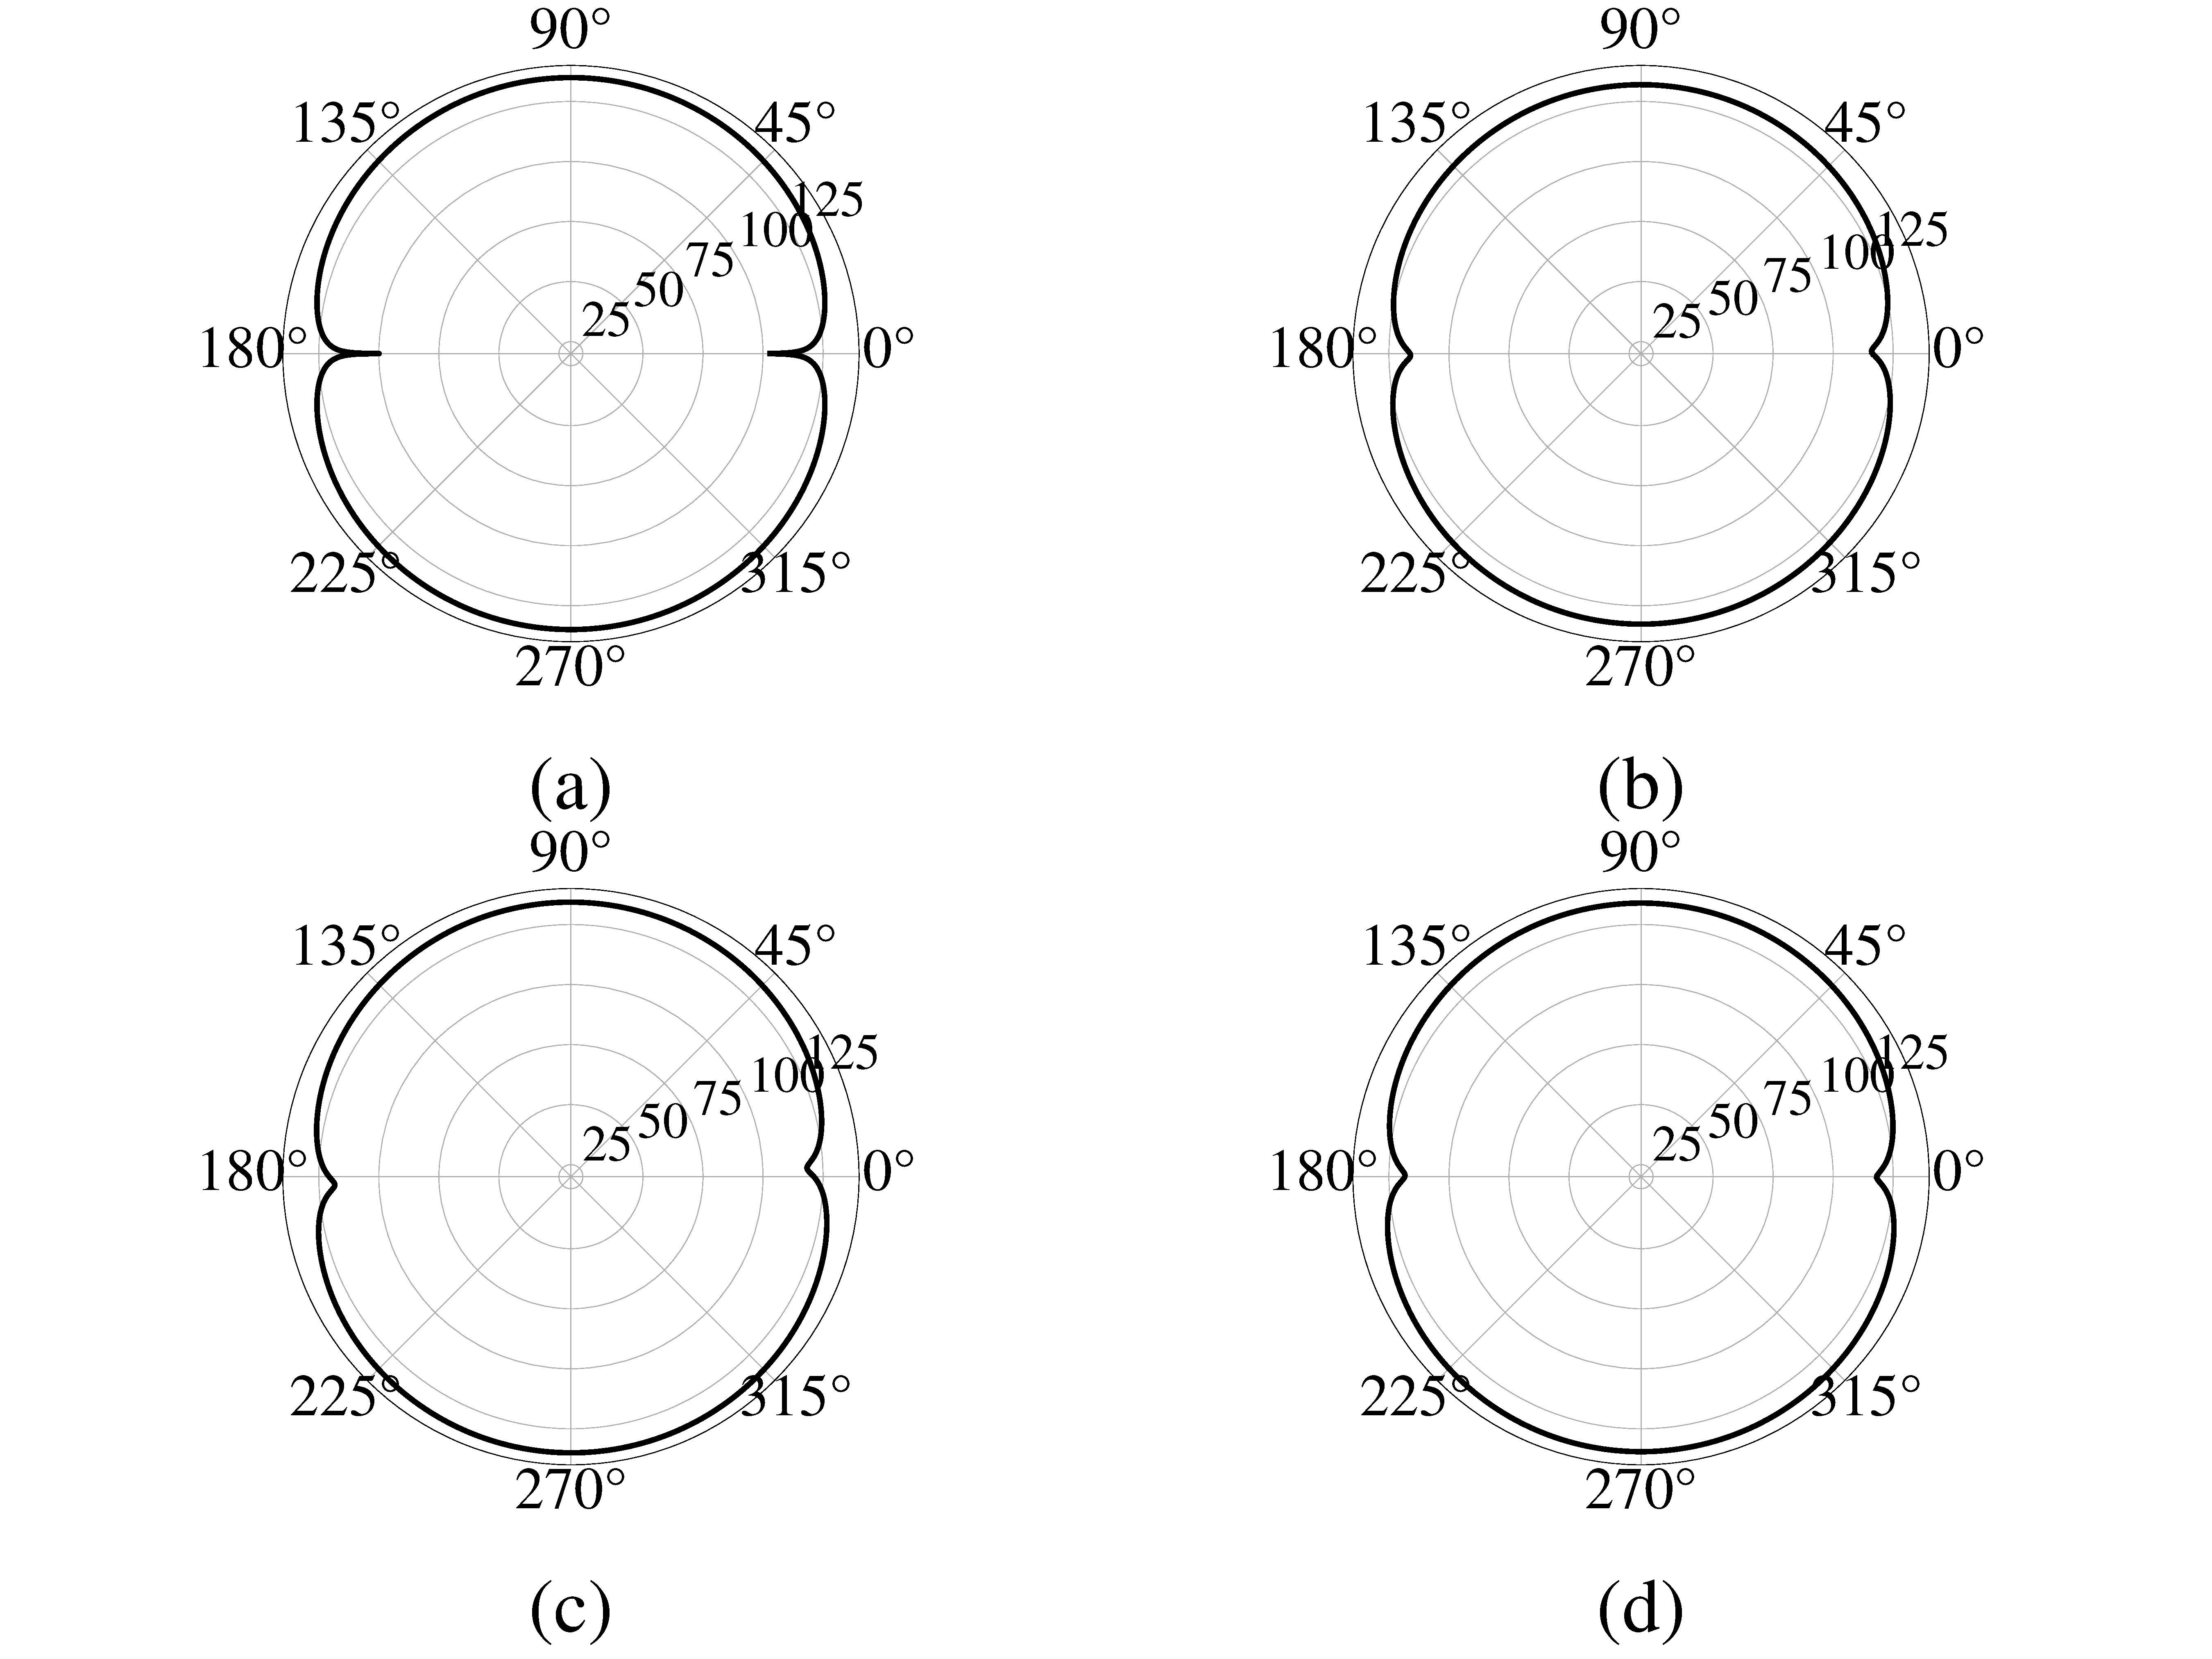
\includegraphics[width=4.9in]{polarplot_sin_theta.eps}}
    \caption{(a):~Azimuthal variation in the exterior pressure field $\Hat{p}_0(\theta,k_z) =\sin(\theta)$. (b), (c) and (d):~Azimuthal variation in the interior pressure field ($r=a$) at 10~Hz, 100~Hz and 1000~Hz, respectively, for $\Hat{p}_0(\theta,k_z) =\sin(\theta)$.}
    \label{polar plot sin theta}
\end{figure}

Fig.~\ref{polar plot sin theta}(a) shows the azimuthal variation in the acoustic pressure (see Eqs.~(\ref{acoustic pressure field inside}) - (\ref{SPL for theta variation}) with $\Hat{p}_f$ being replaced with $\sin(\theta)$) at the outer surface of the elastic tube. Figs.~\ref{polar plot sin theta}(b)~-~\ref{polar plot sin theta}(d) shows the resulting azimuthal variation in the acoustic pressure at the inner surface (r=a) of the elastic tube for (b):~10~Hz, (c)~100~Hz and (d)~1000~Hz. Fig.~\ref{polar plot cos theta} shows similar results for $\Hat{p}_0(\theta,k_z) = \cos(\theta)$. The Figs.~\ref{polar plot sin theta} and \ref{polar plot cos theta}
confirms that the 3D-VA model accurately captures the azimuthal variation (restricted to $n=0$ and $n=1$) in the external pressure excitation.

\begin{figure}[ht]
    \centerline{
    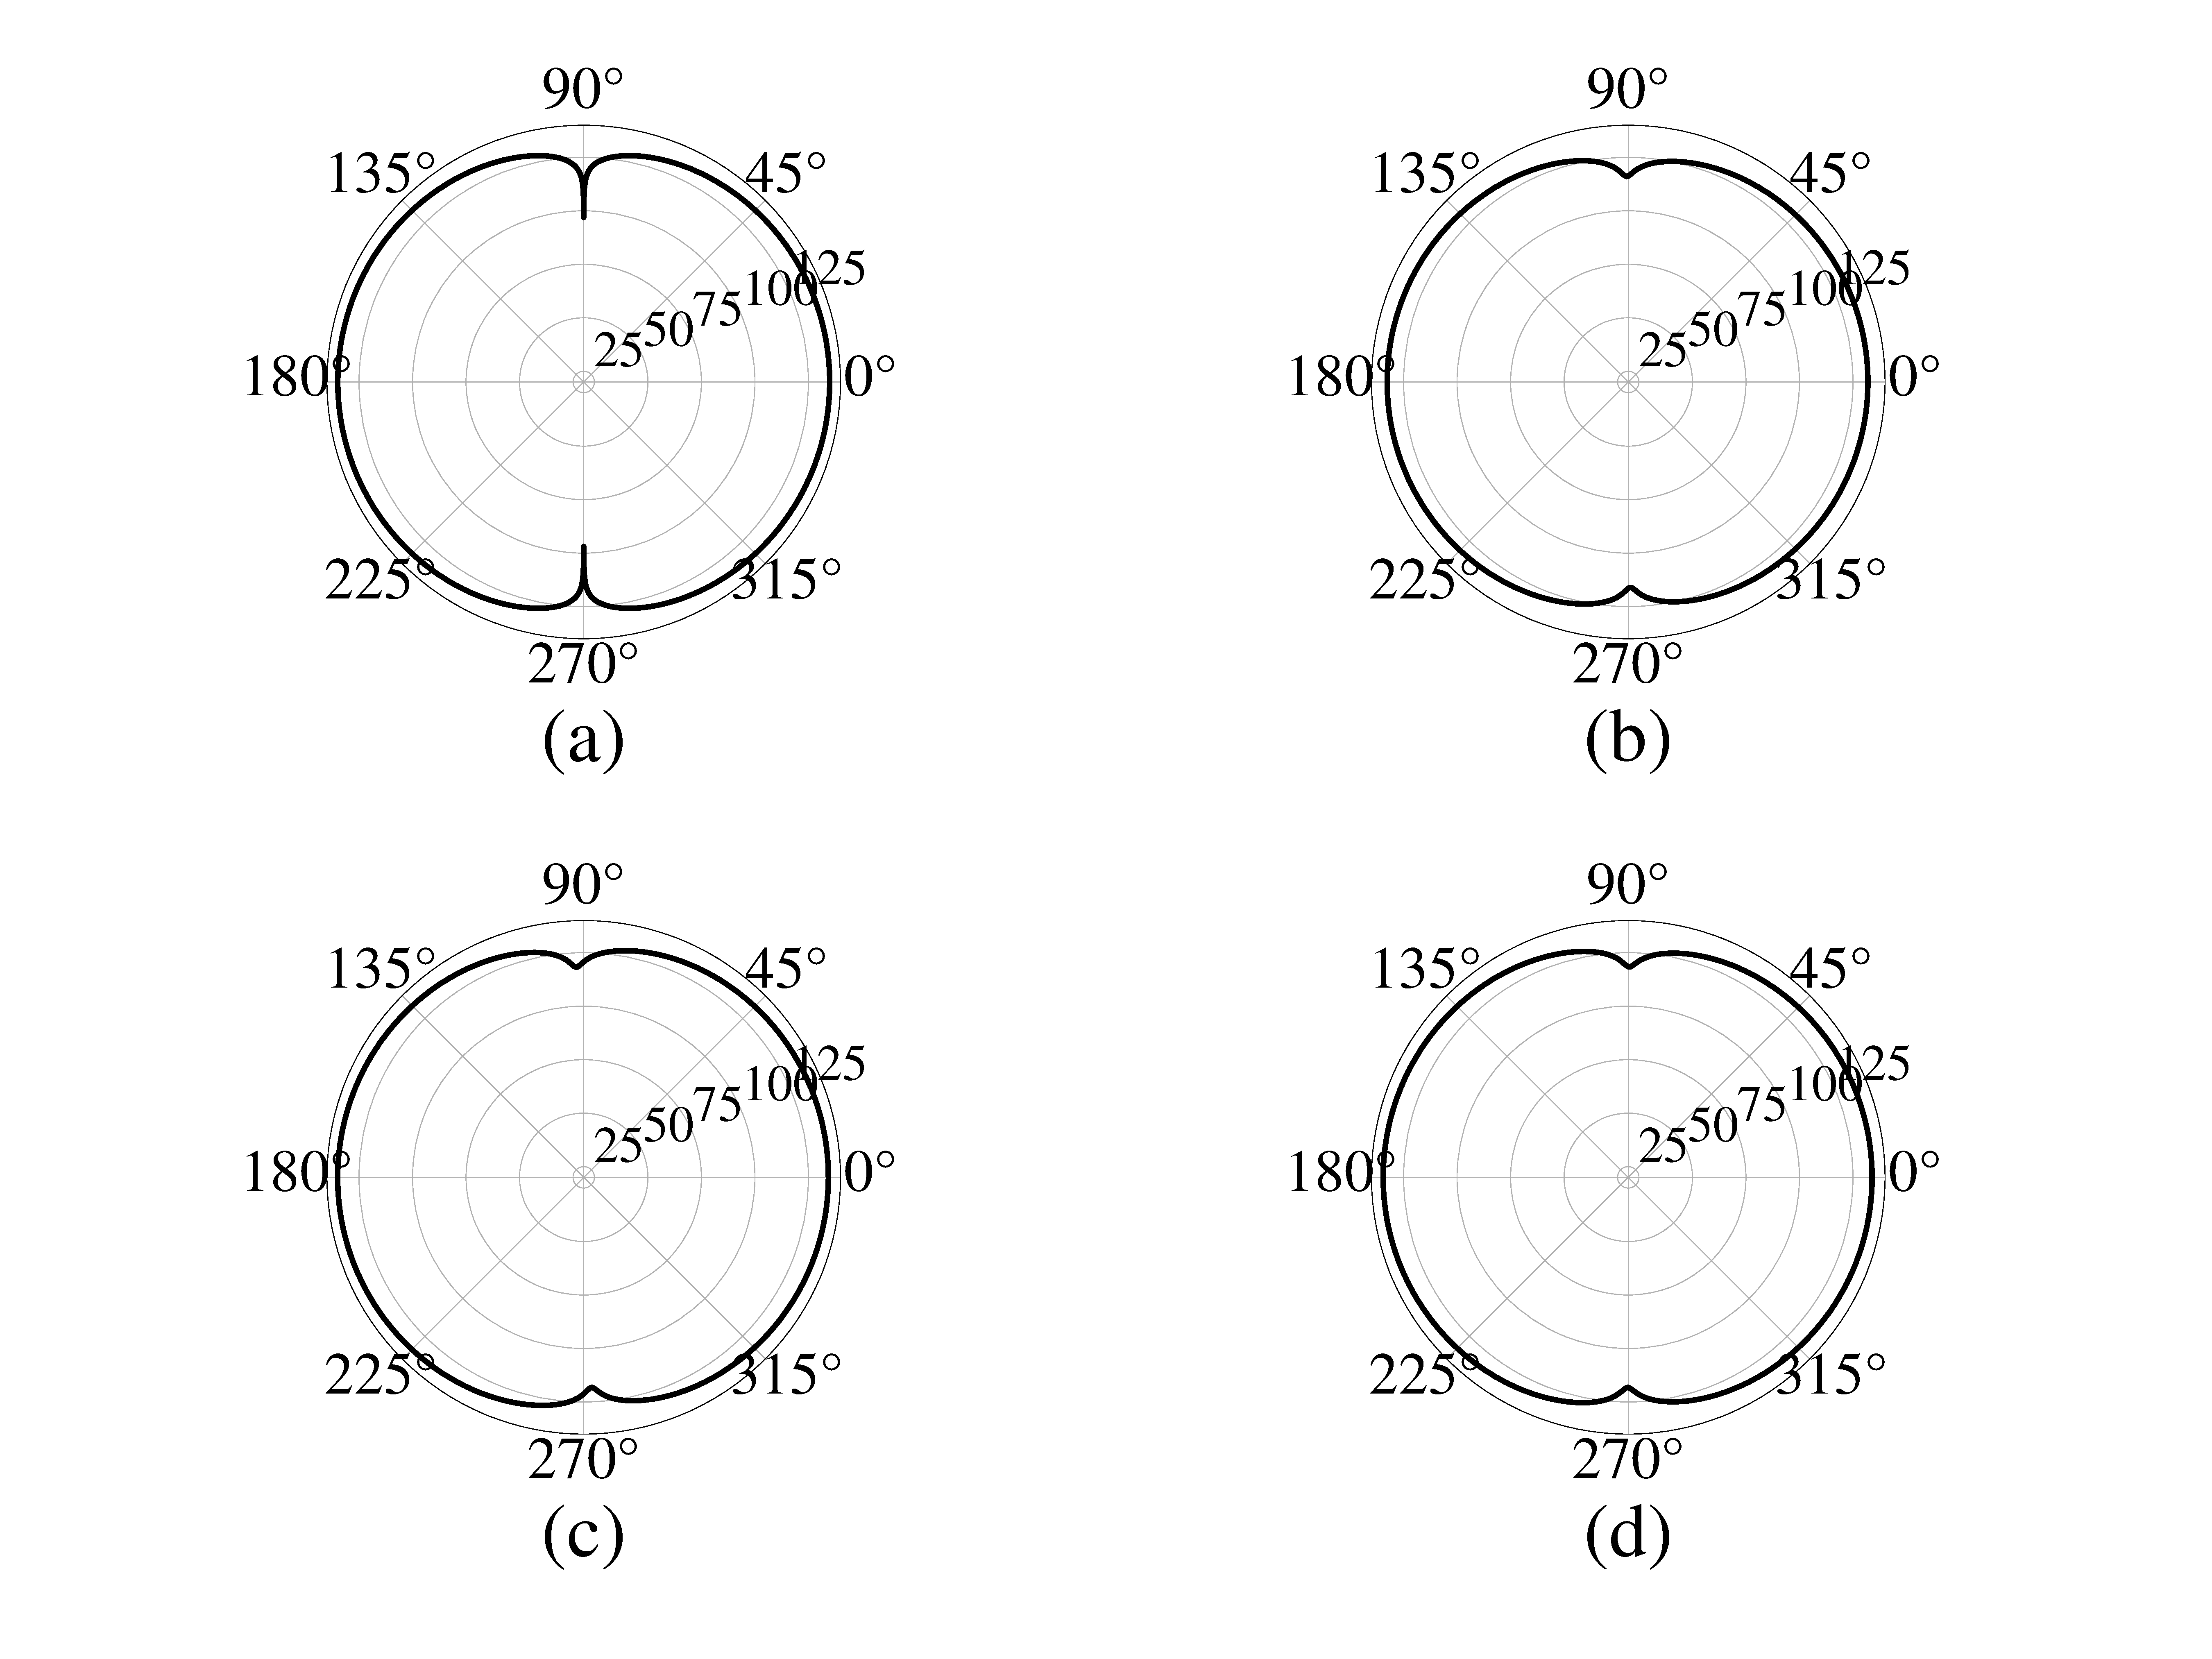
\includegraphics[width=4.9in]{polarplot_cos_theta.eps}}
    \caption{(a):~Azimuthal variation in the exterior pressure field $\Hat{p}_0(\theta,k_z) =\cos(\theta)$. (b), (c) and (d):~Azimuthal variation in the interior pressure field ($r=a$) at 10~Hz, 100~Hz and 1000~Hz, respectively, for $\Hat{p}_0(\theta,k_z) =\cos(\theta)$.}
    \label{polar plot cos theta}
\end{figure}

%%%%%%%%%%%%%%%%%%%%%%%%%%%%%%%%%%%%%%%%%%%%%%%


\begin{figure}[ht]
    \centerline{
    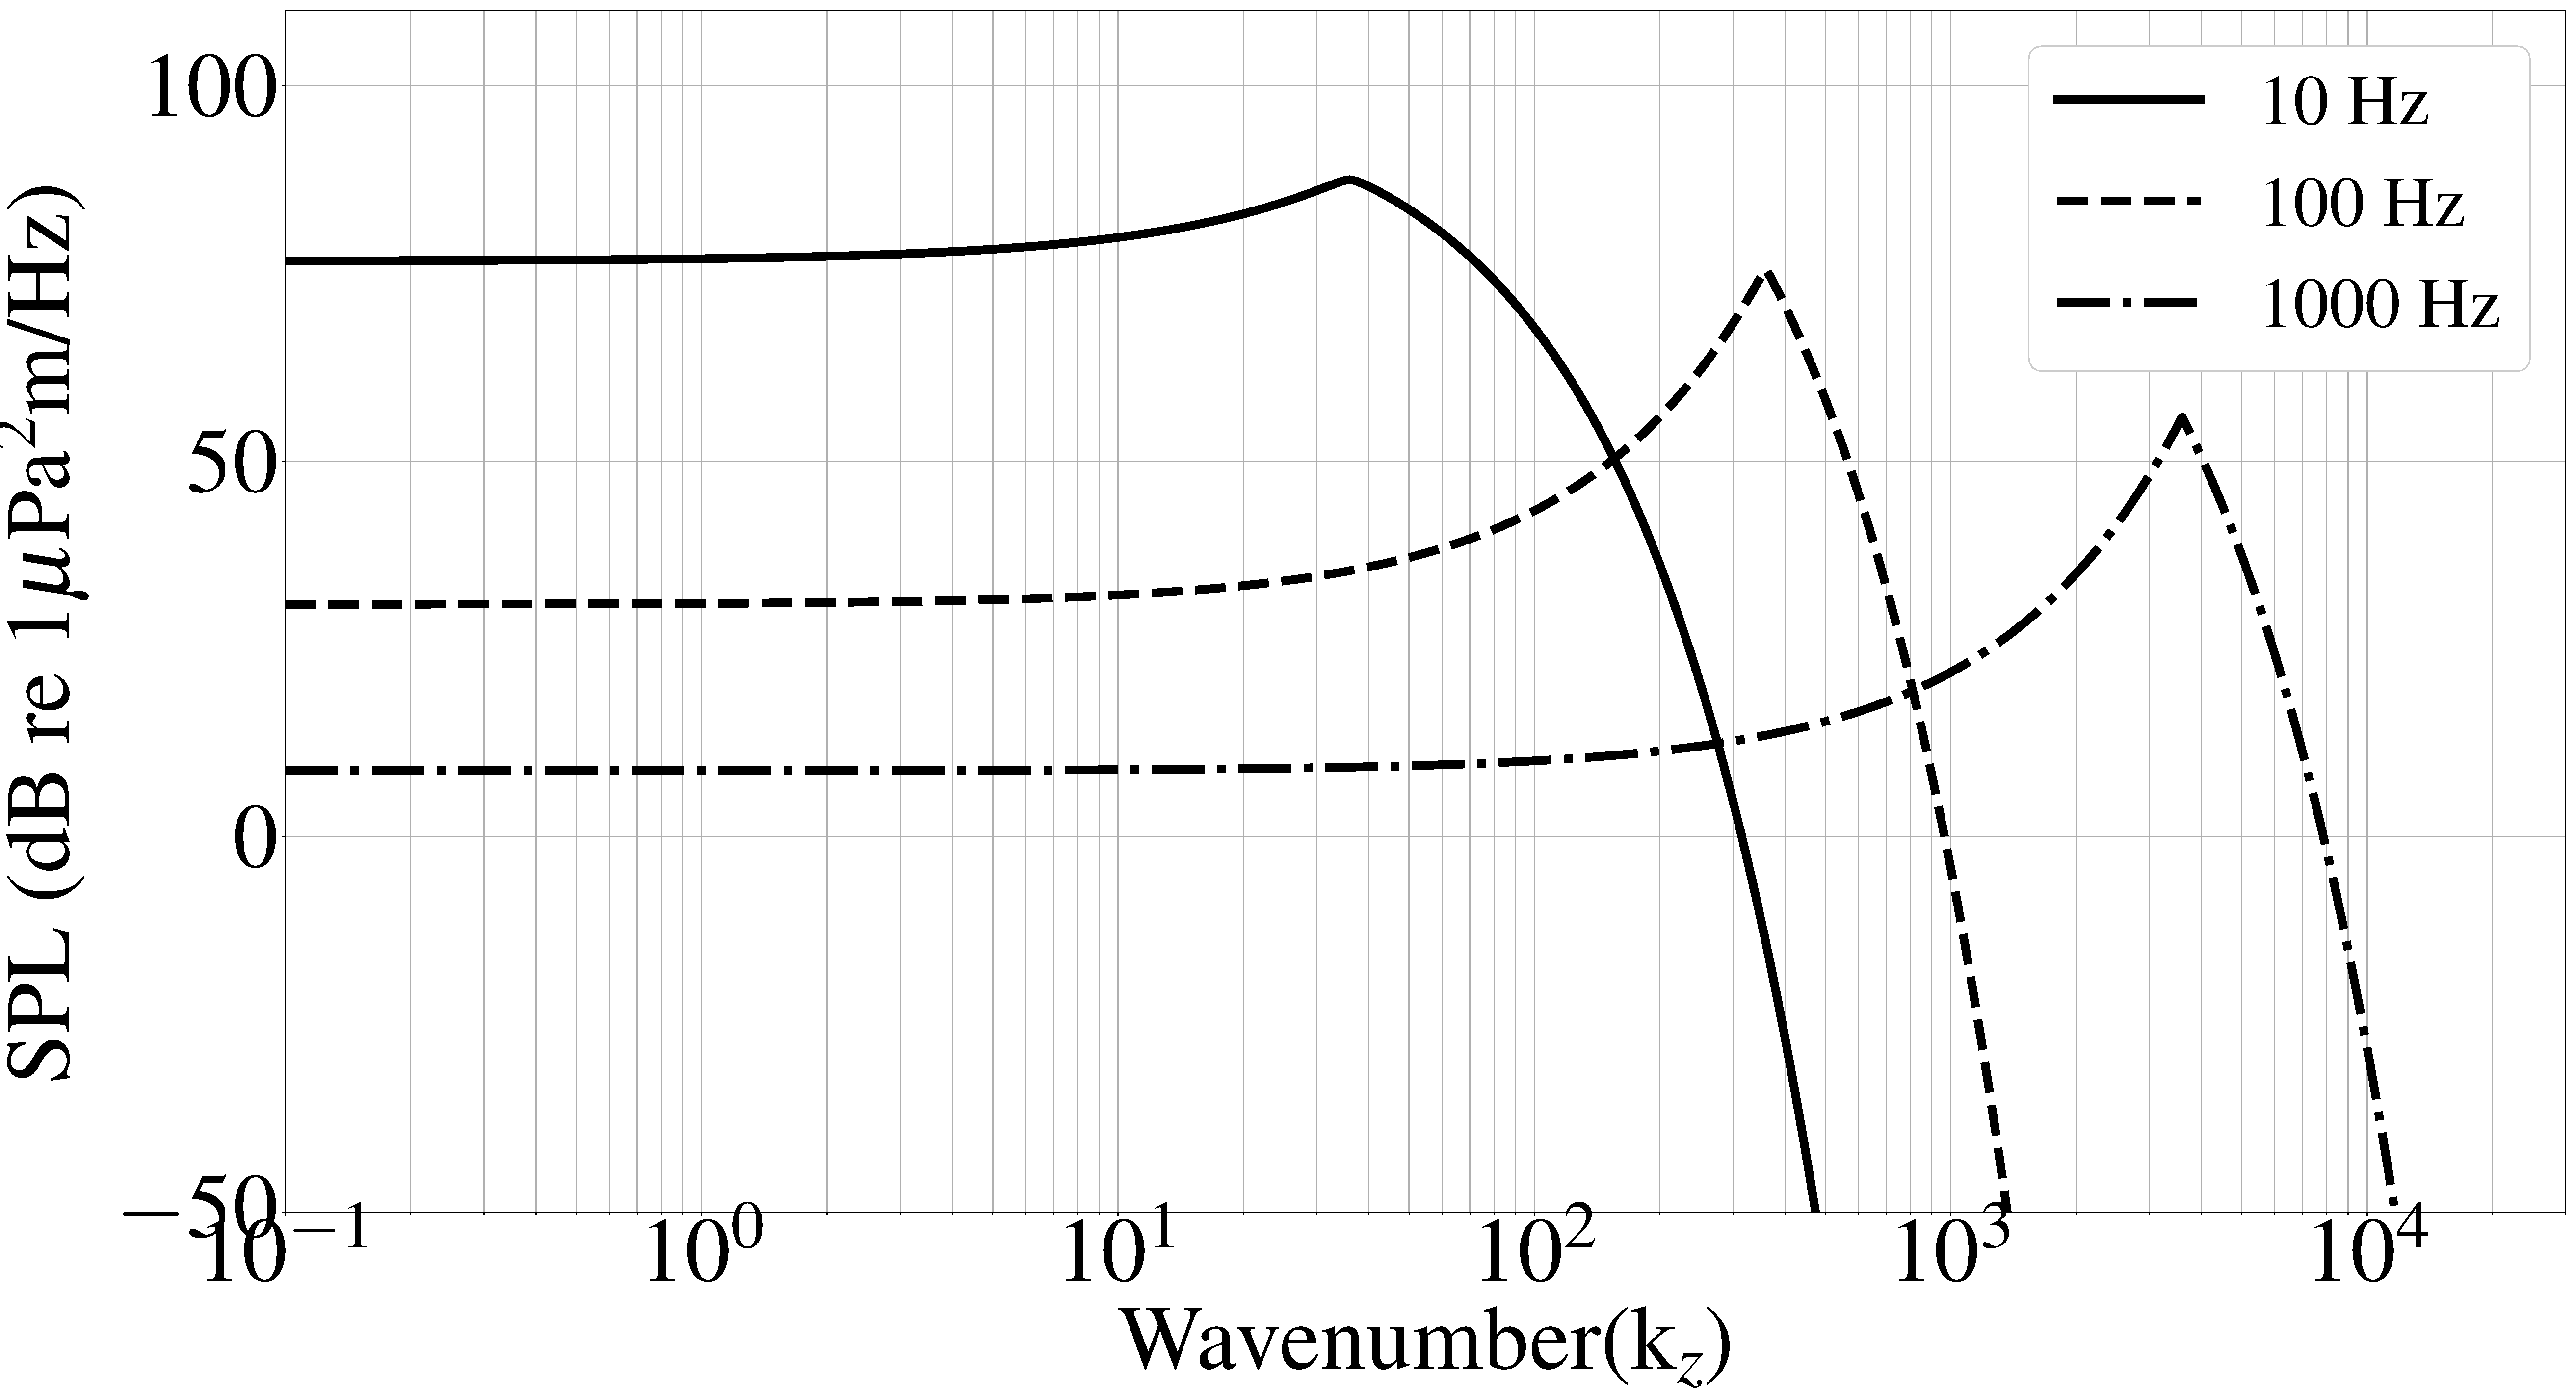
\includegraphics[width=4.3in]{Comparison_of_turbulent_pressure_spectrum_of_Hybrid.eps}}
    \caption{The external turbulent pressure spectrum level computed using the hybrid model~(Eq.~(\ref{hybrid model turbulent pressure})).}
    \label{Hybrid turbulent pressure spectrum}
\end{figure}


\subsection{On-axis flow noise spectrum level for external turbulent pressure excitation}
\label{Interior pressure}
This section presents on-axis flow noise spectrum when the elastic tube is excited by an external turbulent pressure field. The external turbulent pressure field (see Fig.~\ref{Hybrid turbulent pressure spectrum}) is computed using the hybrid model (Eq.~(\ref{hybrid model turbulent pressure})). Further, the 3D-VA model is used to calculate the on-axis flow noise spectrum~(see Eqs.~(\ref{on-axis flow noise spectrum}) and (\ref{SPL flow noise spectrum})). This flow noise spectrum is compared with that computed using the tube transfer function model~\cite{knight1996} (see Fig.~\ref{3d vs approx}) and the axisymmetric model~\cite{jineesh2013} (see Fig.~\ref{3d vs axi}). The elastic tube, inside fluid, and hydrophone array parameters used for computation are listed in Table~\ref{tab:PresentVsJineesh}.
\begin{table}[t]
\caption{The elastic tube, interior fluid and the hydrophone array parameters used for estimation of flow noise inside the cylinder}
\begin{center}
\label{tab:PresentVsJineesh}
\begin{tabular}{l l}
& \\ % put some space after the caption 
 \hline
 \textbf{Property} & \textbf{Values}  \\ 
 \hline
 Tube diameter (m)  & 0.04 \\
% \hline
 Tube thickness (m) & 0.005 \\
% \hline
 Tow speed/Flow velocity (knots) & 5 \\
% \hline
 Number of hydrophones & 50 \\
% \hline
 Length of hydrophone (m) & 0.05 \\
% \hline
 Hydrophone spacing (m) & 0.25 \\
% \hline
 Exterior fluid density (kg/m$^{3}$) & 1000 \\
% \hline
 Interior fluid density (kg/m$^{3}$) & 800 \\
% \hline
 Reference pressure ($\mu$ Pa) & 1  \\ 
\hline
\end{tabular}
\end{center}
\end{table}
It can be seen from Figs.~\ref{3d vs approx} and \ref{3d vs axi} that the on-axis acoustic pressure computed using the 3D-VA model follows the external turbulent pressure excitation given in Fig.~\ref{Hybrid turbulent pressure spectrum} - gradually increasing up to and peaking at the convective wavenumber~($u_c = \omega/k_c$), and decreasing exponentially beyond. Thus, the flow noise inside the tube is dominated by the contribution from wavenumbers less than the convective wavenumber.

\begin{figure}
    \centerline{
    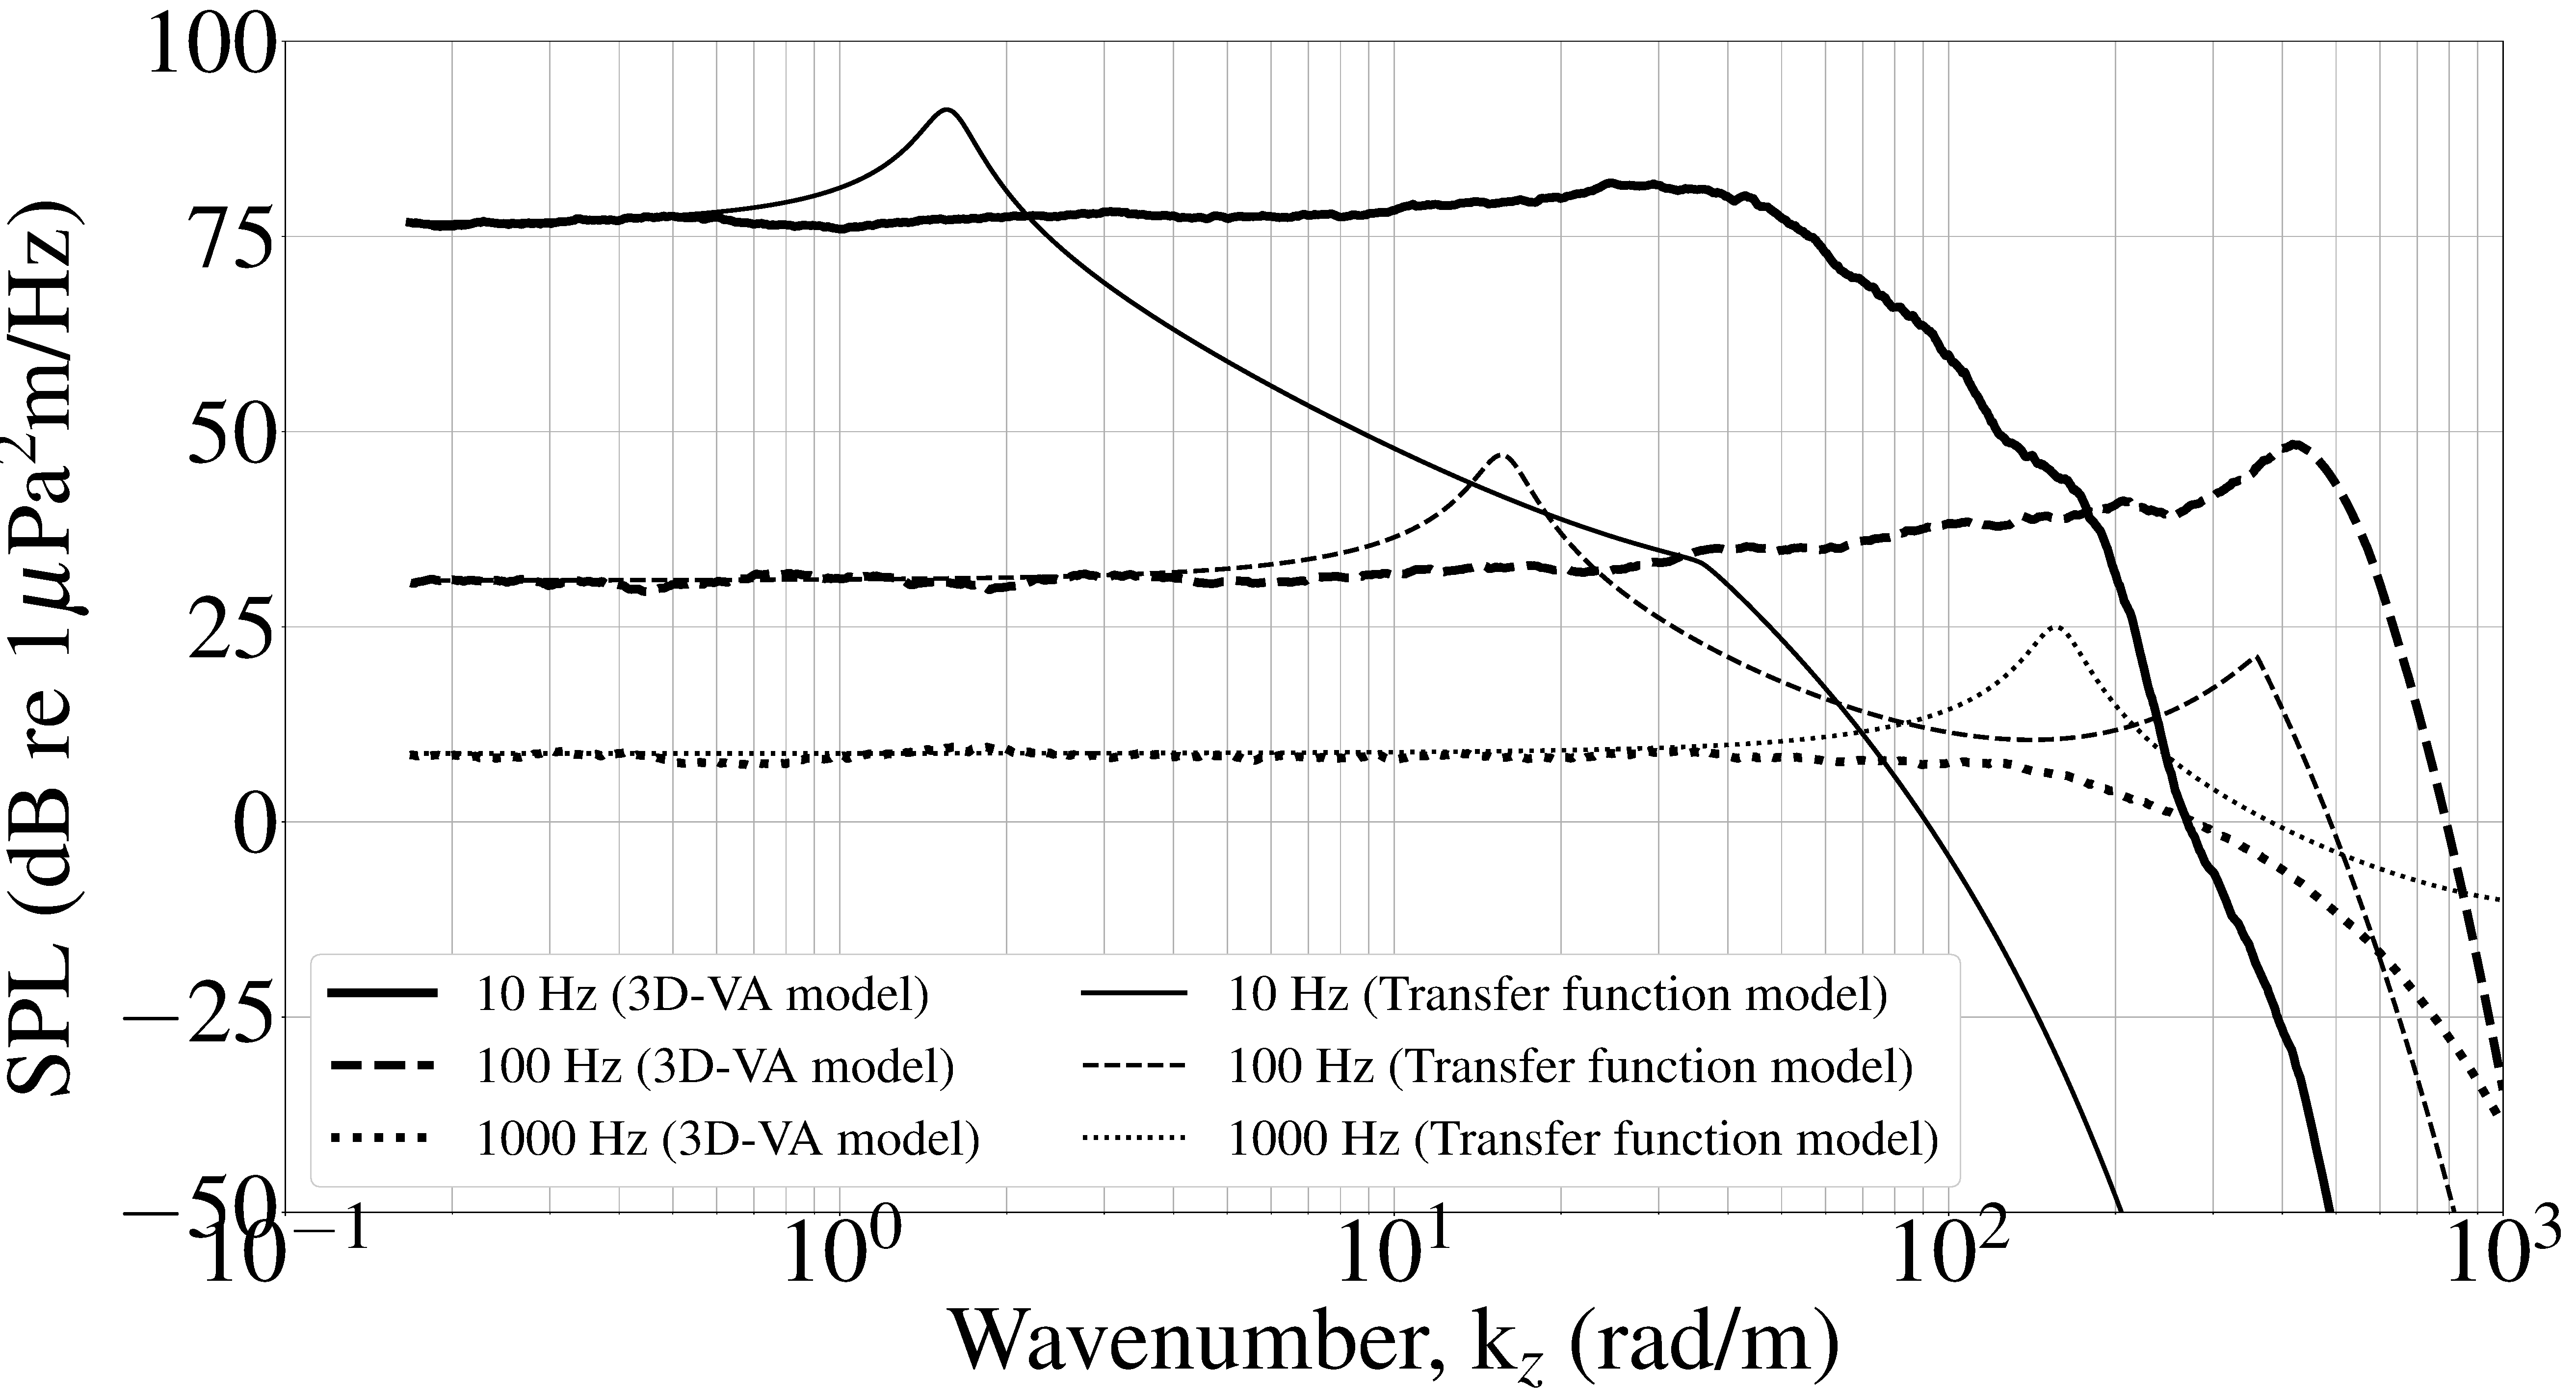
\includegraphics[width=4.3in]{Inside_pressure_comparison_3d_and_approx.eps}}
    \caption{Comparison of on-axis flow noise spectrum level due to a turbulent pressure excitation computed using the 3D-VA model and the tube transfer function model~\cite{knight1996}.} 
    \label{3d vs approx}
\end{figure}
\begin{figure}
    \centerline{
    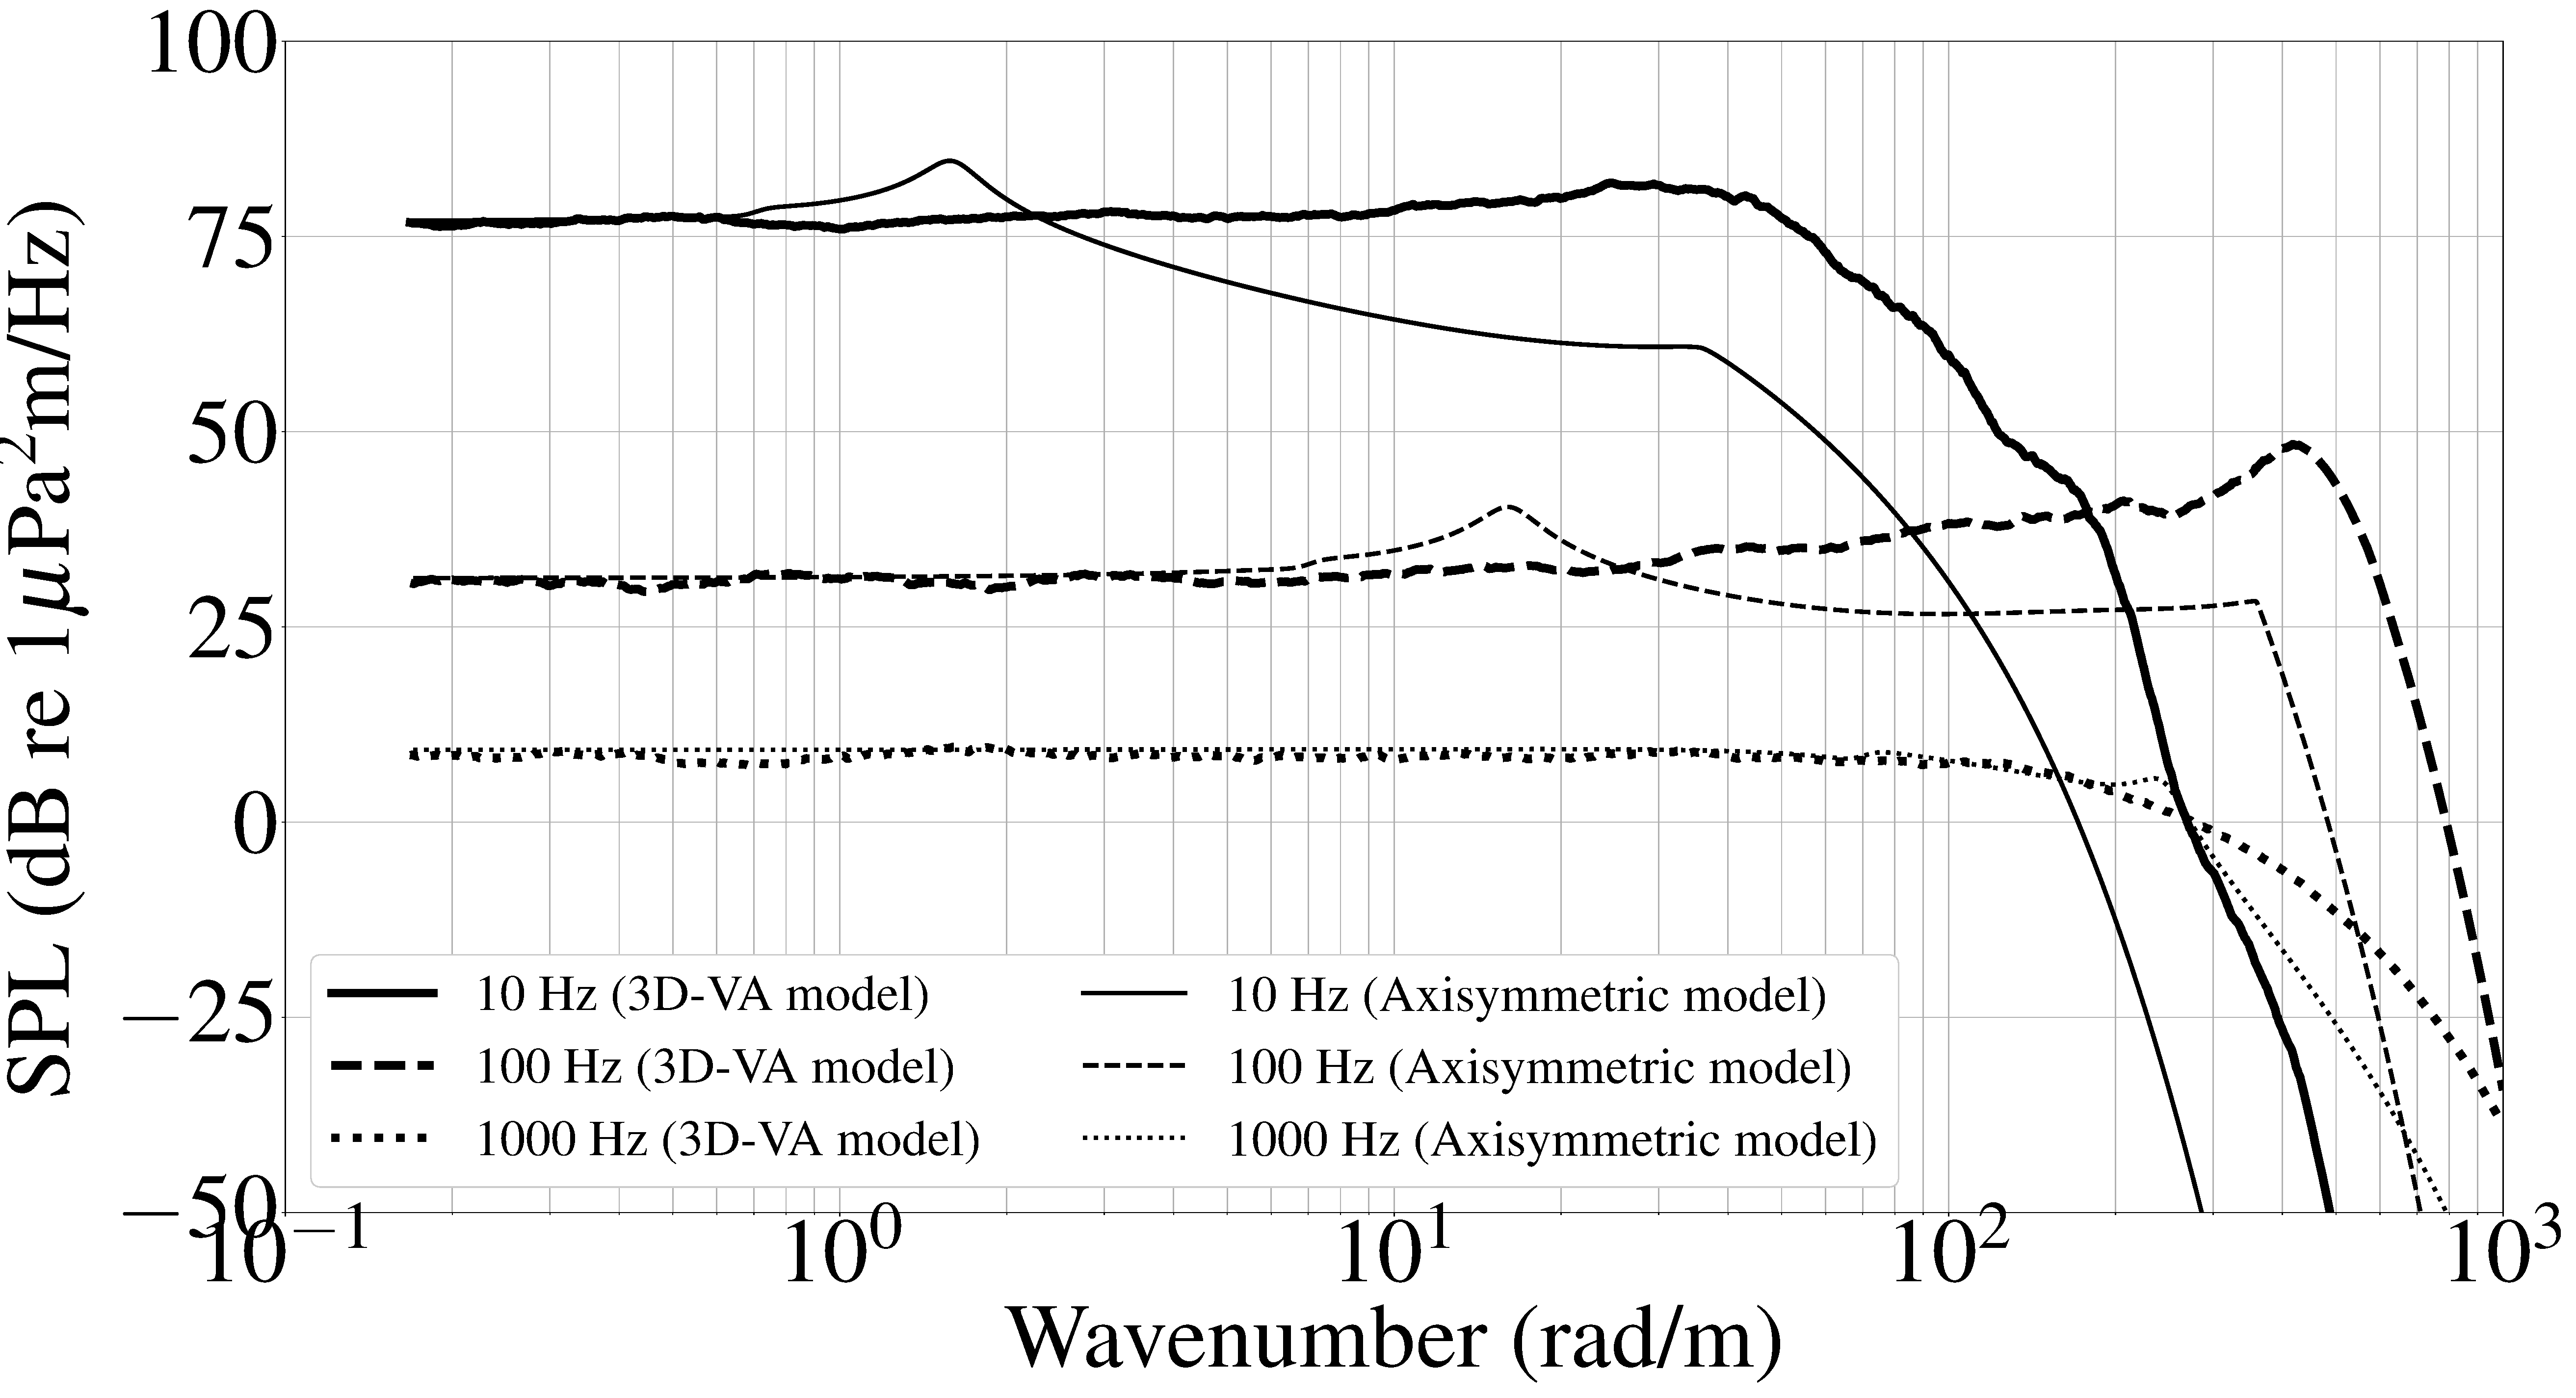
\includegraphics[width=4.3in]{Inside_pressure_comparison_3d_and_axi.eps}}
    \caption{Comparison of on-axis flow noise spectrum level due to a turbulent pressure excitation computed using the 3D-VA model and the axisymmetric model~\cite{jineesh2013}.}
    \label{3d vs axi}
\end{figure}

In the tube transfer function model (Fig.~\ref{3d vs approx}) and the axisymmetric model (Fig.~\ref{3d vs axi}) predictions, the peak occurs at a lower wavenumber than the convective wavenumber. For example, at 10~Hz, the peak occurs at $1.58$~rad/m in the tube transfer function model and at $1.56$~rad/m in the axisymmetric model. Note that the convective wavenumber at 10~Hz for 5~knots is $k_c = 35.93$~rad/m. This smaller wavenumber where the first peak occurs in the transfer function and the axisymmetric models corresponds to the breathing mode wavenumber, $k_b$, of the elastic tube given by~\cite{knight1996}
\begin{equation}\label{breathing wavenumber}
k_b^2 = 2\rho_0\omega^2R/Et.
\end{equation}
In Eq.~(\ref{breathing wavenumber}), $\rho_0$ is the density of the inside fluid, $R$ is the outer radius of the elastic tube, $E$ is the Young's modulus of the tube and $t$ is the thickness of the tube. The tube transfer function model and the axisymmetric model consider only the breathing mode~($n=0$) variations while modeling the fluid-filled elastic tube. The present 3D-VA model considers both $n=0$~(breathing) and $n=1$~(first order) variations in the solid and fluid displacement fields. The absence of peaks at the breathing wavenumber in the present 3D-VA model indeed demonstrates a cumulative effect of including both $n=0$ and $n=1$ order terms in the fully-coupled vibroacoustic formulation. The same is the reason for the difference in the flow noise spectrum between the 3D-VA model and the other models beyond the breathing wavenumber.


%%%%%%%%%%%%%%%%%%%%%%%%%%%%%%%%%%%%%%%%%%%%%%%%

\subsection{On-axis flow noise for external turbulent pressure excitation}
\label{on-axis flow noise}

This section presents the flow noise as heard by the hydrophones placed inside the fluid-filled elastic tube. The flow noise is computed using Eqs.~(\ref{on axis flow noise equation}) and (\ref{spl on-axis flow noise}). Note that flow noise at a given frequency can be obtained by integrating the corresponding flow noise spectrum~(Figs.~\ref{3d vs approx} and \ref{3d vs axi}) over the wavenumber. Fig.~\ref{3d vs knight vs jineesh} shows the variation in flow noise with frequency, computed using the 3D-VA model. It also depicts the flow noise predicted by the tube transfer function~\cite{knight1996} and the axisymmetric~\cite{jineesh2013} models. Note that in all cases, the external turbulent pressure excitation is given by Eq.~(\ref{hybrid model turbulent pressure})~(the hybrid model). The elastic tube, interior fluid and hydrophone parameters are given in Table~\ref{tab:PresentVsJineesh}.
\begin{figure}
    \centerline{
    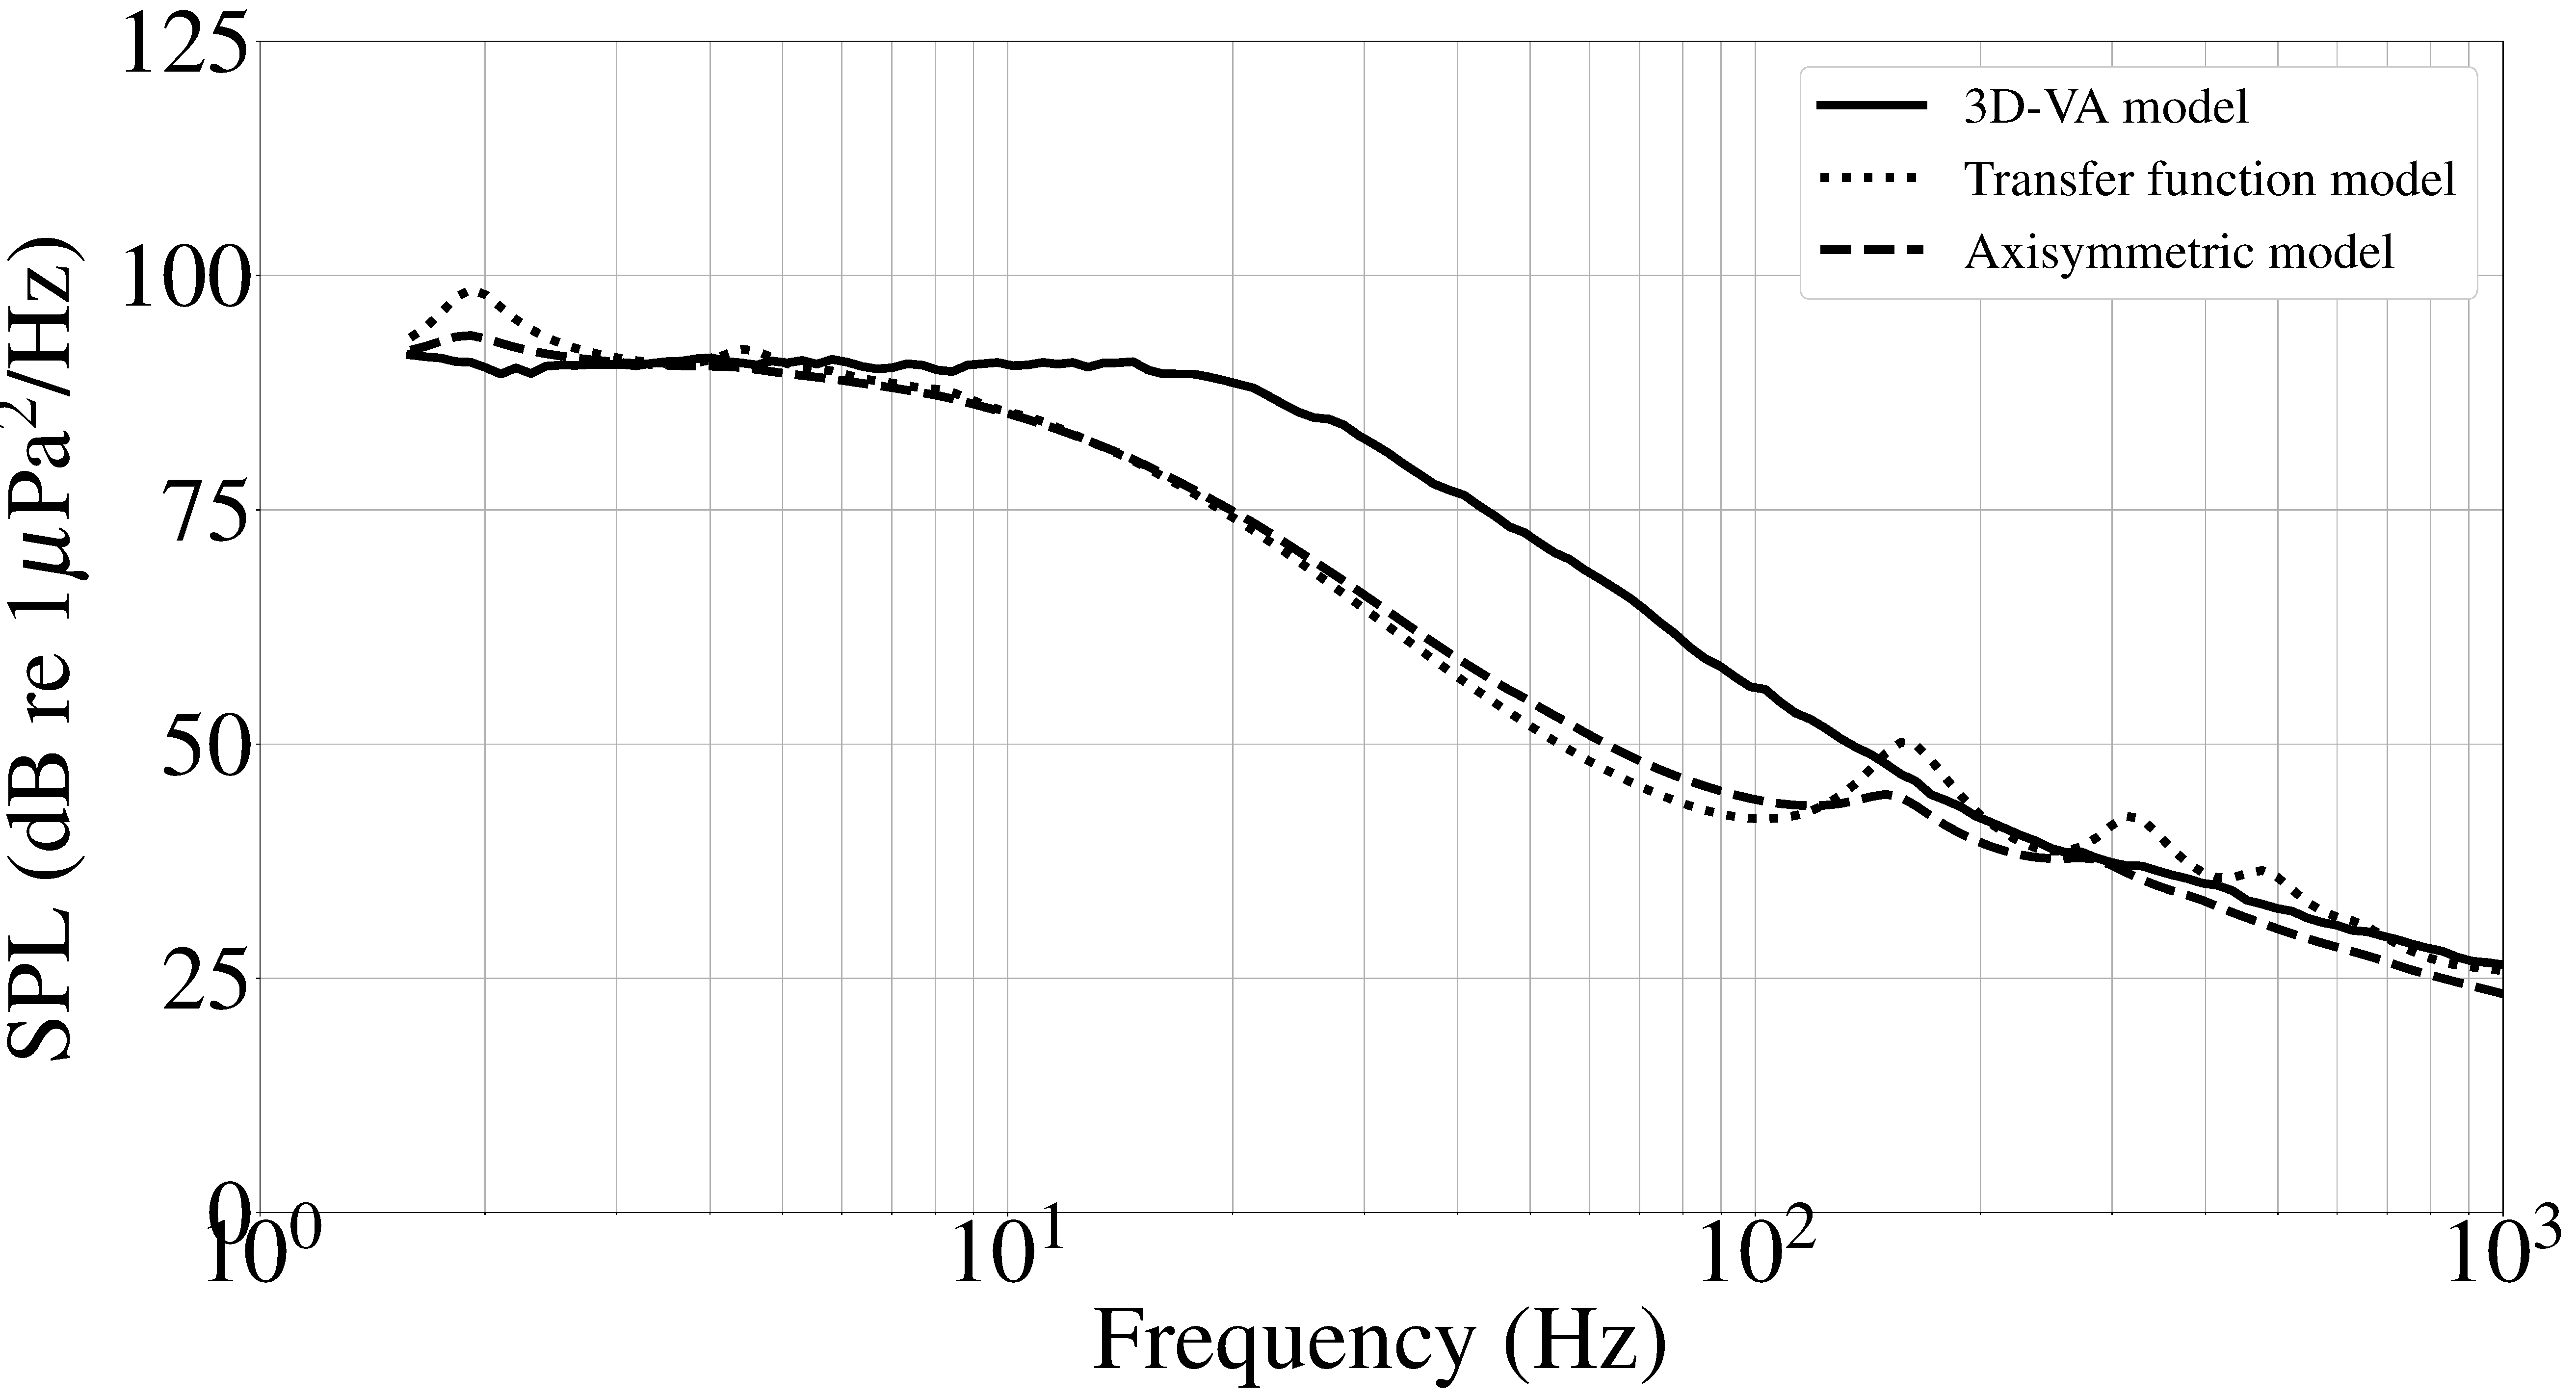
\includegraphics[width=4.3in]{Flow_noise_comparison_3D_vs_Knight_Jineesh.eps}}
    \caption{The on-axis flow noise due to the turbulent pressure excitation computed using the 3D-VA model, the tube transfer function model~\cite{knight1996} and the axisymmetric model~\cite{jineesh2013}.} 
    \label{3d vs knight vs jineesh}
\end{figure}
 It can be seen from Fig.~\ref{3d vs knight vs jineesh} that the flow noise decreases with frequency. This decrease is attributed to the reduction in the external turbulent pressure excitation with frequency as shown in Fig.~\ref{Hybrid turbulent pressure spectrum}. As mentioned earlier, the 3D-VA model considers both $n=0$~(breathing) and $n=1$ variation in the acoustic pressure field. This results in a better flow noise prediction than the transfer function and axisymmetric models, where only the $n=0$ or the breathing wavenumber is considered. The transfer function and the axisymmetric models underpredict the flow noise in the mid frequency range (10~Hz - 200~Hz). It is evident from Figs.~\ref{3d vs approx} and~\ref{3d vs axi} that the difference between the 3D-VA and other models is not significant as the frequency increases. For that reason, the flow noise predictions (Fig.~\ref{3d vs knight vs jineesh}) by the three models are quite close to each other at high frequencies (beyond $\sim$ 200~Hz).

%%%%%%%%%%%%%%%%%%%%%%%%%%%%%%%%%%%%%%%%%%%%%%%%%%

\subsection{On-axis flow noise for different tube diameters and tow speeds}
\label{parametric study}

In this section, the on-axis flow noise~(Eqs.~(\ref{on axis flow noise equation}) and (\ref{spl on-axis flow noise})) is computed for different elastic tube diameters at different tow speeds. Fig.~\ref{flow noise diff dia 3d} shows the comparison of on-axis flow noise estimated for different elastic tube diameters at 5~knots and  Fig.~\ref{flow noise diff speed 3d} shows the variation in the flow noise for a tube of 40~mm diameter at different tow speeds. The variation in flow noise is attributed to the changes in external turbulent pressure excitation with tube diameters and tow speeds, as shown in Fig.~\ref{non dimensional plot of hybrid model}~(the non-dimensional plot). It was shown in Fig.~\ref{non dimensional plot of hybrid model} that an increase in diameter or a decrease in tow speed results in a reduction in the non-dimensional power spectral density. This leads to a decrease in on-axis flow noise inside the fluid-filled elastic tube with increasing tube diameter~(Fig.~\ref{flow noise diff dia 3d}) or decreasing tow speeds~(Fig.~\ref{flow noise diff speed 3d}).

\begin{figure}
    \centerline{
    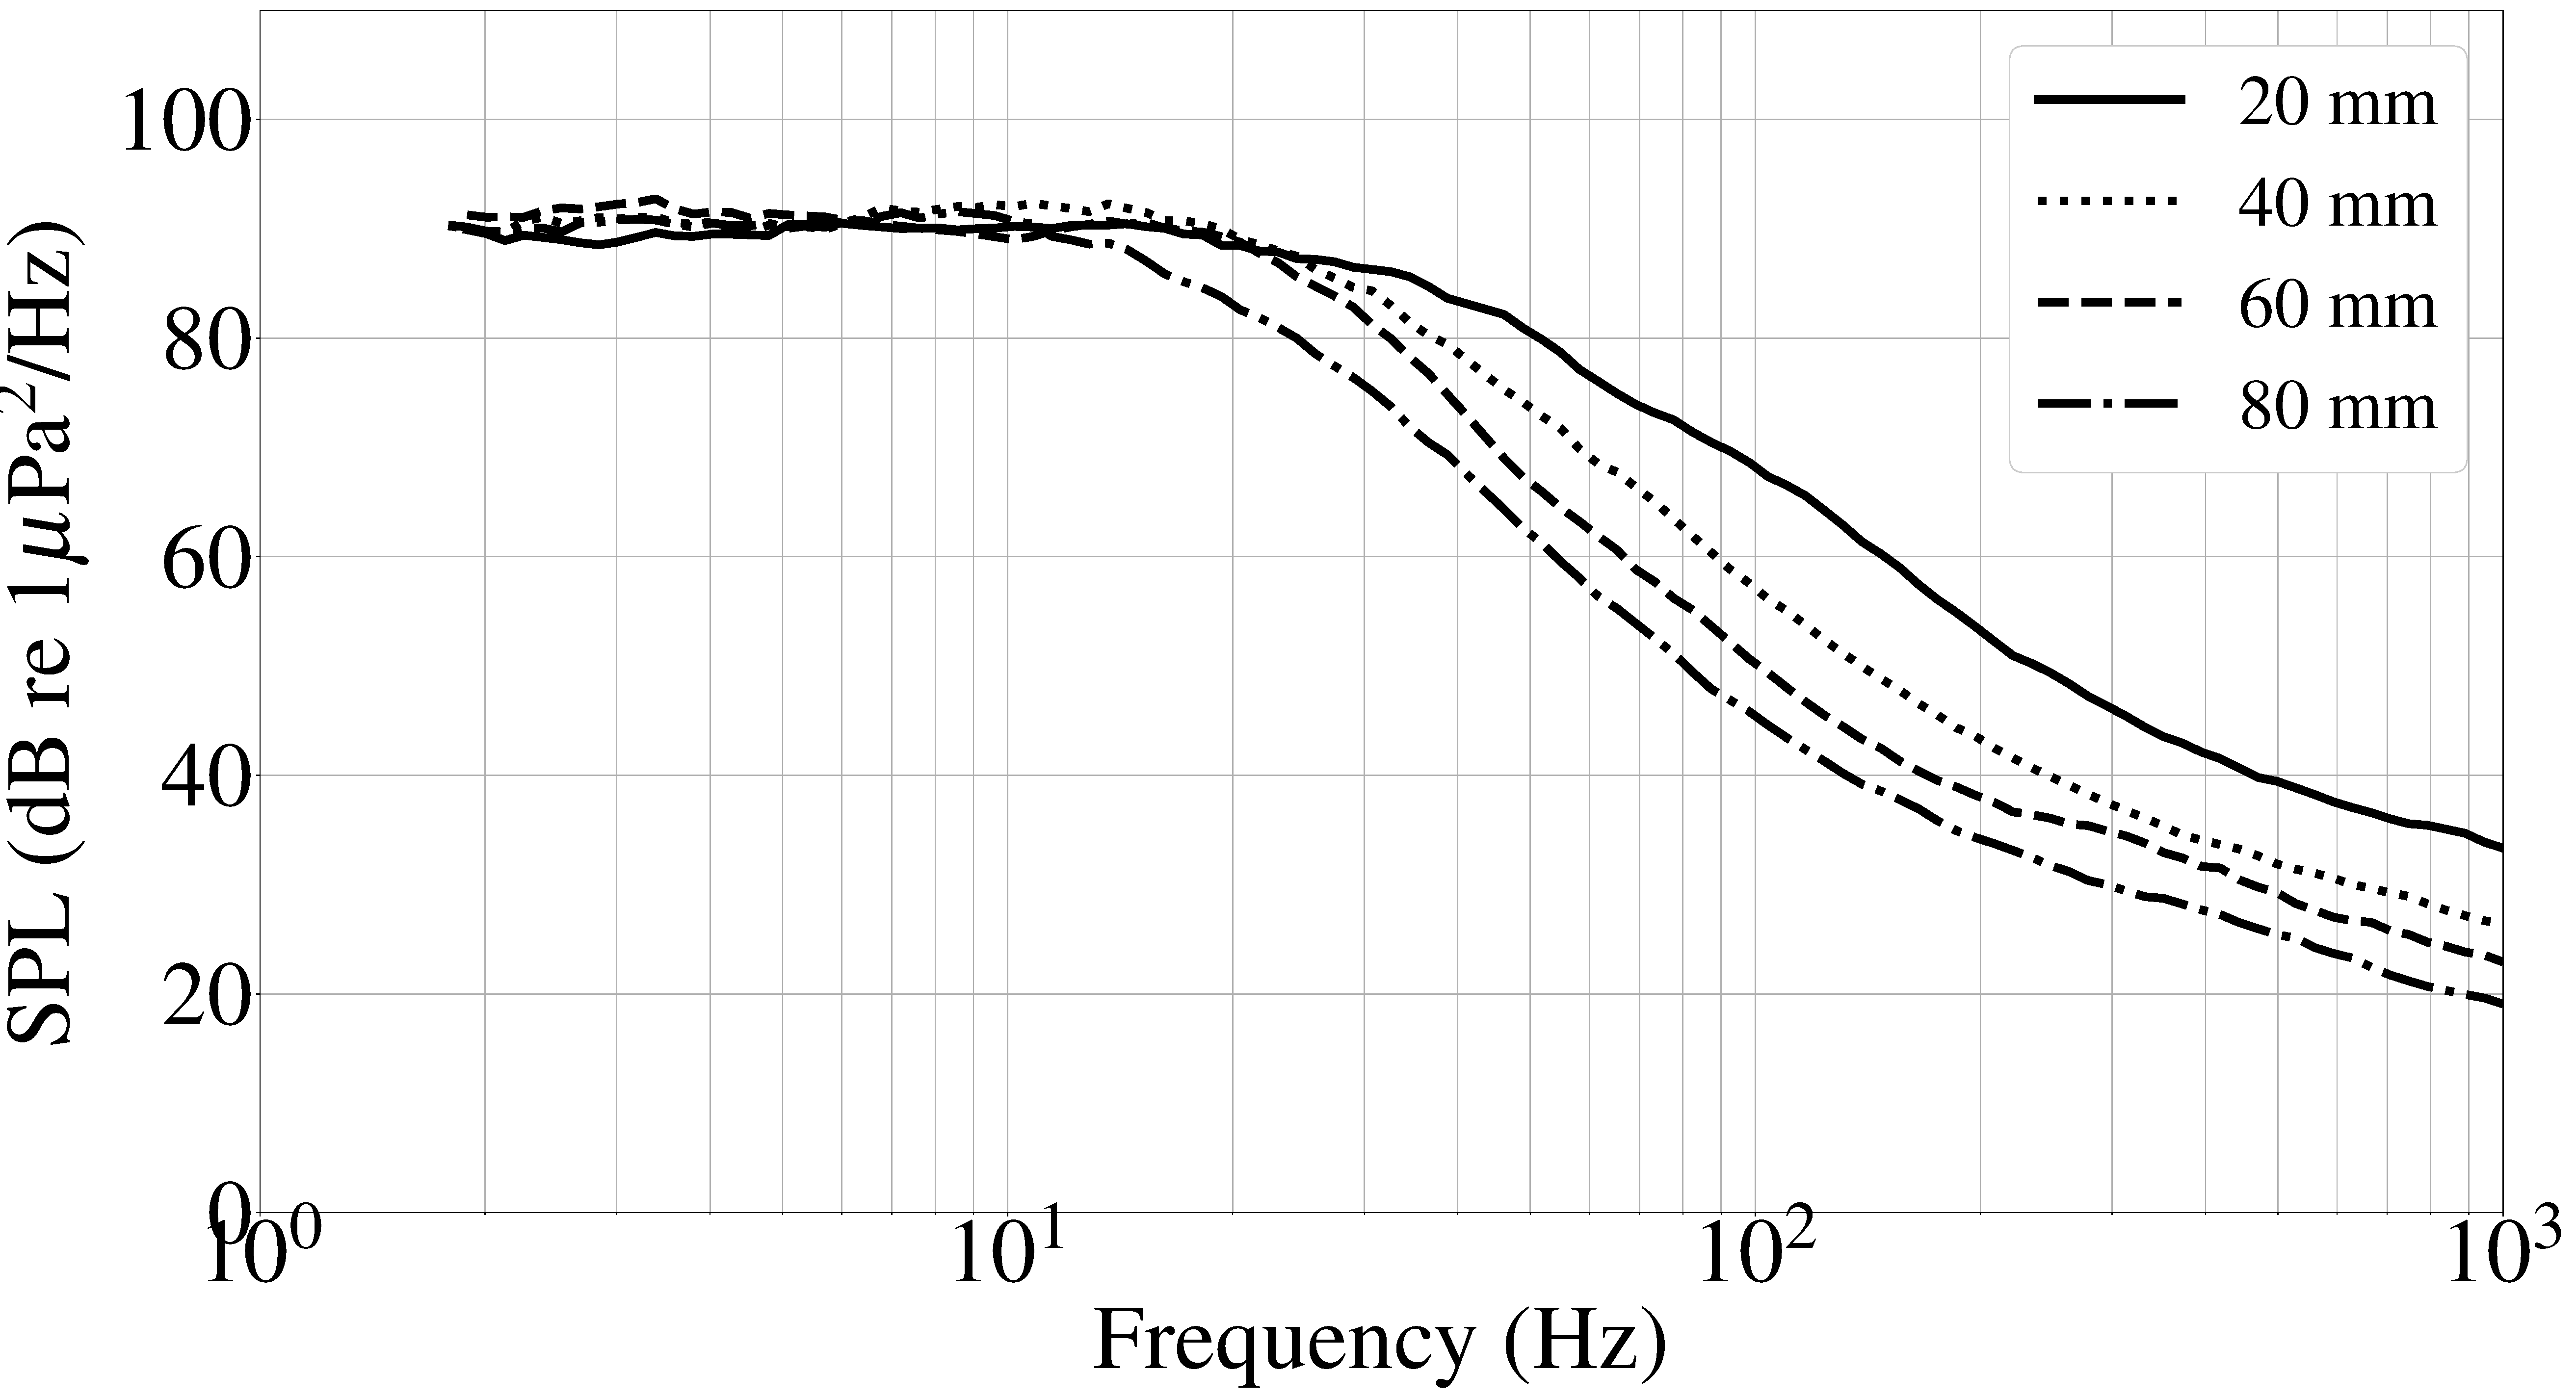
\includegraphics[width=4.3in]{Comparison_of_flow_noise_3D_different_dia.eps}}
    \caption{Comparison of on-axis flow noise estimated using 3D-VA model, due to a turbulent pressure excitation at 5~knots over an elastic tube for different diameters.}
    \label{flow noise diff dia 3d}
\end{figure}
\begin{figure}
    \centerline{
    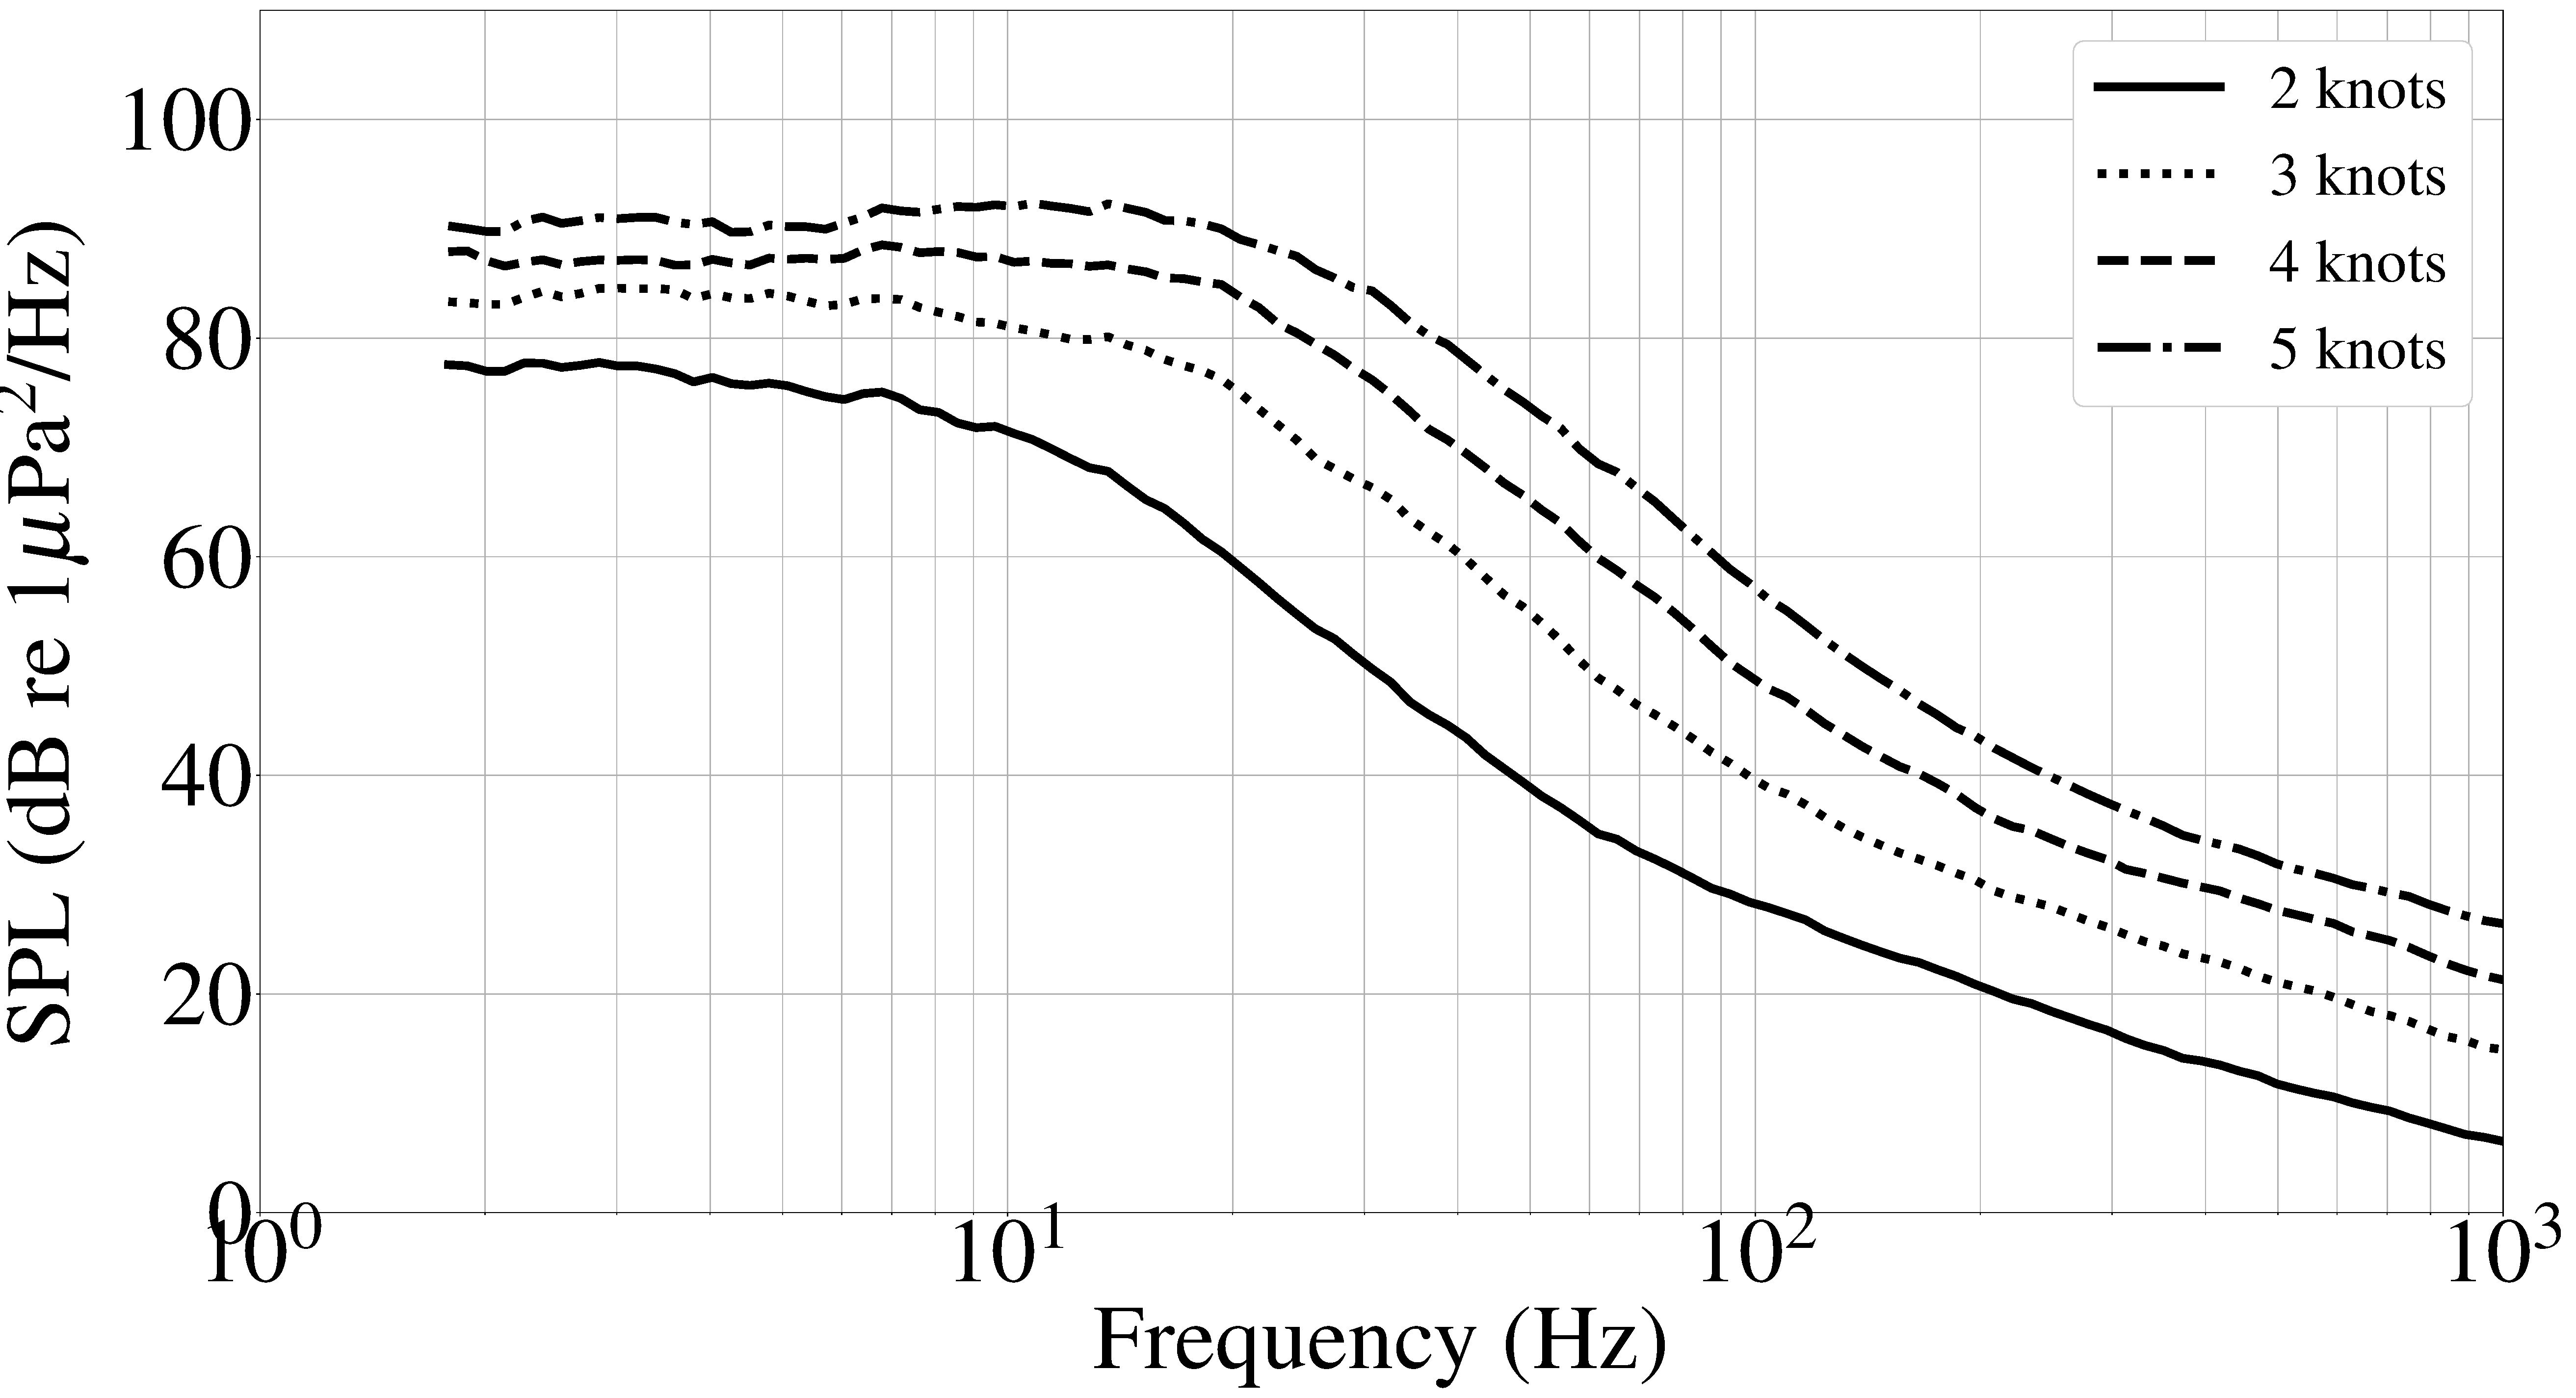
\includegraphics[width=4.3in]{Comparison_of_flow_noise_3D_Different_speed.eps}}
    \caption{Comparison of on-axis flow noise estimated using 3D-VA model, due to a turbulent pressure excitation over an elastic tube of 40~mm diameter at different tow speeds.}
    \label{flow noise diff speed 3d}
\end{figure}


%%%%%%%%%%%%%%%%%%%%%%%%%%%%%%%%%%%%%%%%%%%%%%%%

%%%%%%%%%%%%%%%%%%%%%%%%%%%%%%%%%%%%%%%%%%%%%%%%%%%%%%%%%%%%%%%%%%%%%
%%%%%%%%%%%%%%%%%%%%%%%%%%%%%%%%%%%%%%%%%%%%%%%%%%%%%%%%%%%%%%%%%%%%%%
\section{Conclusions}
A new semi-empirical (hybrid) model is developed for estimating the wavenumber-frequency spectrum of turbulent pressure for an axial flow past a solid cylinder. The hybrid model is derived using insights from different turbulent pressure semi-empirical models (Chase~\cite{Chase1981} and Frendi \textit{et al}.~\cite{frendi2020}) and the experimental results of Unnikrishnan \textit{et al}.~\cite{Unni2011}. The hybrid model predictions are found to be superior to the existing semi-empirical models and compares reasonably well with available experimental results. 


A fully-coupled three-dimensional vibroacoustic model~(3D-VA model) is developed for computing the pressure field inside the fluid-filled elastic tube due to external turbulent pressure excitations. In this 3D-VA model, the structure (elastic tube) is modeled using the Navier-Lame equilibrium equations, and the fluid inside the tube is modeled using the acoustic wave equation. The 3D-VA model is first tested for an exterior harmonic pressure excitation having a known azimuthal variation. The interior pressure field is found to follow the same azimuthal variation as that of the external excitation.

Next, the 3D-VA model is used in conjunction with the hybrid model of the turbulent pressure spectrum to find the on-axis flow noise. The results are then compared with the on-axis flow noise estimated using an existing transfer function model~\cite{knight1996} and an axisymmetric vibroacoustic model. The transfer function and the axisymmetric models consider only the breathing mode~($n=0$) of the elastic tube, but the 3D-VA model considers both $n=0$~(breathing) and $n=1$~(first order) variations in modeling the elastic tube and the fluid inside the tube. Consequently, it is observed that the two other models underpredict the flow noise compared to the 3D-VA model.

The on-axis flow noise is then estimated for different elastic tube diameters and tow speeds. At low frequencies, an increase in the tube diameter causes negligible variation in flow noise, but at higher frequencies, the flow noise decreases with increase in the tube diameter. When the tow speed is increased, the flow noise is found to increase at all frequencies.

%%%%%%%%%%%%%%%%%%%%%%%%%%%%%%%%%%%%%%%%%%%%%%



%%%%%%%%%%%%%%%%%%%%%%%%%%%%%%%%%%%%%%%%%%%%%%%%%%%%%%%%%%%%%%%%%%%%%%
\begin{acknowledgment}
This research was supported by the Defence Research and Development Organisation, India. The authors express their sincere gratitude to Dr.~Ganesh Natarajan and Dr.~Pramod Kuntikana (Indian Institute of Technology Palakkad) for their invaluable support and guidance throughout this investigation. Special thanks also go to Dr.~T.~Santhanakrishnan, Mr.~Sameer Abdul Azeez, Mr.~Jineesh George, Mr.~Samuel Theophilus, and Mr.~Anshath Hussain (Naval Physical \& Oceanographic Laboratory) for their invaluable feedback and assistance with this project. We express our gratitude to Prof.~A.~Seshadri Sekhar, Director of the Indian Institute of Technology Palakkad and Dr.~Duvvuri Seshagiri, OS and Director of the Naval Physical \& Oceanographic Laboratory, for their support in enabling this collaborative research.
\end{acknowledgment}
\nolinenumbers
%%%%%%%%%%%%%%%%%%%%%%%%%%%%%%%%%%%%%%%%%%%%%%%%%%%%%%%%%%%%%%%%%%%%%%
% The bibliography is stored in an external database file
% in the BibTeX format (file_name.bib).  The bibliography is
% created by the following command and it will appear in this
% position in the document. You may, of course, create your
% own bibliography by using thebibliography environment as in
%
% \begin{thebibliography}{12}
% ...
% \bibitem{itemreference} D. E. Knudsen.
% {\em 1966 World Bnus Almanac.}
% {Permafrost Press, Novosibirsk.}
% ...
% \end{thebibliography}

% Here's where you specify the bibliography style file.
% The full file name for the bibliography style file 
% used for an ASME paper is asmems4.bst.
\bibliographystyle{asmems4}

% Here's where you specify the bibliography database file.
% The full file name of the bibliography database for this
% article is asme2e.bib. The name for your database is up
% to you.
\bibliography{asme2e}

%%%%%%%%%%%%%%%%%%%%%%%%%%%%%%%%%%%%%%%%%%%%%%%%%%%%%%%%%%%%%%%%%%%%%%

\newpage
\listoffigures

\newpage
\listoftables

\end{document}
